\documentclass[ngerman]{article}
\usepackage[fleqn]{amsmath}
\usepackage{amsfonts, amssymb, yhmath}
\usepackage{amsthm}
\usepackage{thmtools}
\usepackage{bm}
\usepackage{graphicx}
\usepackage[]{pgfplots}
\pgfplotsset{compat=newest}

%% end packages
%% 

\declaretheorem[
	numberwithin=section,
  title=Lemma,
  refname={lemma,lemmas},
  Refname={Lemma,Lemmas}
]{Lem}

\declaretheorem[
	numberwithin=section,
  title=Theorem,
  refname={theorem,theorems},
  Refname={Theorem,Theorems}
]{Thm}

\declaretheorem[
	numberwithin=section,
  title=Corollary,
  refname={corollary,corollaries},
  Refname={Corollary,Corollaries}
]{Cor}

\declaretheorem[
	numberwithin=section,
  title=Example,
  refname={example,examples},
  Refname={Example,Examples}
]{Exm}

\declaretheorem[
	numberwithin=section,
  title=Remark,
  refname={remark,remarks},
  Refname={Remark,Remarks}
]{Rem}

\declaretheorem[
	numberwithin=section,
  title=Algorithm,
  refname={algorithm,algorithms},
  Refname={Algorithm,Algorithms}
]{Alg}

\declaretheorem[
	numberwithin=section,
  title=Definition,
  refname={definition,definitions},
  Refname={Definition,Definitions}
]{Def}

\declaretheorem[
	numberwithin=section,
  title=Discussion,
  refname={discussion,discussions},
  Refname={Discussion,Discussions}
]{Dis}

\newcommand{\Ind}[1]{{\boldsymbol{\mathrm{#1}}}}

\newcommand{\trans}{\mathrm{T}}
\newcommand{\herm}{\mathrm{H}}
\newcommand{\forward}[2]{\bm{\phi}_{#1}(#2)}
\newcommand{\backward}[2]{\bm{\beta}_{#1}(#2)}

\newcommand{\R}{\mathbb{R}}
\newcommand{\C}{\mathbb{C}}
\newcommand{\K}{\mathbb{K}}
\newcommand{\N}{\mathbb{N}}
\newcommand{\Z}{\mathbb{Z}}
\newcommand{\PP}{\mathbb{P}}
\newcommand{\Ps}[1]{{\mathfrak{P}\left( #1\right)}}
\newcommand{\As}{\mathcal{A}}
\newcommand{\Hs}{\mathcal{H}}
\newcommand{\Fs}{\mathcal{F}}
\newcommand{\Gs}{\mathcal{G}}
\newcommand{\Ts}{\mathcal{T}}
\newcommand{\Li}{\mathcal{L}}
\newcommand{\RT}{{\mathscr{R}}}
\newcommand{\FT}{{\mathscr{F}}}
\newcommand{\BT}{{\mathscr{B}}}
\newcommand{\HT}{{\mathscr{H}}}

\newcommand{\Real}[1]{{\rm Re}\left\{#1\right\}}
\newcommand{\Imag}[1]{{\rm Im}\left\{#1\right\}}
\newcommand{\Conj}[1]{\overline{#1}}

\newcommand{\E}{\bm{\mathrm{E}}}
\newcommand{\Prb}{\bm{\mathrm{P}}}

\newcommand{\ScPr}[2]{{\left\langle #1,#2 \right\rangle}}
\newcommand{\Norm}[1]{{\left\Vert #1\right\Vert}}
\newcommand{\Abs}[1]{{\left| #1 \right|}}
\newcommand{\Text}[1]{{\hspace{3mm} \text{#1} \hspace{3mm}}}
\newcommand{\brac}[2]{{\left(\frac{#1}{#2}\right)}}
\newcommand{\br}[1]{{\left(#1\right)}}

\newcommand{\Int}[4]{{\int\limits_{#1}^{#2}{#3}\,\mathrm{d}{#4}}}
\newcommand{\Sum}[3]{{\sum\limits_{#1}^{#2}{#3}}}
\newcommand{\Prod}[3]{{\prod\limits_{#1}^{#2}{#3}}}
\newcommand{\SumB}[3]{{\left(\sum\limits_{#1}^{#2}{#3}\right)}}
\newcommand{\ProdB}[3]{{\left(\prod\limits_{#1}^{#2}{#3}\right)}}

\newcommand{\ConvA}[2]{{\xrightarrow[]{#1 \rightarrow #2}}}
\newcommand{\RA}[1]{\overset{#1}{\Rightarrow}}
\newcommand{\LRA}[1]{\overset{#1}{\Leftrightarrow}}
\newcommand{\V}[0]{\hspace{1.2mm}\middle\vert\hspace{1.5mm}}
\newcommand{\D}[0]{\hspace{0.5mm}:\hspace{1.0mm}}

\DeclareMathOperator*{\Argmin}{argmin}
\DeclareMathOperator*{\Argmax}{argmax}
\DeclareMathOperator*{\Arg}{arg}
\DeclareMathOperator*{\BlkDiag}{blkdiag}
\DeclareMathOperator*{\Conv}{conv}
\DeclareMathOperator*{\Cov}{Cov}
\DeclareMathOperator*{\Cone}{cone}
\DeclareMathOperator*{\Diag}{diag}
\DeclareMathOperator*{\id}{id}
\DeclareMathOperator*{\Ker}{ker}
\DeclareMathOperator*{\Median}{median}
\DeclareMathOperator*{\Max}{max}
\DeclareMathOperator*{\Mat}{mat}
\DeclareMathOperator*{\Min}{min}
\DeclareMathOperator*{\Mod}{Mod}
\DeclareMathOperator*{\Toep}{\bm{\mathrm{Toep}}}
\DeclareMathOperator*{\Tr}{tr}
\DeclareMathOperator*{\Rk}{rk}
\DeclareMathOperator*{\Ran}{ran}
\DeclareMathOperator*{\Sign}{sign}
\DeclareMathOperator*{\Sinc}{sinc}
\DeclareMathOperator*{\Supp}{supp}
\DeclareMathOperator*{\Sup}{sup}
\DeclareMathOperator*{\Span}{span}
\DeclareMathOperator*{\Spark}{spark}
\DeclareMathOperator*{\Surf}{surf}
\DeclareMathOperator*{\Vol}{vol}
\DeclareMathOperator*{\Pack}{pack}
\DeclareMathOperator*{\Pb}{\bm{\mathrm{P}}}
\DeclareMathOperator*{\Vectorize}{vec}
\DeclareMathOperator*{\Unif}{Unif}

\newcommand{\for}{\Text{for}}

\newcommand{\tx}{\rm tx}
\newcommand{\rx}{\rm rx}
\newcommand{\mycaption}[2]{\caption[#2]{\emph{#1} -- {#2}}}
\newcommand{\ilcode}[1]{\texttt{#1}}
\newcommand{\TODO}[1]{{\color{red} TODO:#1}}

\date{\today}
\author{Sebastian Semper -- FG Elektrische Messtechnik und Signalverarbeitung -- EMS}

\usepackage[T1]{fontenc}
\usepackage[utf8]{inputenc}

\usepackage{csquotes}

\usepackage[ngerman]{babel}
\usepackage{fullpage}
\usepackage{microtype}
\usepackage{siunitx}

% \usepackage[hyperref]{xcolor}
\usepackage{morewrites}
\usepackage{pgfplots}
\pgfplotsset{compat=1.15}
\usepackage{mathrsfs}
\usetikzlibrary{arrows}

\usepackage{siunitx}

\usepackage[sorting=none,
maxbibnames=99,
defernumbers=true,
style=numeric,
backref=true,
giveninits=true,]{biblatex}
\AtEveryBibitem{
 \clearfield{addendum}
 \clearfield{month}
 \clearfield{eprint}
 \clearfield{volume}
 \clearfield{isbn}
 \clearfield{issn}
 \clearfield{pages}
 \clearlist{location}
}
\addbibresource{../lib/sempersn.bib}

\renewcommand{\baselinestretch}{1.2}
\definecolor{Links}{RGB}{255,93,0}
\usepackage[colorlinks,linktocpage,allcolors=Links]{hyperref}
\usepackage{cleveref}
\usepackage[acronym,hyperfirst]{glossaries}
\newacronym{3gpp}{3GPP}{Third Generation Partnership Project}

\newacronym{admm}{ADMM}{Alternating Directions of Multipliers Method}
\newacronym{anm}{ANM}{Atomic Norm Minimization}
\newacronym{adc}{ADC}{Analog-to-Digital Converter}
\newacronym{awgn}{AWGN}{Additive White Gaussian Noise}
\newacronym{asic}{ASIC}{Application Specific Integrated Circuit}
\newacronym{arpack}{ARPACK}{ARnoldi PACKage}
\newacronym{api}{API}{Application Programmable Interface}
\newacronym{aut}{AUT}{Antenna Under Test}
\newacronym[plural=AOI, firstplural=Areas of Interest (AOI)]{aoi}{AOI}{Area of Interest}
\newacronym{ai}{AI}{Artifical Intelligence}
\newacronym{aic}{AIC}{Akaike Information Criterion}
\newacronym{agc}{AGC}{Automatic Gain Control}

\newacronym{bp}{BP}{Basis Pursuit}
\newacronym{bpdn}{BPDN}{Basis Pursuit Denoising}
\newacronym{blue}{BLUE}{Best Linear Unbiased Estimator}
\newacronym{bic}{BIC}{Bayesian Information Criterion}
\newacronym{bibo}{BIBO}{Bounded-Input-Bounded-Output}

\newacronym{cnn}{CNN}{Convolutional Neural Network}
\newacronym{crb}{CRB}{Cramér-Rao Bound}
\newacronym{cs}{CS}{Compressed Sensing}
\newacronym{cf}{CF}{Crest factor}
\newacronym{cr}{CR}{Compression Ratio}
\newacronym{cmos}{CMOS}{Complementary Metal Oxide Semiconductor}
\newacronym{cots}{COTS}{Commercial-Off-The-Shelf}
\newacronym{cpu}{CPU}{Central Processing Unit}
\newacronym{cfar}{CFAR}{Constant False Alarm Rate}
\newacronym{cvx}{CVX}{Convex Optimization toolboX}
\newacronym{comp}{CoMP}{Cooperative Multi-Point}
\newacronym{cpcl}{CPCL}{Cooperative Passive Coherent Location}

\newacronym{doa}{DoA}{Direction of Arrival}
\newacronym{dod}{DoD}{Direction of Departure}
\newacronym[plural=DMC,firstplural=Diffuse Multipath Components (DMC)]{dmc}{DMC}{Diffuse Multipath Components}
\newacronym{das}{DAS}{Delay-and-Sum}
\newacronym{dft}{DFT}{Discrete Fourier Transform}
\newacronym{dtft}{DTFT}{Discrete Time Fourier Transform}
\newacronym{idft}{IDFT}{Inverse Discrete Fourier Transform}
\newacronym{dct}{DCT}{Discrete Cosine Transform}
\newacronym{dsp}{DSP}{Digital Signal Processor}
\newacronym{dnn}{DNN}{Deep Neural Network}

\newacronym{eadf}{EADF}{Effective Aperture Distribution Function}
\newacronym{etadf}{ETADF}{Effective Time-Aperture Distribution Function}
\newacronym{esprit}{ESPRIT}{Estimation of Signal Parameters via Rotational Invariance Techniques}
\newacronym{ett}{ETT}{Eigenvalue Threshold Test}
\newacronym{edc}{EDC}{Efficient Detection Criterion}
\newacronym{eft}{EFT}{Exponential Fitting Test}
\newacronym{expm}{EM}{Expectation Maximization}
\newacronym{ekf}{EKF}{Extended Kalman Filter}

\newacronym{fc}{FC}{fully-connected}
\newacronym{ft}{FT}{Fourier Transform}
\newacronym{fht}{FHT}{Fast Hadamard Transform}
\newacronym[longplural={Fast Fourier Transforms}]{fft}{FFT}{Fast Fourier Transform}
\newacronym{fmcw}{FMCW}{Frequency-Modulated Continuous-Wave}
\newacronym{fpga}{FPGA}{Field Programmable Gate Array}
\newacronym{fri}{FRI}{Finite Rate of Innovation}
\newacronym{fir}{FIR}{Finite Impulse Response}
\newacronym{fim}{FIM}{Fisher Information Matrix}
\newacronym{fmc}{FMC}{Full Matrix Capture}
\newacronym{fista}{FISTA}{Fast Iterative Shrinkage-Thresholding Algorithm}
\newacronym{frvm}{FRVM}{Fast Relevance Vector Machine}
\newacronym{flop}{FLOP}{Floating Point Operation}
\newacronym{fl}{FL}{Federated Learning}

\newacronym{gfcs}{grid-free CS}{grid-free compressive sensing}
\newacronym{gpu}{GPU}{Graphical Processing Unit}
\newacronym{gtd}{GTD}{Geometrical Theory of Diffraction}
\newacronym{gan}{GAN}{Generative Adversarial Network}

\newacronym{hrpe}{HRPE}{High Resolution Parameter Estimator}
\newacronym{hfss}{Ansys HFSS}{Ansys High Frequency Electromagnetic Simulation Software}

\newacronym[longplural={Inverse Fast Fourier Transforms}]{ifft}{IFFT}{Inverse Fast Fourier Transform}
\newacronym{ir}{IR}{Impulse Response}
\newacronym{iid}{iid}{independent and identically distributed}
\newacronym{iir}{IIR}{Infinite Impulse Response}
\newacronym{irf}{IRF}{Impulse Response Function}
\newacronym{icas}{ICAS}{Integrated Communications and Sensing}
\newacronym{isac}{ISAC}{Integrated Sensing and Communications}
\newacronym{ista}{ISTA}{Iterative Shrinkage-Thresholding Algorithm}
\newacronym{ici}{ICI}{Inter Carrier Interference}

\newacronym{kld}{KLD}{Kullback-Leibler Divergence}

\newacronym{ls}{LS}{Least Squares}
\newacronym{lasso}{LASSO}{Least Absolute Shrinkage and Selection Operator}
\newacronym{lse}{LSE}{Line Spectral Estimation}
\newacronym{lfsr}{LFSR}{Linear Feedback Shift Register}
\newacronym{lo}{LO}{Local Oscillator}
\newacronym{los}{LOS}{Line of Sight}
\newacronym{lti}{LTI}{Linear Time-Invariant}
\newacronym{ltv}{LTV}{Linear Time-Variant}
\newacronym{lam}{LAM}{Large Area Monitoring}

\newacronym{mimo}{MIMO}{Multiple Input Multiple Output}
\newacronym{mmv}{MMV}{multiple measurement vectors}
\newacronym{ml}{ML}{maximum likelihood}
\newacronym{mmse}{MMSE}{misspecified mean squared error}
\newacronym{mse}{MSE}{mean squared error}
\newacronym{bce}{BCE}{Binary Crossentropy}
\newacronym{mlbs}{MLBS}{Maximum Length Binary Sequence}
\newacronym{mpc}{MPC}{Multipath Component}
\newacronym{msm}{MSM}{M-Sequence Method}
\newacronym{mwc}{MWC}{Modulated Wideband Converter}
\newacronym{mpm}{MPM}{Matrix Pencil Method}
\newacronym{mpu}{MPU}{Microprocessor Unit}
\newacronym{mri}{MRI}{Magnetic resonance imaging}
\newacronym{music}{MUSIC}{Multiple Signal Classification}
\newacronym{mkl}{MKL}{Math Kernel Library}
\newacronym{mcrb}{MCRB}{Misspecified Cramér-Rao Bound}
\newacronym{mmle}{MMLE}{Misspecified Maximum-Likelihood Estimator}
\newacronym{mbpe}{MBPE}{Model-Based Propagation Parameter Estimation}
\newacronym{mec}{MEC}{Mobile Edge Computing}
\newacronym{ndt}{NDT}{Nondestructive Testing}
\newacronym{nde}{NDE}{Nondestructive Evaluation}
\newacronym{nn}{NN}{Neural Net}
\newacronym{nist}{NIST}{National Institute of Standards and Technology}

\newacronym{omp}{OMP}{Orthogonal Matching Pursuit}
\newacronym{oop}{OOP}{Object Oriented Programming}
\newacronym{ota}{OTA}{Over The Air}
\newacronym{ofdm}{OFDM}{Orthogonal Frequency-Division Multiplexing}
\newacronym{ofdma}{OFDMA}{Orthogonal Frequency-Division Multiple Access}
\newacronym{afdm}{AFDM}{Affine Frequency Division Multiplexing}
\newacronym{otfs}{OTFS}{Orthogonal Time Frequency Space}

\newacronym{pdp}{PDP}{Power Delay Profile}
\newacronym{pap}{PAP}{Power Angular Profile}
\newacronym{pn}{PN}{Pseudo-Noise}
\newacronym{pwc}{PWC}{Plane Wave Compounding}
\newacronym{pcl}{PCL}{Passive Coherent Location}
\newacronym{pwi}{PWI}{Plane Wave Imaging}
\newacronym{pura}{PURA}{Patch Uniform Rectangular Array}
\newacronym{pymax}{PyMAX}{Python Maximization Approach}
\newacronym{pts}{PTS}{Pseudo-True Solution}
\newacronym{pdf}{pdf}{probability density function}
\newacronym{pi}{PI}{Principal Investigator}
\newacronym{pidl}{PIDL}{Physics Informed Deep Learning}
\newacronym{pinn}{PINN}{Physics Informed Neural Network}

\newacronym{ran}{RAN}{Radio Access Network}
\newacronym{ranic}{RIC}{RAN Intelligent Controller}
\newacronym{relu}{ReLU}{Rectified Linear Unit}
\newacronym{resnet}{ResNet}{Residual Neural Network}
\newacronym{ram}{RAM}{Random Access Memory}
\newacronym{rcs}{RCS}{Radar Cross Section}
\newacronym{rd}{RD}{Random Demodulator}
\newacronym{rx}{RX}{receiver}
\newacronym{rem}{REM}{Reconstruction Error Metric}
\newacronym{rmse}{RMSE}{Root Mean Squared Error}
\newacronym{rms}{RMS}{root mean squared}
\newacronym{ric}{RIC}{Restricted Isometry Constant}
\newacronym{rip}{RIP}{Restricted Isometry Property}
\newacronym{rc}{RC}{Raised Cosine}
\newacronym{roi}{ROI}{Region of Interest}
\newacronym{rimax}{RIMAX}{Richter Maximization Approach}
\glsunset{rimax}
\newacronym{rvm}{RVM}{Relevance Vector Machine}
\newacronym{rss}{RSS}{Received Signal Strength}

\newacronym{scf}{SCF}{spatial correlation function}
\newacronym{samurai}{SAMURAI}{Synthetic Aperture Measurements of Uncertainty in Angle of Incidence}
\newacronym[plural=SC,firstplural=Specular Components (SC)]{sc}{SC}{Specular Components}
\newacronym{sdp}{SDP}{semi-definite program}
\newacronym{sdr}{SDR}{Signal to Diffuse Ratio}
\newacronym{simd}{SIMD}{Single Instruction Multiple Data}
\newacronym{svd}{SVD}{singular value decomposition}
\newacronym{svm}{SVM}{Support Vector Machine}
\newacronym{soe}{SOE}{Sparsity Order Estimation}
\newacronym{sgd}{SGD}{Stochastic Gradient Descent}
\newacronym{stuca}{StUCA}{Stacked Uniform Circular Array}
\newacronym{spucpa}{SPUCPA}{Stacked Polarimetric Uniform Circular Patch Array}
\newacronym{suca}{SUCA}{Stacked Uniform Circular Array}
\newacronym{saft}{SAFT}{Synthetic Aperture Focusing Technique}
\newacronym{sota}{SOTA}{State of the Art}
\newacronym{ssd}{SSD}{Solid State Device}
\newacronym{ssr}{SSR}{Sparse Signal Recovery}
\newacronym{sa}{SA}{Synthetic Aperture}
\newacronym{spw}{SPW}{Single Plane Wave}
\newacronym{shm}{SHM}{Structural Health Monitoring}
\newacronym{snr}{SNR}{Signal-to-Noise Ratio}
\newacronym{stela}{STELA}{Soft-Thresholding with Exact Line Search Algorithm}
\newacronym{siso}{SISO}{Single Input Single Output}
\newacronym{simo}{SIMO}{Single Input Multiple Output}
\newacronym{swe}{SWE}{Spherical Wave Expansion}
\newacronym{sme}{SME}{Spherical Mode Expansion}
\newacronym{sage}{SAGE}{Space-Alternating Generalized Expectation-Maximization}

\newacronym{th}{T\&H}{Track and Hold}
\newacronym{tf}{TF}{Transfer Function}
\newacronym{tx}{TX}{transmitter}
\newacronym{twista}{TWISTA}{Two-step Iterative Shrinkage-Thresholding Algorithm}
\newacronym{tof}{ToF}{Time of Flight}
\newacronym{tdoa}{TDoA}{Time Difference of Arrival}
\newacronym{toa}{ToA}{Time of Arrival}

\newacronym{uca}{UCA}{uniform circular array}
\newacronym{ura}{URA}{Uniform Rectangular Array}
\newacronym{ula}{ULA}{Uniform Linear Array}
\newacronym{uwb}{UWB}{Ultra-Wideband}
\newacronym{usndt}{US-NDT}{Ultrasonic Non-destructive Testing}

\newacronym{vna}{VNA}{Vector Network Analyser}
\newacronym{vsh}{VSH}{Vector Spherical Harmonics}
\hyphenation{op-tical}
\hyphenation{net-works}
\hyphenation{semi-conduc-tor}

\makeglossaries

\newcommand{\fuer}{\Text{f\"ur}}

\usepackage{placeins}
\usepackage{etoolbox}

\numberwithin{equation}{subsection}

\usepackage{minted}
\setminted{fontsize=\footnotesize}

\newcommand{\code}{Codeschnipsel}
\renewcommand\listingscaption{\code}
\renewcommand\listoflistingscaption{\code-Verzeichnis}
\crefname{listing}{\code}{\code}  
\Crefname{listing}{\code}{\code}

\usepackage{helvet}
\usepackage{mathpazo}
\usepackage{sourcecodepro}

\usepackage{mathtools}
\newcommand{\Start}[1]{\underset{\uparrow}{#1}}

\newcommand{\q}[1]{{\glqq{}#1\grqq{}}}
\newcommand{\myemph}[1]{\emph{#1}}
\newcommand{\codecaption}[2]{\caption[#2]{#2, siehe \url{#1}}}

\crefname{Thm}{Theorem}{Theorems}
%
\title{Anhang zu Digitale Signalverarbeitung}
\author{Sebastian Semper -- FG Elektrische Messtechnik und Signalverarbeitung -- EMS}
%
\begin{document}
\pagenumbering{roman}
\glsunsetall
%
\maketitle
\tableofcontents
\clearpage
%
\listoffigures
\addcontentsline{toc}{section}{Abbildungsverzeichnis}
\listoflistings
\addcontentsline{toc}{section}{\code{verzeichnis}}
\clearpage
%
\pretocmd{\section}{\FloatBarrier\clearpage}{}{}
\pretocmd{\subsection}{\FloatBarrier}{}{}
%
%
\begin{center}
    \begin{minipage}{0.75\textwidth}
        \begin{center}
            \textbf{\large Allgemeine Hinweise}
        \end{center}
        Die Idee hinter dem Skript zur Vorlesung ist, dass es die Zuh"orer der B"urde des Mitschreibens entledigt und Zeit und Platz zum Folgen der Vorlesung frei macht.
        Das Skript sollte deshalb immer zur Vorlesung und "Ubung mitgebracht und im Idealfall mit Notizen versehen werden, bzw. zum Nachschlagen verwendet werden.

        Eine stetig aktualisierte Version des Skriptes findet man unter \url{https://github.com/SebastianSemper/lecturenotes}.

        Als Begleitmaterial ist auch eine Auswahl an Codeschnipseln bereitgestellt, die einerseits in Ausz"ugen im Skript direkt eingebunden sind, aber auch unter dem obigen Link aufzufinden sind.

        Zum Ausf"uhren der Codeschnipsel empfehlen wir ein Python-Environment\footnote{\url{https://github.com/conda-forge/miniforge}}, in welchem folgende Pakete installiert sein sollten:
        \begin{itemize}
            \item \texttt{numpy} -- \url{https://numpy.org}
            \item \texttt{scipy} -- \url{https://scipy.org}
            \item \texttt{matplotlib} -- \url{https://matplotlib.org}
            \item \texttt{cupy} -- \url{https://cupy.dev} (optional f"ur ZOOMG GPU speed)
            \item \texttt{sympy} -- \url{https://sympy.org} (optional f"ur symbolisches Rechnen in Python)
        \end{itemize}
        Diese k"onnen ganz einfach via
        \begin{minted}{bash}
        conda create -n dsv python=3.10
        conda activate dsv
        python -m pip install numpy scipy matplotlib
        \end{minted}
        installiert werden.

        Alternativ steht unter \url{https://jup.rz.tu-ilmenau.de/hub/login} ein Jupyter-Hub zur Verf"ugung, der eine Python IDE im Browser bereitstellt.
    \end{minipage}
\end{center}
%
\clearpage
%
\glsresetall
\setcounter{page}{1}
\pagenumbering{arabic}
%
%
\section{Grundlagen}
%
%
Digitale Signalverarbeitung ist ein Feld, das sich vieler verschiedener mathematischer Grundlagen bedient, um die gefundenen Zusammenh\"ange rigoros, knapp und gleichzeitig elegant zu formulieren.
Deshalb kommen wir nicht umhin, uns einiger dieser Grundlagen zu erinnern. 
Alles hier knapp aufgelistete sollte schon bekannt sein und dient nur als bequemes Nachschlagewerk f\"ur das kommende Semester.
%
\subsection{Komplexe Zahlen}
%
Die \emph{komplexen Zahlen} $\C$ sind die Menge aller $z = x + \jmath y$, wobei $x,y \in \R$ und f\"ur die imagin\"are Einheit $\jmath$ gilt, dass $\jmath^2 = -1$.
Wir nutzen hier speziell $\jmath$ in Abgrenzung zu $i$ oder $j$, da diese oft als Indices oder Laufvariablen auftreten.
Bei $z = x + \jmath y$ nennen wir $x =\Re(z)$ den Realteil und respektive $y = \Im(z)$ den Imagin\"arteil.
Komplexe Zahlen lassen sich auch in der Polarform $z = r \exp(\jmath \phi)$ darstellen, wobei $r = \Abs{z} = \sqrt{\Re(z)^2 + \Im(z)^2} \geq 0$ den Betrag und $\phi = \angle(z) = \arctan(y,x)$ das Argument von $z$ darstellen.
Die zu $z = r \exp(\jmath \phi) = x + \jmath y$ komplex konjugierte Zahl ist $z^\ast = r \exp(-\jmath \phi) = x - \jmath y$.

Komplexe Zahlen haben viele interessante Eigenschaften und Anwendungen, vor allem in der digitalen Signalverarbeitung.
Beispielsweise f\"ur die Darstellung von einem modulierten reellen Passband Signal $s \D \R \rightarrow \R$ dargestellt durch
\[
s(t) = x(t)\cos(\omega t) + y(t)\sin(\omega t) \in \R,
\]
die "aquivalente Darstellung im komplexen Basisband
\begin{equation}\label{complex_baseband}
    s_B(t) = x(t) + \jmath y(t) \Text{mit} \Re(s_B(t)\exp(\jmath \omega t)) = s(t).
\end{equation}

existiert. Man sagt auch, dass $s_B \exp(\jmath \omega \cdot)$ das analytische Signal zu $s$ darstellt.Dass komplexe Zahlen viele \"Uberaschungen bereithalten sieht man wenn man sich simuliert f\"ur welche $c \in \C$ die Folge
\[
z_{n+1} = z_{n}^2 + c
\]
konvergiert oder divergiert, wenn man $z_0 = 0$ setzt (\"Ubung). 
%
%
\subsection{Signale}
%
\subsubsection{Definition und Typen}
%
Wir haben gerade schon von Signalen gesprochen, ohne sie etwas genauer einzuf\"uhren. 
Ganz allgemein kann man sich Signale als Objekte vorstellen, die abh\"angig von Raum, Zeit, oder beidem, physikalische Messgr\"o\ss{}en, wie Spannungen, Feldst\"arken, oder Temperaturen modellieren/abbilden.

Die theoretische Darstellung von Signalen erfolgt durch \emph{Funktionen}.
Eine Funktion $s : D \rightarrow B$ besitzt einen Namen ($s$), einen Definitionsbereich $D$ und einen Bildbereich $B$.
Hierbei sind $D$ und $B$ zun\"achst irgendwelche Mengen. 
Die Funktion $s$ bildet nun Paare $(d,b)$ zwischen Mengenelementen von $D$ und $B$, indem man schreibt $(d, s(d))$, oder $d \mapsto s(d) = b$.
Der Witz ist nun, dass man ein Signal mit physikalischer Bedeutung erh\"alt, indem man lediglich $D$ und $B$ geschickt w\"ahlt.

Ist $D = B = \R$ so sprechen wir von einem reellen Signal $s$ und meist denken wir dabei bei $D$ an die Zeitachse, weshalb wir auch $s \mapsto s(t)$ schreiben. 
Ist $D = R^3$, $B = \R$, so denken wir meist an den dreidimensionalen Raum f\"ur den Definitionsbereich und haben als ein Signal im Raum gegeben.
Ist nun jedoch $D = \Z$, $B = \R$, so ist das Signal nur f\"ur die ganzen Zahlen $\Z$ definiert, weshalb wir dann von einem Zeitdiskreten Signal sprechen.
Meist schreiben wir hierf\"ur kurz $s[k] \in \R, k\in \Z$.
Man soll sich hier nicht vorstellen, dass die Werte \q{zwischen} den ganzen Zahlen nur fehlen w\"urden. 
So ist dies \emph{nicht} zu verstehen. 
Zwischen den gegeben Werten ist keine Information vorhanden!
In manchen Situationen werden wir die diskreten Signale explizit aufschreiben wollen. 
In diesen F\"allen markieren wir die Stelle $k = 0$ via
\[
\dots, 0, 1, 2, \Start{3}, 2, 1, 0, \dots,
\]
um eine bequeme Schreibweise f\"ur solche Folgen zu erhalten. 

Versuchen sie f\"ur m\"oglichst viele verschiedene Kombinationen von $D$ und $B$ Beispiele zu finden (\"Ubung).
%
\subsubsection{Signale als Vektoren}\label{sec:signals_vec}
%
Um mit Signalen gut umgehen zu k\"onnen, ist es wichtig ihre Eigenschaften als mathematische Objekte zu kennen.
Intuitiv stellt man sich vor, dass man Signale in ihrer Intensit\"at ver\"andern k\"onnen sollte, und f\"ur beliebige \"Anderung der Intsit\"at wieder ein Signal erh\"alt.
Wir gehen hier zun\"acht der Einfachheit halber von $D = B = \R$ aus.

Definiert man f\"ur $a \in \R$ das Objekt $a \cdot s$ als $t \mapsto a \cdot s(t)$ so erh\"alt man wieder ein Signal.
Die Werte von $s$ werden also einfach skaliert.
Betrachtet man nun zwei Signale $s_1, s_2$ und definiert $s_1 + s_2$ als $t \mapsto s_1(t) + s_2(t)$, so erhalten wir die Summe oder die Superposition von $s_1$ und $s_2$.
Da Signale oft physikalische Messgr\"o\ss{}en darstellen, macht dies auch oft Sinn, da in der Physik das Prinzip der Superposition oft eine Rolle spielt.
Wenn wir die beiden Fakten nun kombinieren erhalten wir f\"ur $a_1, a_2 \in \R$ und zwei Signale $s_1, s_2$, dass
\[
(a_1 s_1 + a_2 s_2)(t) = a_1 s_1(t) + a_2 s_2(t)
\]
wieder ein Signal repr\"asentiert.
Objekte, die diese Eigenschaft haben, nennt man \emph{Vektoren} und diese leben in einem \emph{Vektorraum}.

Das mag erstmal nicht so schockieren, aber wir gewinnen dadurch \emph{alle} Werkzeuge aus der linearen Algebra f\"ur unsere Zwecke.
Beispielsweise k\"onnen wir nun geschickt Bausteine f\"ur eine gewisse Untergruppe von Signalen finden, mit denen sich diese Signale gut und informativ beschreiben lassen.
Beispielsweise k\"onnten wir uns fragen, ob es f\"ur den Vektorraum der Bild-Signale eine Basis gibt, sodass f\"ur jedes Bild $b$ eine Darstellung existiert, dass
\[
b(x,y) = c_1 b_1(x,y) + c_2 b_2(x,y) + \dots,
\]
gilt. 
Die Zahlen $c_1, c_2, \dots$ k\"onnen also das Signal $b$ darstellen, indem man einfach die Elemente aus der Basis hernimmt, entsprechend skaliert und summiert.
In gewisser Weise \emph{sind} die Koeffizienten $c_i$ das Signal $b$.
Vielleicht gelingt es uns, die Menge $\{b_1, b_2, \dots\}$ so zu konstruieren, dass wir immer nur \emph{wenige} von diesen $b_i$ brauchen, sodass wir \emph{jedes beliebige} Bild aus einer Fotokamera durch geschickte Kombination von diesen darstellen k\"onnen (*sadMP3noises*). 
%
\subsubsection{Transformation von Signalen}
%
Noch interessanter ist aber die Manipulation von Signalen durch \emph{Transformationen}.
Der Sinn von Transformationen ist es, neue oder einfach bestimmte Einsichten in ein Signal zu gewinnen.
Es kann aber auch sein, dass man Operationen, die auf Signalen ausgef\"uhrt werden sollen, \q{einfach} mittransformieren kann.
Vielleicht ist die gew\"unschte Operation nach Transformation deutlich einfacher anzuwenden?
Jede Transformation liefert hierbei andere Informationen oder ist f\"ur andere Signale definiert.

Mathematisch ist eine Transformation nichts anderes als eine Abbildung zwischen Signalen.
D.h. auch eine Transformation $T$ bildet Paare zwischen Objekten aus Mengen -- in diesem Fall Signalen -- also $s \mapsto Ts = S$.
Nach Anwendung der Transformation $T$ auf $s$ erhalten wir also ein anderes Signal $Ts = S$.
Gerade haben wir schon festgestellt, dass man Signale beliebig skalieren und addieren kann und es als eine Art grundlegende Eigenschaft von Signalen festgehalten.
Nehmen wir nun ein Signal mit Werten
\[
    s(t) = a_1 s_1(t) + a_2 s_2(t)
\] 
und wir wenden die Transformation $T$ auf beiden Seiten der Gleichung an
\[
    \{Ts\}(t) = \{T (a_1 s_1 + a_2 s_2)\}(t).
\]
Ist nun die Transformation so, dass wir schreiben k\"onnen
\[
    \{Ts\}(t) = \{T (a_1 s_1 + a_2 s_2)\}(t) = a_1 \{Ts_1\}(t) + a_2 \{Ts_2\}(t),
\]
so nennen wir $T$ eine \emph{lineare} Transformation.
Zusammen mit der Superpositionseigenschaft von Signalen sieht man nun, warum Linearit\"t so wichtig f\"ur Transformationen ist, weil es einfach zur Vektorraumstruktur von Signalen passt.
Die Linearit\"at erlaubt es uns beispielsweise auch das obige Signal $b$ ganz einfach zu transformieren.
Nehmen wir es in seiner Darstellung als
\[
    b(x,y) = c_1 b_1(x,y) + c_2 b_2(x,y) + \dots,
\]
und wir haben eine beliebige lineare Transformation $T$, deren Effekt wir auf $b$ angewendet sehen wollen. 
Wir suchen also $\{Tb\}(x,y)$.
Aber das ist mit der Linearit\"at ganz einfach. Wir m\"ussen nur $Tb_i$ kennen, also die Wirkung von $T$ auf die Basisvektoren $b_i$, denn
\[
    \{Tb\}(x,y) = c_1 \{Tb_1\}(x,y) + c_2 \{Tb_2\}(x,y) + \dots,
\]
ist eine valide Darstellung von $Tb$.
Cool!

Beispiele f\"ur solche linearen Transformationen sind Differentiation (falls m\"oglich), bilden der Stammfunktion (falls m\"oglich), Verz\"ogerung eines Zeitsignals um Zeit $a \in \R$, Stauchung und Streckung in eines Zeitsignals, Rotation eines Bildes, die Fourier-Transformation, die diskrete Fourier-Transformation, zyklische Faltung, oder Korrelation mit einem anderen Signal $p$.
Gegenbeispiele sind $p(t) = \sin(s(t))$, oder $p(t) = (s(t))^\alpha$ f\"ur $\alpha \neq 1$.

Man sieht, dass viele wichtige Operationen lineare Transformationen darstellen und wir haben mit linearer Algebra ein m\"achtiges Tool an unserer Seite, um mit ihnen umzugehen.
%
%
\subsubsection{Zuf\"allige Signale}
%
Man kann auch noch eine weitere Sichtweise auf Signale haben. In manchen F\"allen ist es nicht zweckm\"a\ss{}ig, dass man ein Signal $s$ als vollst\"andig bekannte und fixe Funktion modelliert.
Stattdessen modelliert man die Werte $s(t)$ des Signals $s$ an den Stellen $t$ als \emph{Zufallsgr\"o\ss{}e}.
Das hei\ss{}t, dass die Werte $s(t)$ einer Verteilung $X(t)$ folgen. 
An jedem Zeitpunkt $t$ \q{h\"angt} eine solche Verteilung, die bestimmt mit welcher Wahrscheinlichkeit die Werte $s(t)$ in einem gewissen Intervall liegen.
Man spricht in diesem Fall auch von \emph{stochastischen} Signalen, im Gegensatz zu den obigen \emph{deterministischen} Signalen.

Es kann verschiedene Gr\"unde haben, dass man ein Signal nicht mehr deterministisch beschreiben kann/will/sollte:
%
\begin{itemize}
    \item Sobald die Werte von $s$ durch eine Messung entstanden sind, enthalten diese normalerweise Messrauschen.
    Dann modelliert man $s$ meistens als Summe
    \[
    s(t) = x(t) + n(t),
    \]
    wobei $n(t) \sim \mathcal{N}(0, \sigma^2(t))$ meist als eine Realisierung einer mittelwertfreien Normalverteilung mit Varianz $\sigma^2(t)$ angenommen wird, und $x$ als ein deterministisches Signal.
    \item Wenn man generell nicht genug Information \"uber das Signal hat, beispielsweise, kennt man nur dessen Verteilung im Frequenzbereich, also Wahrscheinlichkeiten, dass gewisse Frequenzen vorhanden sind, oder nicht.
    Dennoch ist man nat\"urlich an dem Verhalten des Signals im Zeitbereich interessiert.
    \item Wenn es f\"ur die Anwendung nicht notwendig ist.
    Dies kann der Fall sein, wenn man einen Filter entwickelt, der eine gewisse Klasse von Signalen als Eingang bekommt, kann es reichen die Verteilung der Signale zu kennen und dann den Ausgang des Filters nur stochastisch zu beschreiben.

    \q{In \SI{99.99}{\percent} der F\"alle ist der nachgeschaltete Verst\"arker nicht \"ubersteuert.}

    F\"ur solche Aussagen ist es sogar \emph{notwendig} die Verteilung der Eingangssignale zu kennen, ansonsten ist so eine Aussage gar nicht m\"oglich, da man eben keine Verteilung f"ur ein deterministisches Signal angeben kann.
\end{itemize}
%
%
Um stochastische Signale korrekt handhaben zu k\"onnen, ist einige Mathematik notwendig, die wir einfach \"ubergehen und stattdessen versuchen ein \emph{intuitives} Verst\"andnis zu entwickeln.
%
%
\subsubsection{Spezielle Signale}
%
Uns werden immer wieder einige spezielle Signale begegnen, die wir hier kurz auflisten wollen.
\begin{itemize}
    \item Die \emph{Delta-Funktion (Dirac-$\delta$)} als Funktional $\delta$, das angewendet auf ein Signal $s$, liefert, dass $\delta(s) = s(t = 0)$. Visualisiert wird dieses nicht-Signal, durch einen Impuls der H\"ohe $1$ bei $t = 0$. Es ist nicht ohne Ironie, dass eines der wichtigsten Objekte der Signalverarbeitung selbst kein Signal ist, wie eines behandelt wird, aber immer mit Vorsicht.
    \item Die \emph{Heavyside-Funktion} $u : \R \rightarrow \R$ mit
    \[
        u(t) = \begin{cases}
            1 \Text{f\"ur} t>0 \\
            \frac{1}{2} \Text{f\"ur} t = 0 \\
            0 \Text{f\"ur} t < 0.
        \end{cases}
    \]
    Man kann $\delta$ als distributionelle Ableitung von $u$ auffassen.
    \item Die \emph{komplexe Schwingung} $s : \R \rightarrow \C$ bei Frequenz $f > 0$ is definiert als 
        $s(t) = \exp(\jmath f t)$
    und wir uns im Verlauf des Semesters noch einige Male begegnen. Beispielsweise gilt $s^\ast(t) = s(-t)$.
    \item Der \emph{diskrete $\delta$-Sto\ss{}} $\delta[k]$ ist definiert als
    \[\dots, 0, \Start{1}, 0, \dots\]
    \item Endliche Signale k\"onnen wir entweder durch
    \[
        s = [0,1,2,\Start{3},2,1,0]
    \]
    darstellen, oder als endliche Summe von einigen diskreten $\delta$-St\"o\ss{}en:
    \[
        s[n] = \Sum{k=-2}{k=+2} s[k] \delta[n - k]
    \]
\end{itemize}
%
%
\subsubsection{Beispiel: LTI-Systeme}
Wir werden uns zwar noch sp\"ater ausf\"uhrlich mit \gls{lti} Systemen besch\"aftigen, doch sie sollen hier schon als nicht-triviales Beispiel dienen.
Wir sind also mit einem System $\mathcal{H}$ konfrontiert, das einerseits die Eigenschaft hat, dass 
f\"ur Anregungen $x : \R \rightarrow \R$ eine Verschiebungsinvarianz mit $y(t - \tau) = (\mathcal{H}x(\cdot  - \tau))(t)$ gilt. Au\ss{}erdem ist $\mathcal{H}$ linear.

Dann kann man die Wirkung von $\mathcal{H}$ auch durch Faltung mit der sog. Impulsantwort $h$ des Systems darstellen, also
%
\begin{equation}\label{lti-conv}
    y(t) 
        = (\mathcal{H}x)(t) 
        = \Int{-\infty}{+\infty}{x(t - \tau) h(\tau)}{\tau} 
        = (x \ast h)(t),
\end{equation}
%
wobei $h = \mathcal{H}\delta$, also die Reaktion des Systems auf einen Dirac-Sto\ss{} darstellt.
An dieser Darstellung sieht man sehr gut, dass $\mathcal{H}$ linear ist, weil die Integration linear in $x$ ist.

Nat\"urlich ist der Zeitbereich f\"ur diese Art von System nicht der richtige Anschauungsort. 
Nach Laplace-Transformation von $y$ zu $Y = \mathcal{L}y$ sehen wir, dass wir stattdessen 
\[
Y(s) = X(s) \cdot H(s),
\]
schreiben k\"onnen. 
Hierbei sind $X = \mathcal{L}x$ und $H = \mathcal{L}h$ die Laplace-Transformationen des Eingangs und der Impulsantwort $h$.
Nicht nur hat sich die \q{Berechnung} von $Y$ vereinfacht, sondern wir haben auch ein besseres Gef\"uhl f\"ur das Verhalten des Systems in Abh\"angigkeit von $h$, bzw. $H$, weil der Einfluss einfach multiplikativ ist.

Wir k\"onnen die lineare Algebra noch ein wenig weiter treiben. Betrachten wir als Eingang die Funktion $x_s(t) = \exp(s t)$ f\"ur ein beliebiges $s \in \C$.
Dann rechnen wir einfach mit \eqref{lti-conv} nach, dass
\[
(H\exp(s\cdot))(t) 
    = \Int{-\infty}{+\infty}{\exp(s (t-\tau))h(\tau)}{\tau}
    = \exp(s t) \Int{-\infty}{+\infty}{\exp(-s\tau)h(\tau)}{\tau}
    = \exp(s t) H(s),
\]
gilt. Das hei\ss{}t, dass die Funktionen $\exp(s \cdot)$ die \emph{Eigenvektoren} des Operators $\mathcal{H}$, weil gilt $(\mathcal{H} x_s)(t) = x_s(t) \cdot H(s)$, wobei $H$ die Laplace-Transformation von $h$ ist.
Das hei\ss{}t auch, dass $H(s)$ die zugeh\"origen \emph{Eigenwerte} sind.
Wir sehen hier also, dass Signale \emph{wirklich} wie Vektoren funktionieren k\"onnen und es sich im Fall von linearen System f\"ormlich aufzwingt, da die Linearit"at des Systems zur linearen Vektorraumstruktur \q{passt}.
%
%
\section{Theorie}
%
%
\subsection{Fourier-Transformation}\label{fourier}
%
Wir wollen unsere Werkzeuge zur Analyse von Signalen und Systemen nun um das wahrscheinlich wichtigste erweitern.
Hierbei zerlegen wir Signale, beziehungsweise Systemantworten/Impulsantworten, in ihre \q{harmonischen} Anteile -- wir transformieren in den \emph{Frequenzbereich}.
Man diese Art der \emph{Analyse} auch oft \emph{Fourier-Analyse}.
Da wir verschiedene Arten von Signalen bereits kennengelernt haben, muss diese Zerlegung auch auf verschiedene Weisen durchgef"uhrt werden.
F"ur diskrete Signale, ergibt es beispielsweise wenig Sinn, eine Integraltransformation zu definieren, Aperiodische Signale wiederum k"onnen nicht in einer Fourier-Reihe entwickelt werden, da die inh"arent der Periodizit"at widerspricht.
Das hei"st, dass f"ur jede \q{Art} von Signal und dessen Eigenschaften, die passende Transformation existiert.
Weiterhin "andert sich auch immer die \emph{Interpretation} dieser Zerlegung in harmonische Komponenten.

Dar"uber hinaus werden wir auch den umgekehrten Weg gehen.
Es ist auch m"oglich, Signale aus dem Frequenzbereich in den jeweils richtigen Definitionsbereicht zu transformieren. 
In diesem Fall spricht von von \emph{Fouriersynthese}, da wir ein Signal aus dessen Information "uber harmonische Anteile erzeugen/synthetisieren.
Wir liefern nun also die Definitionen und Zusammenh"ange der Fourier-Transformation, die wir in \Cref{sec:sampling} ohne Erl"auterungen ausgenutzt haben.

\subsection{Fourier-Transformation kontinuierlicher Signale}\label{sec:fourier:cont}

\subsubsection{Fourier-Transformation kontinuierlicher periodischer Signale}\label{sec:fourier:cont:period}

Wir haben bereits in \Cref{sec:cont_complex_harm} mit \eqref{eq:cont_fourier_series} gesehen, dass man durch Linearkombination der komplexen Sinus-Funktionen
\[
\{\exp(\jmath 2 \pi k F_0 t), \fuer k \in \Z\}
\]
eine $1/F_0=T_0$-periodische Funktion $x: \R \rightarrow \C$ durch
\[
x(t) = \Sum{k \in \Z}{}{c_k \exp(\jmath 2 \pi k F_0 t)}
\]
erh"alt.
Dies ist demnach ein Fall von \emph{Fourier-Synthese}, da wir aus den Gewichten $c_k$ in der Linearkombination eine Funktion $x$ erhalten.
Wir wollen nun den umgekehrten Weg gehen, auf welchem wir f"ur eine gegebene Funktion $x$ die Koeffizienten $c_k$ bestimmen k"onnen.
Wir starten dazu mit 
\begin{equation}\label{eq:fourier:fourier_series}
    x(t) = \Sum{k \in \Z}{}{
        c_k \exp(\jmath 2 \pi k F_0 t)
    }
\end{equation}
und multiplizieren beide Seiten mit $\exp(-\jmath 2 \pi \ell F_0 t)$ und integrieren "uber eine Periode $[0,T_0]$.
Dann erhalten wir
\[
\Int{0}{T_0}{
    x(t) \exp(-\jmath 2 \pi \ell F_0 t)
}{t} 
= \Int{0}{T_0}{
    \left(
        \Sum{k \in \Z}{}{
            c_k \exp(\jmath 2 \pi k F_0 t)
        }
    \right)
    \exp(-\jmath 2 \pi \ell F_0 t)
}{t} 
\]
und nach Vertauschung von Summation und Integration, dass
\[
\Sum{k \in \Z}{}{
    c_k 
    \Int{0}{T_0}{\exp(\jmath 2 \pi (k - \ell) F_0 t)}{t}
}
= \Sum{k \in \Z}{}{
    c_k \left[
        \frac{
            \exp(-\jmath 2 \pi (k - \ell) F_0 t)
        }{
            \jmath 2 \pi F_0(k - \ell)
        }
    \right]_{0}^{T_0}
}.
\]
Da die Funktion $\exp(-\jmath 2 \pi (k - \ell) F_0 t)$ im Fall $k \neq  \ell$ Periode $T_0$ besitzt, sind alle Summanden in der rechten Summation identisch $0$, au"ser wenn $k = \ell$.
Dann ergibt sich f"ur $\exp(\jmath 2 \pi (k - \ell) F_0 t) = 1$, also
\[
\Int{0}{T_0}{\exp(\jmath 2 \pi (k - \ell) F_0 t)}{t} 
    = \Int{0}{T_0}{1}{t} 
    = T_0.
\]
Final erhalten wir f"ur die Berechnung der Fourier-Koeffizienten $c : \N \rightarrow \C$ als Berechnungsvorschrift
\[
    c[\ell] = \frac{1}{T_0}\Int{0}{T_0}{
        x(t) \exp(-\jmath 2 \pi \ell F_0 t)
    }{t}.
\]
Wir haben in diesem Fall also \emph{Fourier-Analyse} betrieben.
Au"serdem haben wir absichtlich die Schreibweise von $c_\ell$ auf $c[\cdot]$ angepasst, um zu verdeutlichen, dass man nun die $c[\cdot]$ als \emph{komplexes diskretes Signal} auffassen k"onnen.
Dieses diskrete Signal k"onnen wir nun durch die Fourier-Reihe mit dem Signal $x : \R \rightarrow \C$ \emph{identifizieren}.
Sowohl $x$ als auch $c[\cdot]$ sind also Darstellungen desselben Sachverhaltes -- im \q{Zeitbereich} und im zugeh"origen \q{Frequenzbereich}.
Wir sehen auch, dass sich f"ur kontinuierliche und periodische Signale ein \emph{diskreter} Frequenzbereich ergibt.

Obige Herleitung verschleiert aber einen viel tiefer liegenden Zusammenhang.
Definieren wir wie in \Cref{sec:cont_complex_harm} die Funktionen $x_k : \R \rightarrow \C$ als
\[
x_k(t) = \exp(\jmath 2 \pi k F_0 t),
\]
dann k"onnen wir obige Rechnung auch so auffassen.
Wir betrachten Multiplikation von $x$ mit $x_\ell^\ast$ und anschlie"sende Integration als Skalarprodukt $\ScPr{x}{x_\ell}$. 
Au"serdem haben wir aus der Fourier-Reihe gegeben, dass
\[
x = \Sum{k \in \Z}{}{c_k x_k}
\]
Wir haben also in dieser Denkweise lediglich auf beiden Seiten der Fourierreihe in \eqref{eq:fourier:fourier_series} das Skalarprodukt mit $x_\ell$ gebildet.
Also
\[
\ScPr{x}{x_\ell} = \ScPr{\Sum{k \in \Z}{}{c_k x_k}}{x_\ell}.
\]
Das Skalarprodukt ist linear, also k"onnen wir auch
\[
\ScPr{x}{x_\ell} = \Sum{k \in \Z}{}{c_k \ScPr{x_k}{x_\ell}}
\]
schreiben.
Wir m"ussen also nur $\ScPr{x_k}{x_\ell}$ bestimmen. 
Dies haben wir aber oben schon berechnet, denn das waren die Ausdr"ucke
\[
\ScPr{x_k}{x_\ell}
    = \Int{0}{T_0}{x_k(t) x_\ell(t)^\ast}{t}
    = \Int{0}{T_0}{\exp(\jmath 2 \pi k F_0 t) \exp(-\jmath 2 \pi \ell F_0 t)}{t}
    = \Int{0}{T_0}{\exp(\jmath 2 \pi (k - \ell) F_0 t)}{t}
\]
Von oben wissen wir, dass
\[
\ScPr{x_k}{x_\ell} 
    = \left[
        \frac{
            \exp(-\jmath 2 \pi (k - \ell) F_0 t)
        }{
            \jmath 2 \pi F_0(k - \ell)
        }
    \right]_{0}^{T_0}
    = \begin{cases}
        T_0 \fuer k = \ell \\
        0, \Text{sonst.}
    \end{cases}
\]
Die $x_k$ stehen also paarweise \emph{senkrecht/orthogonal} zu einander und es gilt $\ScPr{x}{x_\ell} = T_0$.
Sie bilden ein sogenannten \emph{Orthogonalsystem}.
H"atten wir $\hat{x}_k = x_k / \sqrt{T_0}$ definiert, w"urde sogar gelten $\ScPr{\hat{x}_k}{\hat{x}_k} = 1$ und die $\hat{x}_k$ bilden eine \emph{Orthonormalsystem}.

Wenn wir nun noch einmal obige Gleichung f"ur $\ScPr{x}{x_\ell}$ betrachten, finden wir
\[
\ScPr{x}{x_\ell} 
    = \Sum{k \in \Z}{}{c_k \ScPr{x_k}{x_\ell}}
    = T_0 c_\ell,
\]
weil alle Summanden durch die Orthogonalit"at verschwinden und nur im Falle von $k = \ell$ eben $T_0$ "ubrig bleibt.
Der Fourier-Koeffzient $c_\ell$ ergibt sich also als Skalarprodukt von $x$ mit dem zugeh"origen $x_\ell$.
Es ist wichtig zu sehen, dass wir nur f"ur die Berechnung von $\ScPr{x_k}{x_\ell}$ die spezielle Form der $x_k$ eingesetzt haben und sonst nur allgemein mit den Eigenschaften von Skalarprodukten gearbeitet haben.
Das hei"st, dass man ganz allgemein Signale \q{transformieren} beziehungsweise \emph{analysieren} kann, indem man sie als Summe von paarweise orthogonalen Signalen ausdr"uckt.
Die Fourier-Reihe ist nur ein Spezialfall von diesem allgemeinen Konzept!

\begin{listing}[ht]
    \noindent
    \begin{minipage}{0.51\textwidth}
        \strut\vspace*{-\baselineskip}\newline
        \inputminted[firstline=10, lastline=44]{python3}{code/fourier_series.py}
    \end{minipage}%
    \begin{minipage}{0.48\textwidth}
        \strut\vspace*{-\baselineskip}\newline
        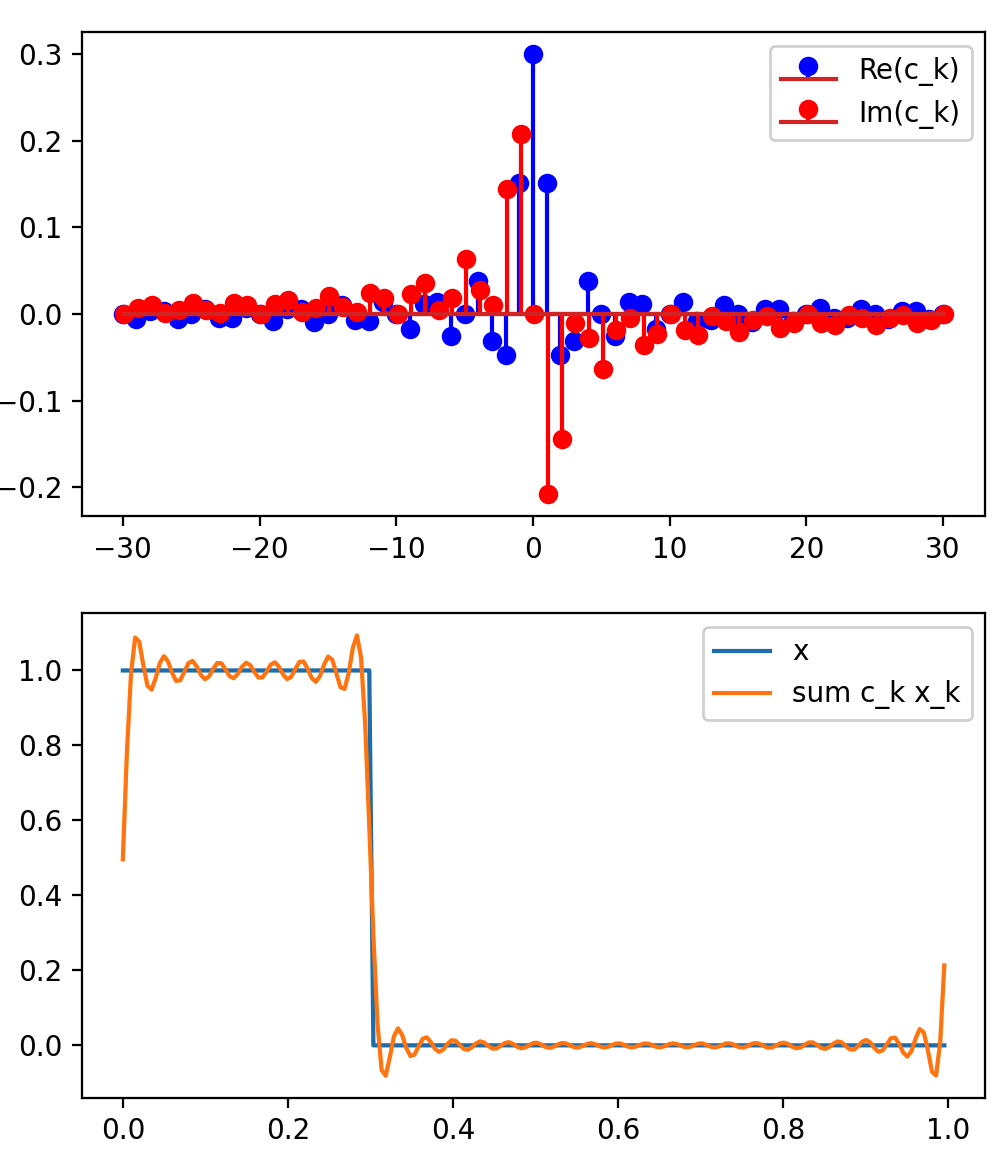
\includegraphics[width=\textwidth]{code/fourier_series.png}
    \end{minipage}
    \codecaption{dsv/code/fourier_series.py}{Berechnung und Darstellung von \eqref{eq:fourier:fourier_series}}\label{py:fourier_series}
\end{listing}

In \Cref{py:fourier_series} wird eine Rechteckfunktion $\Rect_{[0,T]}$ in ihre Fourier-Reihe entwickelt.
In diesem Fall m"ussen wir nat"urlich die Reihenentwicklung abbrechen, da kein $K_{\rm max}$ existiert, sodass $c[k] = 0$ f"ur $k > K_{\rm max}$.
Wir k"onnten die Reihe zwar analytisch ausrechnen, da wir jedes $x_k$ nur auf $[0,T]$ integrieren, also dem Bereich, auf dem die von uns definierte $\Rect_{[0,T]}$-Funktion Werte ungleich $0$ annimmt.
Der Einfachheit halber nutzen wir \texttt{scipy.integrate.quad}, was in der Lage ist numerische Integration relativ pr"azise durchzuf"uhren.

Es lohnt sich mit dem Wert von $K_{\rm max}$ zu experimentieren. 
Man sieht hierbei, dass gr"o"sere Werte von $K_{\rm max}$ an den Unstetigkeitsstellen $0$ und $T$ und in deren N"ahe nicht zu einer besseren "Ubereinstimmung der Fourierreiehe mit $x$ f"uhren.
Die Fourier-Reihe muss also nicht immer gegen $x$ konvergieren.
Im Falle von $\Rect_{[0,T]}$ ergibt sich das Problem genau aus dem Verhalten an $0$ und $T$ -- also Unstetigkeit, was ein generelles Problem bei der Entwicklung von Signalen in Fourier-Reihen darstellt.

Im oberen Plot von \Cref{py:fourier_series} sieht man auch, dass der Realteil der Koeffizienten $\Re{c[\cdot]}$ ein gerades diskretes Signal ist, also $c[k] = c[-k]$.
Der Imagin"arteil $\Im{c[\cdot]}$ hingegen ist ein ungerade Signal, also $c[k] = -c[-k]$\footnote{siehe \Cref{py:even_odd}}. 
Dies liegt daran, dass das Signal lediglich reelle Werte annimmt, weshalb die Symmetrie-Eigenschaften der $c[\cdot]$ allgemein f"ur reelle Signale gelten.

\begin{figure}
    \begin{center}
        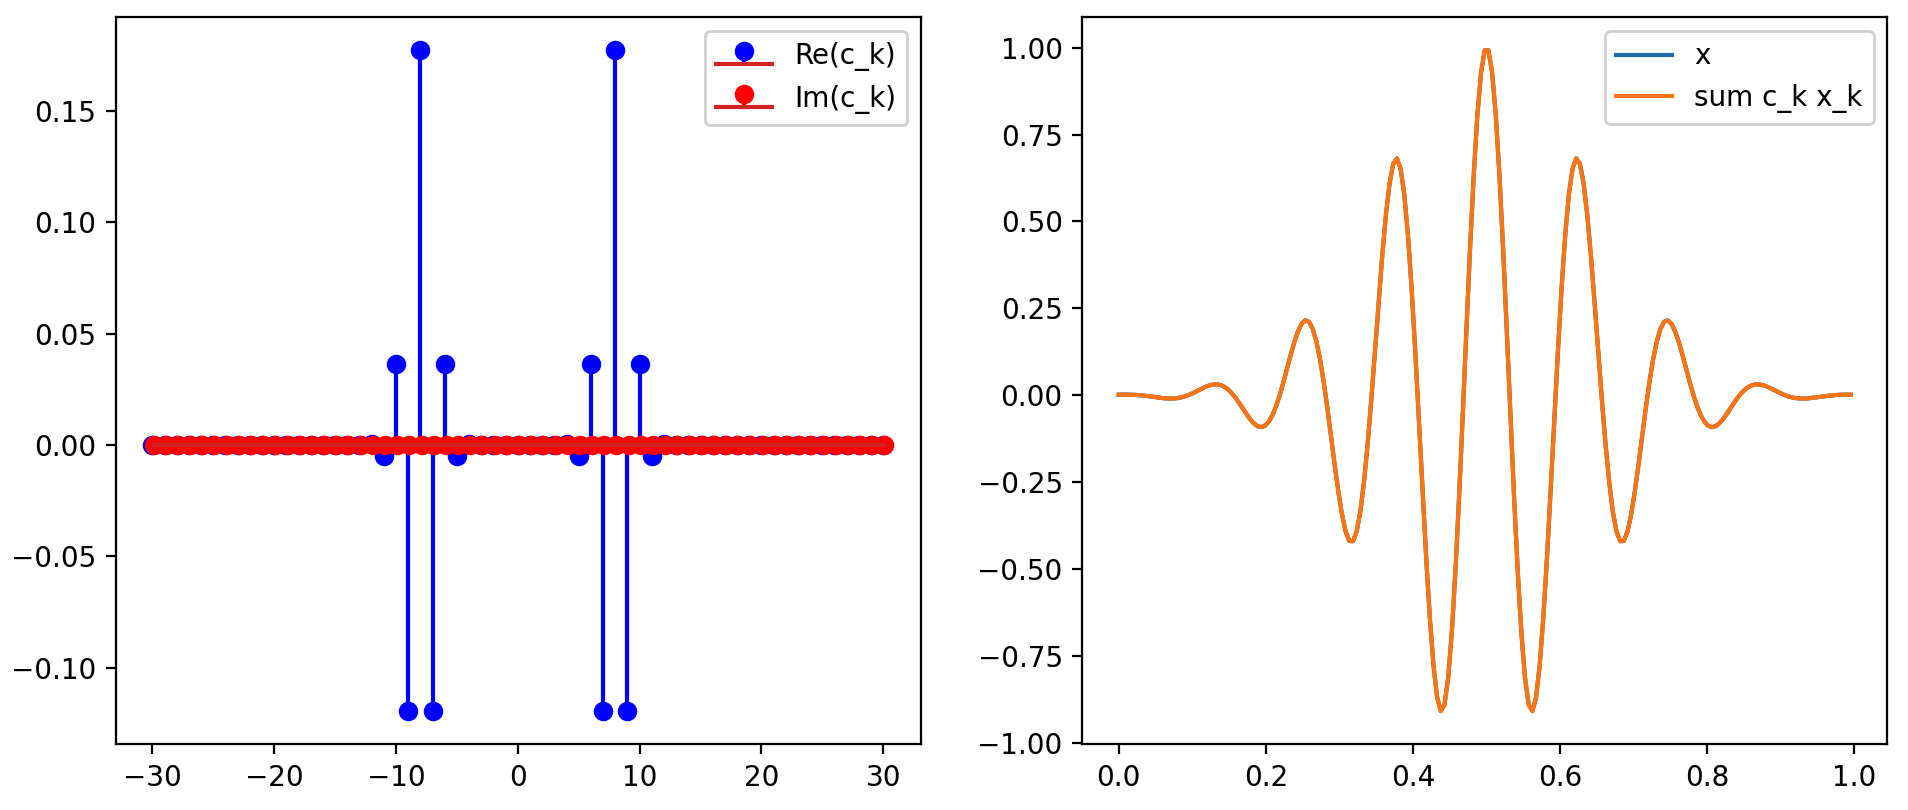
\includegraphics[width=0.8\textwidth]{code/fourier_series_1.png}

        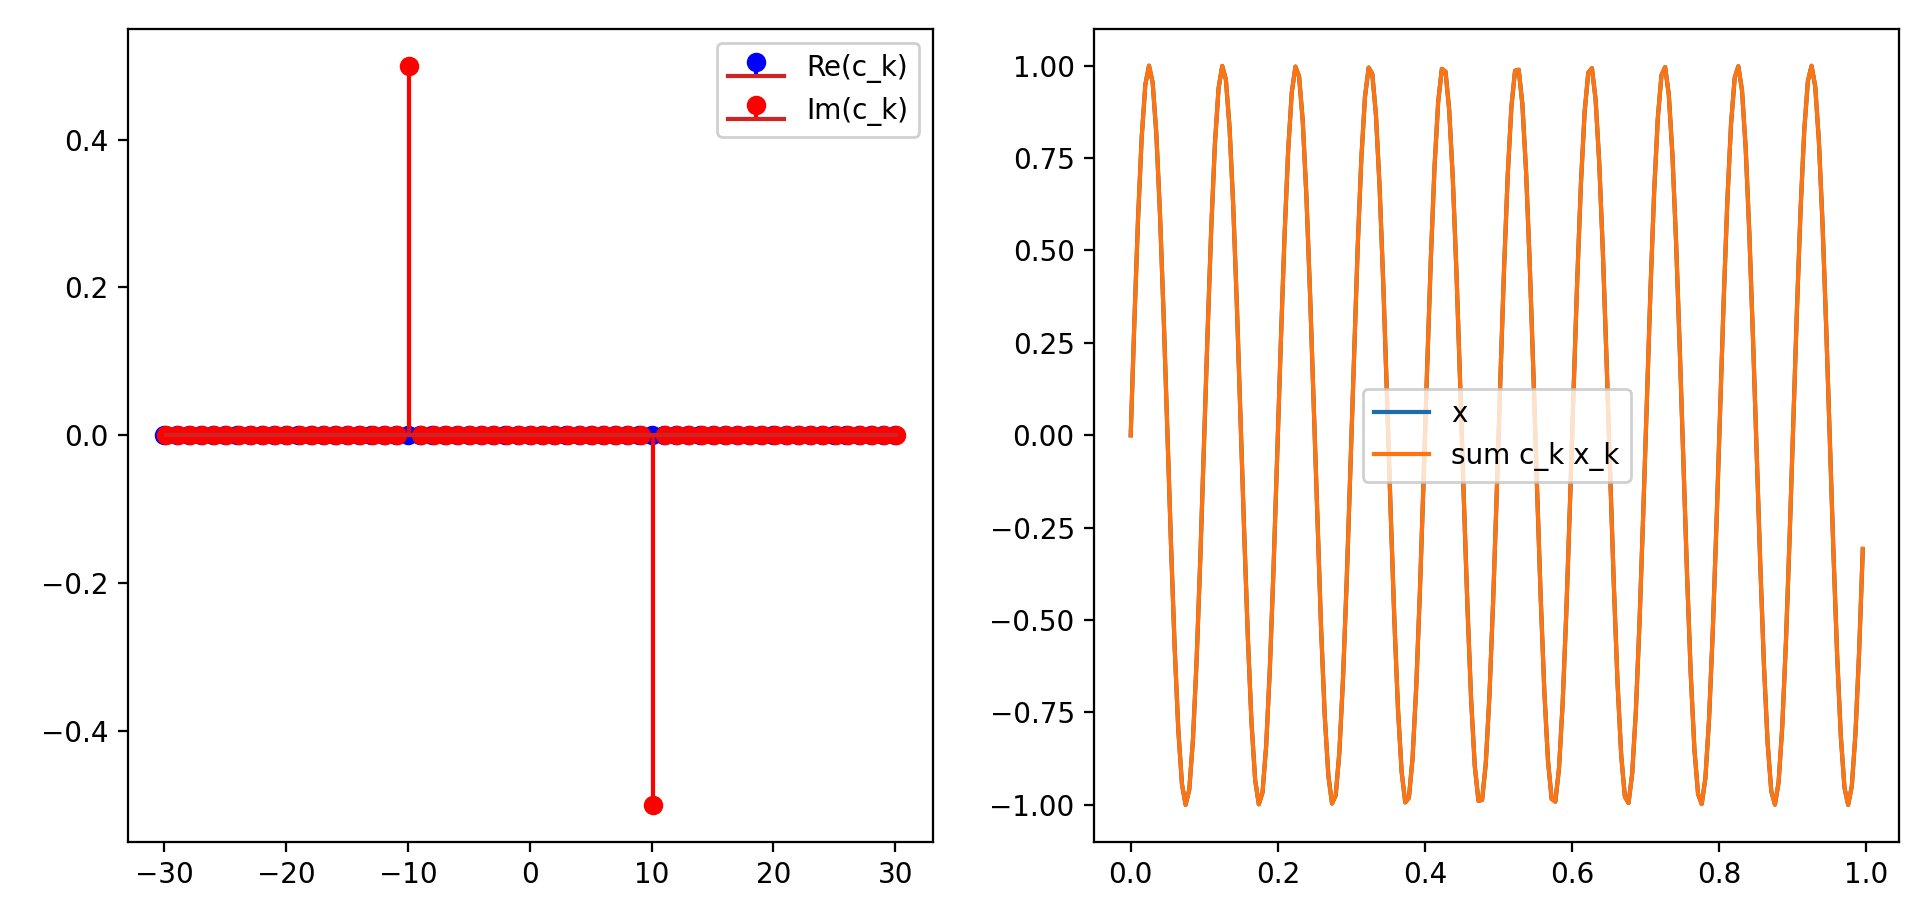
\includegraphics[width=0.8\textwidth]{code/fourier_series_2.png}
    \end{center}
    \caption{Mehr Versionen von \Cref{py:fourier_series}; Oben: $x(t) = \exp(-25(t-0.5)^2) \cos(16 \pi t)$; Unten: $x(t) = \sin(20 \pi t)$;}\label{fig:fourier:fourier_series}
\end{figure}

In \Cref{fig:fourier:fourier_series} sind noch mehr Eigenschaften der Fourier-Reihe deutlich gemacht.
Generell stellen wir fest, dass die beiden Signale jeweils gut durch eine endliche Fourier-Reihe approximiert werden k"onnen, da sie keine Unsteigkeiten aufweisen.
Im oberen Plot sieht man au"serdem, dass Achsen-Symmetrie des Signals $x$ dazu f"uhrt, dass die Imagin"arteile von $c[\cdot]$ verschwinden.
Wie man in \Cref{fig:fourier:fourier_series} unten sieht, ist es bei Anti-Symmetrie des Signals $x$ der Realteil von $c[\cdot]$, der verschwindet.
Dies liegt daran, dass der Realteil der $x_k$ eine gerade Funktion ist und der Imagin"arteil respektive eine ungerade Funktion.
Da wir in \Cref{py:even_odd} schon gesehen haben, dass ungerade und gerade Anteile eines Signals im Sinne von Skalarprodukten orthogonal sind, gilt dies auch f"ur die resultierenden Fourier-Koeffizienten.
In \Cref{fig:fourier:fourier_series} unten sieht man auch, dass man f"ur gewisse Signale die Fourier-Reihe direkt angeben kann.
Im Falle des Beispiels gilt n"amlich
\[
x(t) 
    = \sin(10 \cdot 2 \pi t) 
    = \frac{1}{2 \jmath} \left(
        \exp(10 \cdot 2 \pi t) - \exp(-10 \cdot 2 \pi t)
    \right) 
    = \frac{1}{2 \jmath} x_{10} - \frac{1}{2 \jmath} x_{-10}.
\]
Das hei"st, dass wir $x$ \emph{direkt} in seine Fourier-Reihe entwickelt haben, da wir es als Linearkombination der $x_k$ dargestellt haben.
Das hei"st es sind nur $x_{10}$ und $x_{-10}$ notwendig, um $x$ darzustellen und beide Koeffizienten haben ausschlie"slich imagin"are Anteile.

"Ahnlich wie bei der $z$-Transformation kann man also an der Fourier-Reihe Eigenschaften des Signals $x$ direkt ablesen, oder umgekehrt von Eigenschaften des Signals $x$ auf Eigenschaften der Fourier-Koeffizienten $c[\cdot]$ schlie"sen.
Au"serdem werden wir f"ur die noch folgenden Versionen der \gls{ft} sehr analoge Zusammenh"ange finden.

\subsubsection{Leichtungsdichte-Spektrum periodischer Signale}

Das Leichtungsdichtespektrum eines $T_0$-periodischen Signals $x: \R \rightarrow \C$ is gegeben durch
\begin{equation}\label{eq:fourier:period_psd}
P(x) = \frac{1}{T_0}\Int{0}{T_0}{\Abs{x(t)}^2}{t}
     = \frac{1}{T_0}\Int{0}{T_0}{x(t) x(t)^\ast}{t}
     = \frac{1}{T_0} \ScPr{x}{x}.
\end{equation}
Wir wollen nun $P(x)$ in Abh"angigkeit der Fourier-Koeffizienten $c[\cdot]$ berechnen.
Wir entwickeln also
\[
x(t) = \Sum{k \in \Z}{}{
    c_k \exp(\jmath 2 \pi k F_0 t)
}
\]
und setzen dies in $P$ ein, um
%
\begin{equation}\label{eq:fourier:series_parseval}
    \frac{1}{T_0}\Int{0}{T_0}{x(t) x(t)^\ast}{t}
        = \frac{1}{T_0}\Int{0}{T_0}{
            x(t) 
            \Sum{k \in \Z}{}{
                c_k^\ast \exp(-\jmath 2 \pi k F_0 t)
            }
        }{t}
        = \Sum{k \in \Z}{}{
            c_k^\ast 
            \frac{1}{T_0}\Int{0}{T_0}{
                x(t)
                \exp(-\jmath 2 \pi k F_0 t)
            }{t}
        }
        = \Sum{k \in \Z}{}{
            c_k^\ast c_k
        }
\end{equation}
%
als den \emph{Satz von Parseval}\footnote{\url{https://de.wikipedia.org/wiki/Satz\_von\_Parseval}} zu erhalten.
Die physikalische Interpretation ist, dass $\Abs{c[k]}$ der Leistung des Signals bei der Frequenz $k F_0$ entspricht.
Jeder Index $k$ hat also eine physikalische Gr"o"se, die mit ihm assoziiert ist.

Da nur die Frequenzen $k F_0$ f"ur $k \in \Z$ auftreten, also Frequenzen wie $0.1 F_0$ nicht vorhanden sind, sprechen wir von einem \emph{diskreten Spektrum}.
Es ergibt sich also direkt folgender wichtiger Zusammenhang: Periodische Signale im Zeitbereich besitzen ein \emph{diskretes} Spektrum.
Andersherum ergibt sich auch: Signale mit diskretem Spektrum sind periodisch.
Beide Argument ergeben sich aus der Fourier-Reihe.
Damit haben wir das duale Ergebnis zu \eqref{eq:spectrum_sampled} gefunden.
Dort f"uhrte Diskretisierung im Zeitbereich, also Sampling/Abtastung, zu einer Periodifizierung im Frequenzbereich.

\begin{listing}[ht]
    \noindent
    \begin{minipage}{0.51\textwidth}
        \strut\vspace*{-\baselineskip}\newline
        \inputminted[firstline=5, lastline=14]{python3}{code/period_psd.py}
    \end{minipage}%
    \begin{minipage}{0.48\textwidth}
        \strut\vspace*{-\baselineskip}\newline
        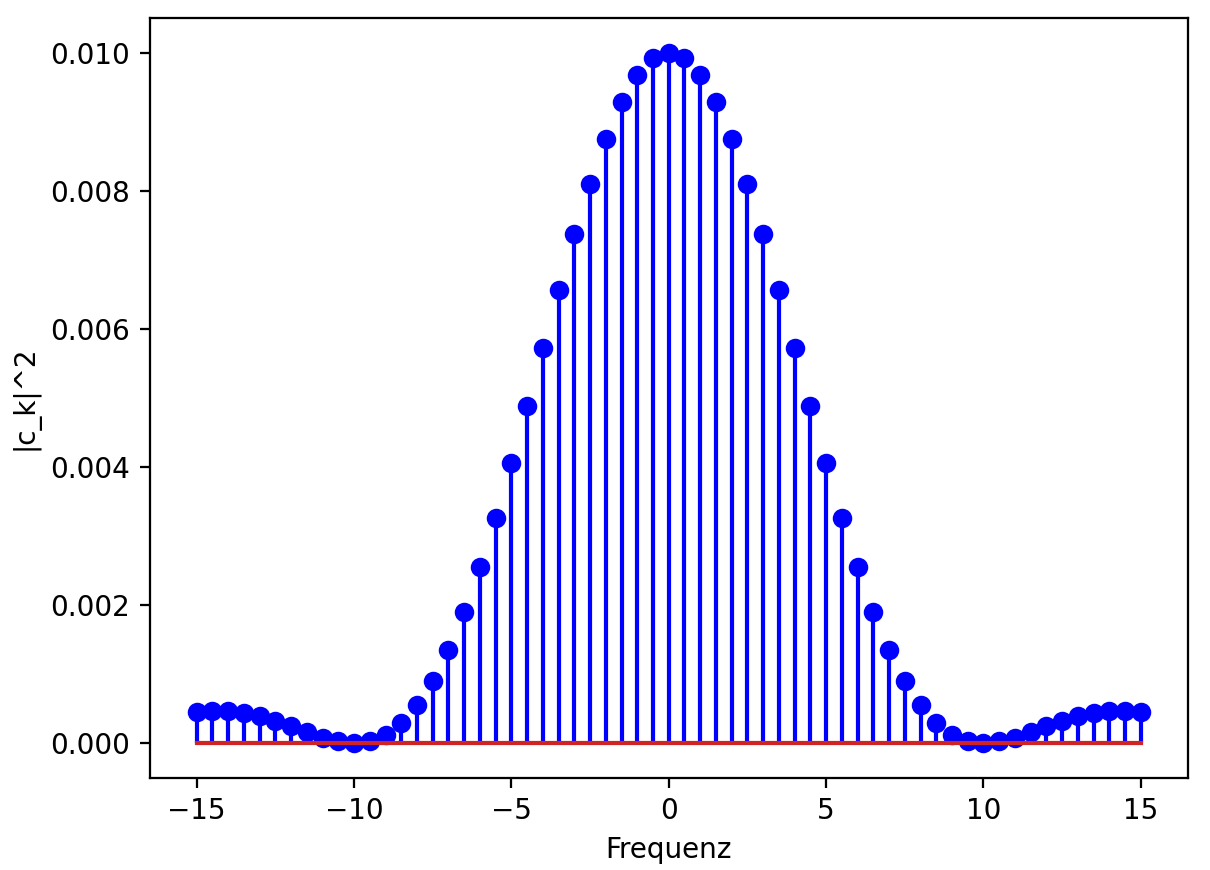
\includegraphics[width=\textwidth]{code/period_psd.png}
    \end{minipage}
    \codecaption{dsv/code/period_psd.py}{Modizifiertes \Cref{py:fourier_series} und Plot von $P$ im Frequenzbereich.}\label{py:period_psd}
\end{listing}

In \Cref{py:period_psd} zeigen wir eine Modifikation von \Cref{py:fourier_series}, in welcher wir $T_0 = 2$ setzen, also $F_0=1/2$ erhalten. 
Auf der Frequenzachse sehen wir, dass demnach diese f"ur $K_{\rm max} = 30$ also von $-15$ bis $+15$ reicht.
%
%
\FloatBarrier
\subsubsection{Fourier-Transformation von kontinuierlichen aperiodischen Signalen}
%
Um die Einschr"ankung auf periodische Signale zu vermeiden, nutzen wir die \acrlong{ft}, wie wir sie bereits in \eqref{eq:sampling:fourier_trafo} f"ur ein Signal $x : \R \rightarrow \C$ durch
\begin{equation}\label{eq:fourier:fourier_trafo}
    X(F) = \Int{-\infty}{+\infty}{x(t) \exp(-\jmath 2 \pi F t)}{t}
\end{equation}
definiert haben.
Im Unterschied zu \eqref{eq:fourier:fourier_series} integrieren wir nun "uber ganz $\R$, da sich das Signal nicht mehr periodisch wiederholt.
Aus diesem Grund ergibt sich auch ein \emph{kontinuierliches} Spektrum, da wir uns nicht mehr auf eine abz"ahlbare Menge von diskreten Frequenzen zur"uckziehen k"onnen.
Deshalb ergibt sich auch f"ur die Synthese des Signals, dass wir auch in diesem Fall integrieren anstatt summieren m"ussen, es gilt also
\begin{equation}\label{eq:fourier:inv_fourier_trafo}
    x(t) = \Int{-\infty}{+\infty}{X(F) \exp(\jmath 2 \pi F t)}{F}.
\end{equation}
Da sich f"ur die meisten Signale, die wir betrachten werden, Integration und Summation \q{"ahnlich} verhalten, finden wir auch die obigen Eigenschaften bez"uglich Symmetrien, etc., von \eqref{eq:fourier:fourier_series} wieder.

Es gibt aber eine Verbindung zur Fourier-Reihe, die wir im Folgenden kurz erl"autern wollen.
Nehmen wir an, es existiert ein $T > 0$, sodass $\Abs{x(t)} = 0$ f"ur alle $t$ mit $\Abs{t} > T$.
Dann k"onnen wir das Signal $x$ periodifizieren mit Periode $T$, indem wir
\[
x_p(t) = \Sum{k \in Z}{}{x(t - 2kT)}
\]
setzen.
Dies haben wir bereits in "ahnlicher Form in \eqref{eq:spectrum_sampled} gesehen. 
Dort hat es sich aber aus Berechnungen ergeben und hier \emph{setzen} wir diesen Zusammenhang explizit.
Dann k"onnen wir $x_p$ in seine Fourier-Reihe 
\[
x_p(t) = \Sum{k \in \Z}{}{c_k \exp(\jmath 2 \pi k t/T)}
\Text{mit}
T\,c_k = \Int{-T/2}{+T/2}{x_p(t) \exp(- \jmath 2 \pi k t/T)}{t}
    = \Int{-\infty}{+\infty}{x(t) \exp(- \jmath 2 \pi k t/T)}{t}
\]
entwickeln.
Aus der Definition in \eqref{eq:fourier:fourier_trafo} und der letzten Gleichung sehen wir, dass sich die Koeffizienten der Fourier-Reihe finden lassen durch
\begin{equation}\label{eq:fourier:c_k_fourier}
    c_k = \frac 1T X\left(\frac kT\right),
\end{equation}
diese sich also auch aus der Fourier-Transformation ablesen lassen.
Das hei"st, dass wir auch
\[
x_p(t) = \Sum{k \in \Z}{}{\frac 1T X\left(\frac kT\right) \exp(\jmath 2 \pi k t/T)}
       = \Sum{k \in \Z}{}{X\left(k \Delta F\right) \exp(\jmath 2 \pi k t \Delta F) \Delta F}
\]
schreiben k"onnen.
Dabei haben wir im letzten Schritt $1/T = \Delta F$ gesetzt.
Dies k"onnen wir intuitiv (aber nicht rigoros!) so interpretieren, dass im Falle von $T \rightarrow \infty$ gilt, dass $\Delta F \rightarrow 0$.
Je l"anger der Bereich der Funktion $x$, auf welchem gilt $x \neq 0$, desto kleiner $\Delta F$.
Der nicht-periodische Fall $T = \infty$ ergibt sich also als Grenzfall, bei welchem obige Summation zu einer Integration wird und $\Delta F$ zu einem $\mathrm{d}F$.
Man kann die \acrlong{ft} also als Grenzfall der Fourier-Reihe f"ur $T \rightarrow \infty$ betrachten.
%
%
\subsubsection{Leistungsdichte-Spektrum aperiodischer Signale}
%
Analog zum Satz von Parseval f"ur periodische Signale in \eqref{eq:fourier:series_parseval} k"onnen wir auch hier wieder definieren und folgern, dass
\begin{equation}
E(x) = \Int{-\infty}{+\infty}{\Abs{x(t)}^2}{t}
     = \Int{-\infty}{+\infty}{\Abs{X(F)}^2}{F}
\end{equation}
auch wieder ein Parseval Theorem f"ur die \acrlong{ft} ergibt, was aber in diesem Fall als Plancherel Theorem\footnote{\url{https://en.wikipedia.org/wiki/Plancherel_theorem}} genannt wird.

Andererseits kann man $X$ auch in Betrag und Phase zerlegen, da es im Allgemeinen eine komplexe Gr"o"se ist, also
\[
X(F) = \Abs{X(F)} \exp(\jmath \angle(X(F))).
\]
Man nennt dann $\Abs{X(F)}^2$ das \emph{Leistungsdichte-Spektrum} von $x$.

\begin{listing}[ht]
    \noindent
    \begin{minipage}{0.51\textwidth}
        \strut\vspace*{-\baselineskip}\newline
        \inputminted[firstline=6, lastline=45]{python3}{code/fourier_trafo.py}
    \end{minipage}%
    \begin{minipage}{0.48\textwidth}
        \strut\vspace*{-\baselineskip}\newline
        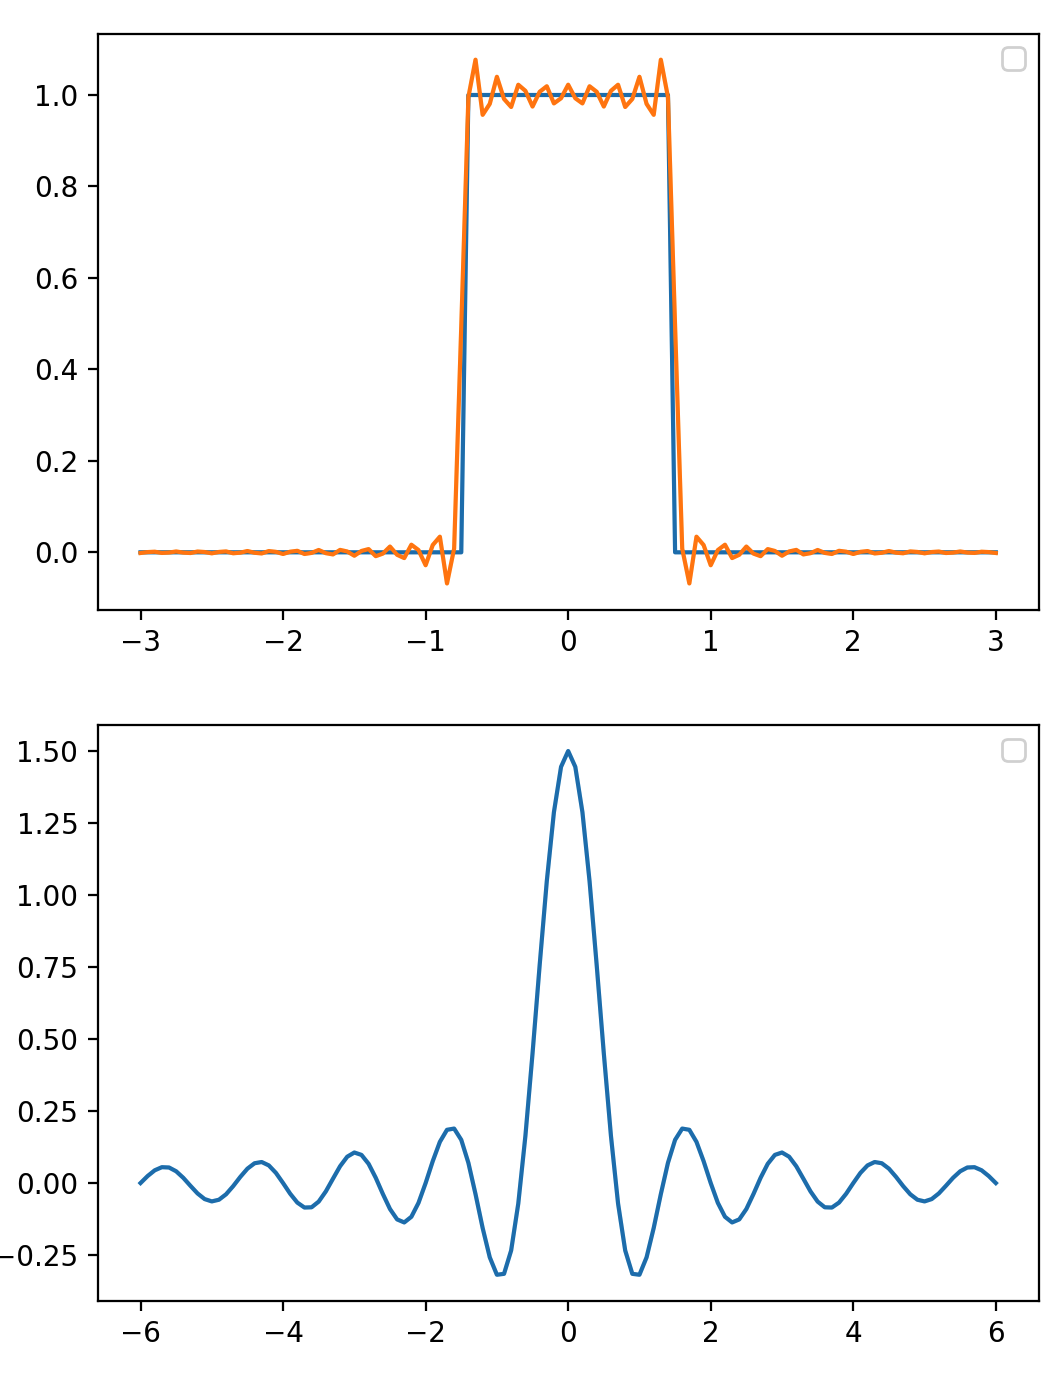
\includegraphics[width=\textwidth]{code/fourier_trafo.png}
    \end{minipage}
    \codecaption{dsv/code/fourier_trafo.py}{Berechnung und Darstellung von \eqref{eq:fourier:fourier_trafo}}\label{py:fourier_trafo}
\end{listing}

In \Cref{py:fourier_trafo} zeigen wir das Vorgehen zur Fourier-Analyse mittels numerischer Integration.
Es ist hier anzumerken, dass wir \q{nur} die Funktion \texttt{rect} definieren m"ussen und der Rest, also die Funktionen \texttt{kernel}, \texttt{analyse} und \texttt{synthese} unabh"angig hiervon sind.
Wir haben hier ein \namecref{py:fourier_trafo}, welches sich Methoden der Funktionalen Programmierung bedient.
Die Funktionen texttt{analyse} und \texttt{synthese} haben als Eingabewert die entweder die Funktion, oder die \acrlong{ft} einer Funktion.
Au"serdem liefern sie als Ausgabewert wieder \emph{Funktionen}, die wir einfach \q{aufrufen} k"onnen.
%
\subsection{Fourier-Transformation diskreter Signale}\label{sec:fourier:disc}
%
Wir n"ahern uns langsam der Fourier-Analyse von diskreten Signalen.
Schlie"slich wollen wir etwaige spektrale Analysen und dergleichen im Digitalen durchf"uhren, um die Vorz"uge von digitalen Rechenwerken dabei nutzen zu k"onnen.
Die vorher eingef"uhrten Transformationen sind zwar hilfreich f"ur theoretische Argumentation, wie beispielsweise beim Sampling-\Cref{stm:sampling_theorem}. 
Deshalb wenden wir uns nun der spektralen Analyse von diskreten Signalen zu.
Wir werden aber im Verlauf auch wieder "ahnliche Zusammenh"ange wie in \eqref{eq:fourier:c_k_fourier} finden.
%
\subsubsection{Fourier-Transformation diskreter periodischer Signale}\label{sec:fourier:disc_period}
%
Wir beginnen mit diskreten Signalen, die gleichzeitig periodisch sind, also ein $N$ existiert, sodass
\[
x[n] = x[n+kN] \Text{f"ur alle} n,k \in \Z 
\]
gilt.
Aus vorherigen Diskussionen in \Cref{sec:sampling} wissen wir einerseits, dass diskrete Signale ein periodisches Spektrum auf $(0,1)$ besitzen.
Andererseits wissen wir aus \Cref{sec:fourier:cont:period}, dass periodische Signale ein \emph{diskretes} Spektrum besitzen.
Wir finden also nun intuitiv, dass das Spektrum von diskreten periodischen Signalen \emph{ebenfalls} diskret und periodisch ist.
Denken wir zur"uck an \Cref{sec:sampling:disc_sin} so haben wir bereits alles Notwendige betrachtet.
Ein $N$-periodisches diskretes Signal ergibt sich aus der Linearkombination der diskreten Signale $x_k[\cdot] : \Z \rightarrow \C$ definiert durch
\[
x_k[n] = \exp\left(\jmath 2 \pi \frac k N n \right) \Text{mit} k = 0, \ldots, N-1.
\]
Das hei"st, f"ur $x[\cdot]$ setzen wir mit
\[
x[\cdot] = \Sum{k = 0}{N-1}{c[k] x_k[\cdot]}
\]
an.
Damit sind bereits beide Eigenschaften des Spektrums \q{eingepreist}.
Denn man erkennt in den $x_{k}[\cdot]$ die vorher erw"ahnte \emph{zweifache} Periodizit"at wieder, weil sowohl $x_{k+N}[\cdot] = x_{k}[\cdot]$ f"ur alle $k$ als auch $x_k[n+N] = x_k[n]$ f"ur alle $n$ gilt.

Es ist nun unser Ziel f"ur gegebene Werte $x[n]$ von $x[\cdot]$ die Werte des \emph{ebenfalls periodischen und diskreten} Signals $c[\cdot]$ zu bestimmen.
Dies verl"auft ganz analog zu \Cref{sec:fourier:cont:period}.
Wir definieren das Skalarprodukt $\ScPr{\cdot}{\cdot}$ f"ur $N$-periodische und diskrete Signale via
\[
\ScPr{x_1[\cdot]}{x_2[\cdot]} 
    = \Sum{n = 0}{N-1}{x_1[n] x_2[n]^\ast}.
\]
Das hei"st, dass wir periodisches Signal $x[\cdot]$ mit dem \emph{endlich-dimensionalen} Vektor $\bm x \in \C^{N}$ identifizieren, wir setzen also die Eintr"age des Vektors als $\bm x_i = x[i-1]$.
Dann k"onnen wir auch f"ur das entsprechende Skalarprodukt der Vektoren $\bm x_{1,2} \in \C^N$
\[
\ScPr{\bm x_1}{\bm x_2} 
    = \left(\bm x_2^\ast\right)^\trans \cdot \bm x_1 
    = \bm x_2^\herm \cdot \bm x_1
\]
schreiben.
Analog identifizieren wir die periodische und diskrete Sequenz $c[\cdot]$ mit dem Vektor $\bm c \in \C^N$.

Wie in \Cref{sec:fourier:cont:period} m"ussen wir nur 
\[
\ScPr{\bm x_k}{\bm x_\ell} 
    = \Sum{i=0}{N-1}{
        x_k[i] x_\ell[i]^\ast
    }
    = \Sum{i=0}{N-1}{
        \exp\left(\jmath 2 \pi \frac{i(k-l)}{N} \right)
    }
    = \begin{cases}
        N \Text{falls} k = \ell \\
        \frac{
            1 - \exp\left(\jmath 2 \pi \frac{(k-l)}{N} \right)^N   
        }{
            1 - \exp\left(\jmath 2 \pi \frac{(k-l)}{N} \right)
        } \Text{sonst}
    \end{cases}
    = \begin{cases}
        N \Text{falls} k = \ell \\
        0 \Text{sonst}
    \end{cases}
\]
berechnen.
Hierbei nutzen wir, dass $\exp(\jmath 2 \pi k) = 1$ f"ur alle $k \in \Z$.
Wie in \Cref{sec:fourier:cont:period} finden wir, dass also gilt $\ScPr{\bm x_k}{\bm x_\ell} = 0$, falls $k \neq \ell$ und $\ScPr{\bm x_k}{\bm x_k} = N$.
Damit ergibt sich bei Anwendung auf das eigentliche Signal $\bm x$ f"ur den Vektor $\bm c$, dass
\[
\ScPr{\bm x}{\bm x_\ell}
    = \ScPr{\Sum{k=1}{N}{\bm c_k \bm x_k}}{\bm x_\ell}
    = \Sum{k=1}{N}{\bm c_k \ScPr{\bm x_k}{\bm x_\ell}}
    = N \bm c_\ell
\Rightarrow
\bm c_\ell = \frac{1}{N}\ScPr{\bm x}{\bm x_\ell}.
\]
Zusammenfassend, kann man also sagen, dass sich folgende Analyse- und Synthesegleichungen ergeben:
\begin{equation}\label{eq:fourier:disc_analys_synth}
    x[n] = \Sum{k = 0}{N-1}{c[k]\exp(\jmath 2 \pi k n/N)}, \Text{und}
    c[k] = \frac{1}{N}\Sum{n = 0}{N-1}{x[n]\exp(-\jmath 2 \pi k n/N)}.
\end{equation}
In Vektorschreibweise l"asst sich der erste Teil durch
\begin{equation}\label{eq:fourier:disc_analys_synth_vec}
    \bm x = \Sum{k = 0}{N-1}{\ScPr{\bm x}{\bm x_k} \bm x_k}
\end{equation}
ausdr"ucken.

Weiterhin, k"onnen wir eine Matrix $\bm F_N \in \C^{N \times N}$ definieren, deren $k$-te Spalte den Vektor $\bm x_k$ beinhaltet.
Wir definieren also 
\[
\bm F_N = \left[
    \bm x_1, \ldots, \bm x_k, \ldots, \bm x_N 
\right]
\]
Dann k"onnen wir noch einen Schritt weitergehen und sehen, dass
\[
\bm c = \frac{1}{N} \bm F_N^\herm \bm x, \Text{und} \bm x = \bm F_N \bm c
\]
gilt.
Das hei"st, dass sich Fourier-Analyse und Fourier-Synthere von diskreten und periodischen Signalen durch eine Matrix-Vektor-Multiplikation durchf"uhren l"asst!
Das sind erst einmal gute Nachrichten, denn damit wissen wir, dass digitale Rechenwerke sehr gut darin sind, diese Transformation durchzuf"uhren.
Die hier vorgestellte Transformation nennen wir \gls{dft} und oft definiert man ein diskretes Signal $X[\cdot]$ durch
\begin{equation}
    X[k] = \frac{1}{N}\Sum{n = 0}{N-1}{x[n]\exp(-\jmath 2 \pi k n/N)} = c[k] = \bm c_k
\end{equation}
und nennt dieses dann die \gls{dft} von $x[\cdot]$.
Es ist anzumerken, dass der Vorfaktor $N^{-1}$ in manchen Lehrb"uchern oder Ver"offentlichungen auch bei der Synthese anstatt der Analyse auftaucht, oder aber \emph{beide} Gleichungen erhalten einen Faktor $N^{-1/2}$.

In \Cref{py:dft_1} zeigen wir ein einfaches Beispiel f"ur $x[\cdot] = u[\cdot] - u[\cdot-k]$.
Au"serdem zeigen wir auch die beiden Berechungsmethoden der $c[\cdot]$ -- einerseits mit der Definition und andererseits "uber ein Matrix-Vektor-Produkt.
%
\begin{listing}[ht]
    \noindent
    \begin{minipage}{0.51\textwidth}
        \strut\vspace*{-\baselineskip}\newline
        \inputminted[firstline=5, lastline=23]{python3}{code/dft_1.py}
    \end{minipage}%
    \begin{minipage}{0.48\textwidth}
        \strut\vspace*{-\baselineskip}\newline
        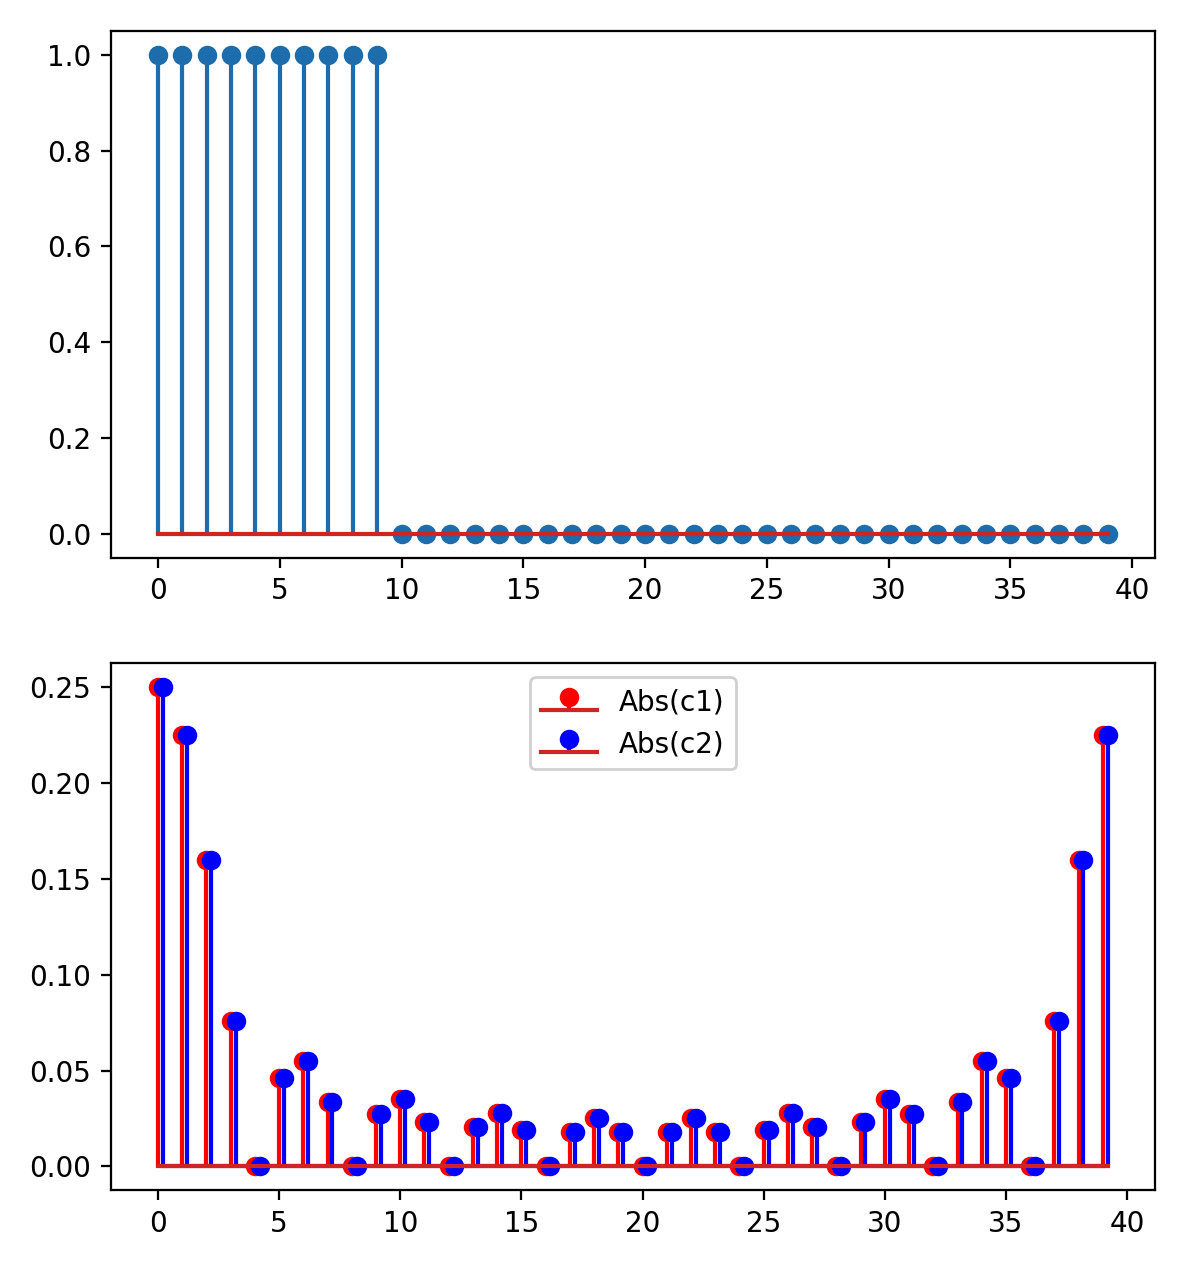
\includegraphics[width=\textwidth]{code/dft_1.png}
    \end{minipage}
    \codecaption{dsv/code/dft_1.py}{Berechnung und Darstellung von \eqref{eq:fourier:disc_analys_synth}}\label{py:dft_1}
\end{listing}
%
\subsubsection{Leichtungsdichte-Spektrum diskreter periodischer Signale}\label{sec:fourier:disc_period_power}
%
Da periodische Signale keine endliche Energie besitzen, betrachten wir die durchschnittliche Leistung "uber eine Periode.
Wir betrachten also f"ur ein $N$-periodisches Signal $x[\cdot]$ das Funktional
\begin{equation}
    P(x[\cdot]) = \frac{1}{N}\Sum{i=0}{N-1}{\Abs{x[n]}^2}.
\end{equation}
Dann k"onnen wir ganz analog zu vorher wieder herleiten, dass f"ur
\[
x[\cdot] = \Sum{i=0}{N-1}{c[k] x_k[\cdot]}
\]
und dessen Leistung gilt, dass
\[
P(x[\cdot]) = \Sum{i=0}{N-1}{\Abs{c[k]}^2}.
\]
Also auch hier finden wir wieder, dass sich die durchschnittliche Leistung einer Periode im Zeitbereich auf die Leistung einer Periode im Frequenzbereich "ubertr"agt.
Auch hier k"onnen wir die Folge $\Abs{c[\cdot]}^2$ als Leistungsdichte-Spektrum interpretieren.
\FloatBarrier
%
\subsubsection{Fourier-Transformation diskreter aperiodischer Signale}\label{sec:fourier:disc_aperiod}
%
Wiederum analog zu \Cref{sec:fourier:cont} ben"otigen wir noch eine Transformation f"ur diskrete Signale, die keine Periodizit"at aufweisen.
Hierzu definieren wir die zugeh"orige Fourier-Transformation, die wir \gls{dtft} nennen, durch
\begin{equation}\label{eq:fourier:dtft}
    X(f) = \Sum{n \in \Z}{}{x[n] \exp(-\jmath 2 \pi f n)},
\end{equation}
genau wie in \Cref{sec:sampling} bei der Herleitung von \eqref{stm:sampling_theorem}.
Im Unterschied zur \q{analogen} Fourier-Transformation \eqref{eq:fourier:fourier_trafo} sehen wir, dass $X$ nur f"ur Frequenzen $f \in (0,1]$ definiert ist, da das diskrete Signal $x_f[n] = \exp(\jmath 2 \pi f n)$ periodisch in $f$ ist.
Es gilt also $x_{f + k}[\cdot] = x_{f}[\cdot]$ f"ur alle $k \in \Z$.
Dies \q{passt} auch zur Natur von diskreten Signalen, da deren Frequenzbereich \emph{immer} periodisch sein muss.

Wir k"onnen nun f"ur die inverse Transformation \eqref{eq:fourier:dtft} mit \eqref{eq:fourier:fourier_series} vergleichen. 
Bis auf das Vorzeichen in der Funktion $\exp()$ gleicht \eqref{eq:fourier:dtft} einer Fourier-Reihe der periodischen Funktion $X$.
In der Tat, k"onnen wir die Folge $x[\cdot]$, also das urspr"ungliche Signal, als Fourier-Koeffizienten der \gls{dtft} $X$ durch
\begin{equation}\label{eq:fourier:idtft}
    x[n] = \Int{-1/2}{+1/2}{X(f)\exp(\jmath 2 \pi f n)}{f}
\end{equation}
wiederfinden.
Diese Synthese-Operation nennen wir dann \gls{idtft}.
Es ist wiederum anzumerken, dass die \gls{dtft} \q{nur} ein theoretisches Werkzeug ist, da sich im Allgemeinen die unendliche Summe in \eqref{eq:fourier:dtft} praktisch nicht realisieren l"asst, genauso wenig wie deren Resultat, eine kontinuierliche Funktion.

In \Cref{py:dtft} zeigen wir dennoch, wie man die \gls{dtft} einer aperiodischen Folge approximieren kann.
Wir studieren hierzu das Signal
\[
x[n] = \begin{cases}
    \frac{\omega}{\pi} \Text{f"ur} n = 0,\\
    \frac{\omega}{\pi} \frac{\sin(\omega n)}{\omega n} \Text{sonst}.
\end{cases}
\]
Dessen analytisch bestimmte \gls{dtft} $X$ ist
\[
X(f) = \Rect(f/(2 \pi \omega)),
\]
welche wir durch eine endliche Summe "uber die von uns verf"ugbaren Werte von $x[\cdot]$ bestimmen.

Nun treten hierbei mehrere Effekte zutage.
%
\begin{itemize}
\item Die Approximation der \gls{dtft} mittels des \q{abgeschnittenen} Signals $x$ stimmt noch nicht sehr gut mit der analytischen L"osung "uberein. 
Ver"andert man den Wert der Variable $N$ im Skript, tritt dieser Effekt st"arker oder schw"acher zutage.
\item Auch bei Erh"ohung von $N$ stellt sich immernoch keine Konvergenz von $X_{\rm approx}$ gegen $X_{\rm true}$ ein.
Dies liegt daran, dass die \gls{dtft} von $x[\cdot]$ nicht konvergiert, wie wir in \Cref{py:fourier_series} bereits gesehen hatten.
Diesen Effekt bezeichnet man allgemein als Gibbssches Ph"anomen\footnote{\url{https://en.wikipedia.org/wiki/Gibbs_phenomenon}}.
\item Augenscheinlich ist es besser die \gls{idtft} aus $X_{\rm approx}$ zu berechnen, als aus $X_{\rm true}$. Doch dies liegt legidlich daran, dass die numerische Integration der $\Rect$-Funktion nicht genau genug ist.
Erh"oht man die Anzahl der Punkte im Array \texttt{F}, dann stimmen im dritten Plot die drei Graphen besser "uberein.
\end{itemize}
%
\begin{listing}[ht]
    \noindent
    \begin{minipage}{0.51\textwidth}
        \strut\vspace*{-\baselineskip}\newline
        \inputminted[firstline=5, lastline=48]{python3}{code/dtft.py}
    \end{minipage}%
    \begin{minipage}{0.48\textwidth}
        \strut\vspace*{-\baselineskip}\newline
        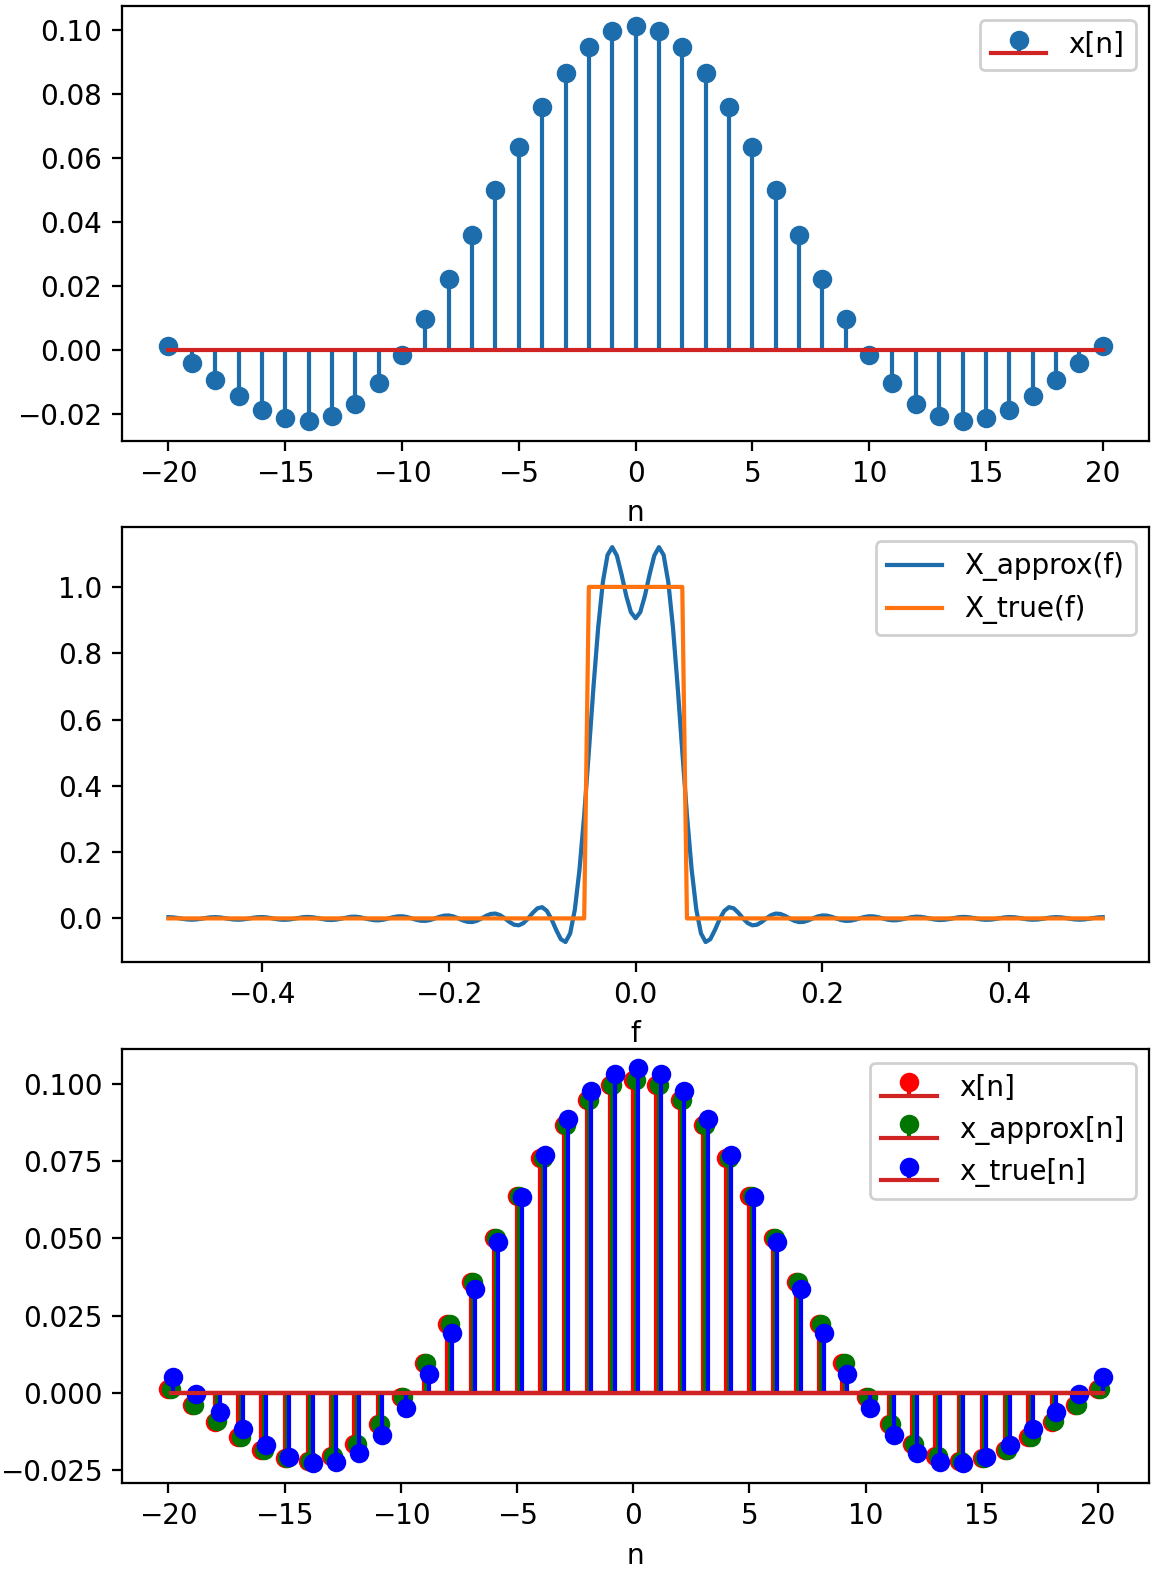
\includegraphics[width=\textwidth]{code/dtft.png}
    \end{minipage}
    \codecaption{dsv/code/dtft.py}{Berechnung und Darstellung von \eqref{eq:fourier:dtft}}\label{py:dtft}
\end{listing}
%
\FloatBarrier
\subsubsection{Leichtungsdichte-Spektrum diskreter aperiodischer Signale}\label{sec:fourier:disc_aperiod_power}
%
Die Energie eines diskreten Signals haben wir in \eqref{eq:disc_sig_energy} durch
\[
\mathcal{E}(x[\cdot]) = \Sum{n \in \Z}{}{\Abs{x[n]}^2} 
\]
definiert.
Wiederum k"onnen wir uns "uberlegen, dass dann f"ur die \gls{dtft} $X$ gilt, dass
\[
\mathcal{E}(x[\cdot]) = \Int{-1/2}{+1/2}{\Abs{X(f)}^2}{f}.
\]
Schlussendlich bezeichnet man dann
\[
S_{xx}(f) = \Abs{X(f)}^2
\]
als das Leichtungsdichte-Spektrum des Signals $x[\cdot]$.
In manchen Anwendungen ist es auch wieder sinnvoll Betrag und Phase von $X(f)$ zu analysieren.
%
\subsection{Eigenschaften der Fourier-Transformationen}\label{sec:fourier:proper}
%
Nachdem wir nun die notwendigen Definitionen gesammelt haben, wollen wir uns einige wichtige Eigenschaften der definierten Transformationen ansehen und eventuell auch f"ur \q{praktische} Dinge verwenden.
%
\subsubsection{Beziehung der Fourier-Transformationen und der \texorpdfstring{$z$}{z}-Transformation}
%
Wie wir in \cref{sec:ztrafo} gesehen haben, ist die $z$-Transformation f"ur ein diskretes Signal $x[\cdot]$ definiert durch
\[
X_{\z}(z) = \Sum{n \in \Z}{}{x[n]z^{-n}} \Text{mit \gls{roc}} r_2 < \Abs{z} < r_1.
\]
Wenn wir nun $z$ in Polarform $z = r \exp(\jmath 2 \pi f)$ ausdr"ucken und annehmen, dass $r_2 < r , r_1$, dann sehen wir, dass die $z$-Transformation von $x[\cdot]$ nichts anderes ist als die \gls{dtft} von $x[n] r^{-n}$ ist.
Mit anderen Worten ist die $z$-Transformation an einer Stelle $z=r \exp(\jmath 2 \pi f)$ die \gls{dtft} $X$ eines Signals gewichtet mit der Folge $w[n] = r^{-n}$ an der Stelle $f$.
Ist nun $1 \in \gls{roc}$ (und damit der gesamte Einheitskreis der komplexen Ebene), dann gilt
\begin{equation}\label{eq:fourier:ztrafo}
    X_{\z}(\exp(\jmath 2 \pi f)) = X(f)
\end{equation}
Wir haben uns zwar bis jetzt wenig Gedanken "uber die Existenz der Fourier-Transformation gemacht, doch hier finden wir einen Hinweis. 
Die \gls{dtft} existiert, beziehungsweise \emph{konvergiert}, falls $1 \in \gls{roc}$.
Da die \q{Form} der \gls{roc} immer kreisf"ormig ist, ist die gleichbedeutend mit der Tatsache, dass sich der Einheitskreis der komplexen Ebene in der \gls{roc} befindet.
Au"serdem kann man auch eine Fourier-Analyse von \gls{lti}-Systemen betreiben. 
Dann ist die \gls{bibo}-Stabilit"at von einem solchen System "aquivalent zur Tatsache, dass der Einheitskreis in der \gls{roc} liegt.
Wie wir gerade gesehen haben, folgt dann auch, dass \gls{bibo}-Stabilit"at ebenfalls durch die \emph{Existenz} der \gls{dtft} charakterisiert wird.
%
\begin{listing}[ht]
    \noindent
    \begin{minipage}{0.51\textwidth}
        \strut\vspace*{-\baselineskip}\newline
        \inputminted[firstline=5, lastline=46]{python3}{code/dtft_z.py}
    \end{minipage}%
    \begin{minipage}{0.48\textwidth}
        \strut\vspace*{-\baselineskip}\newline
        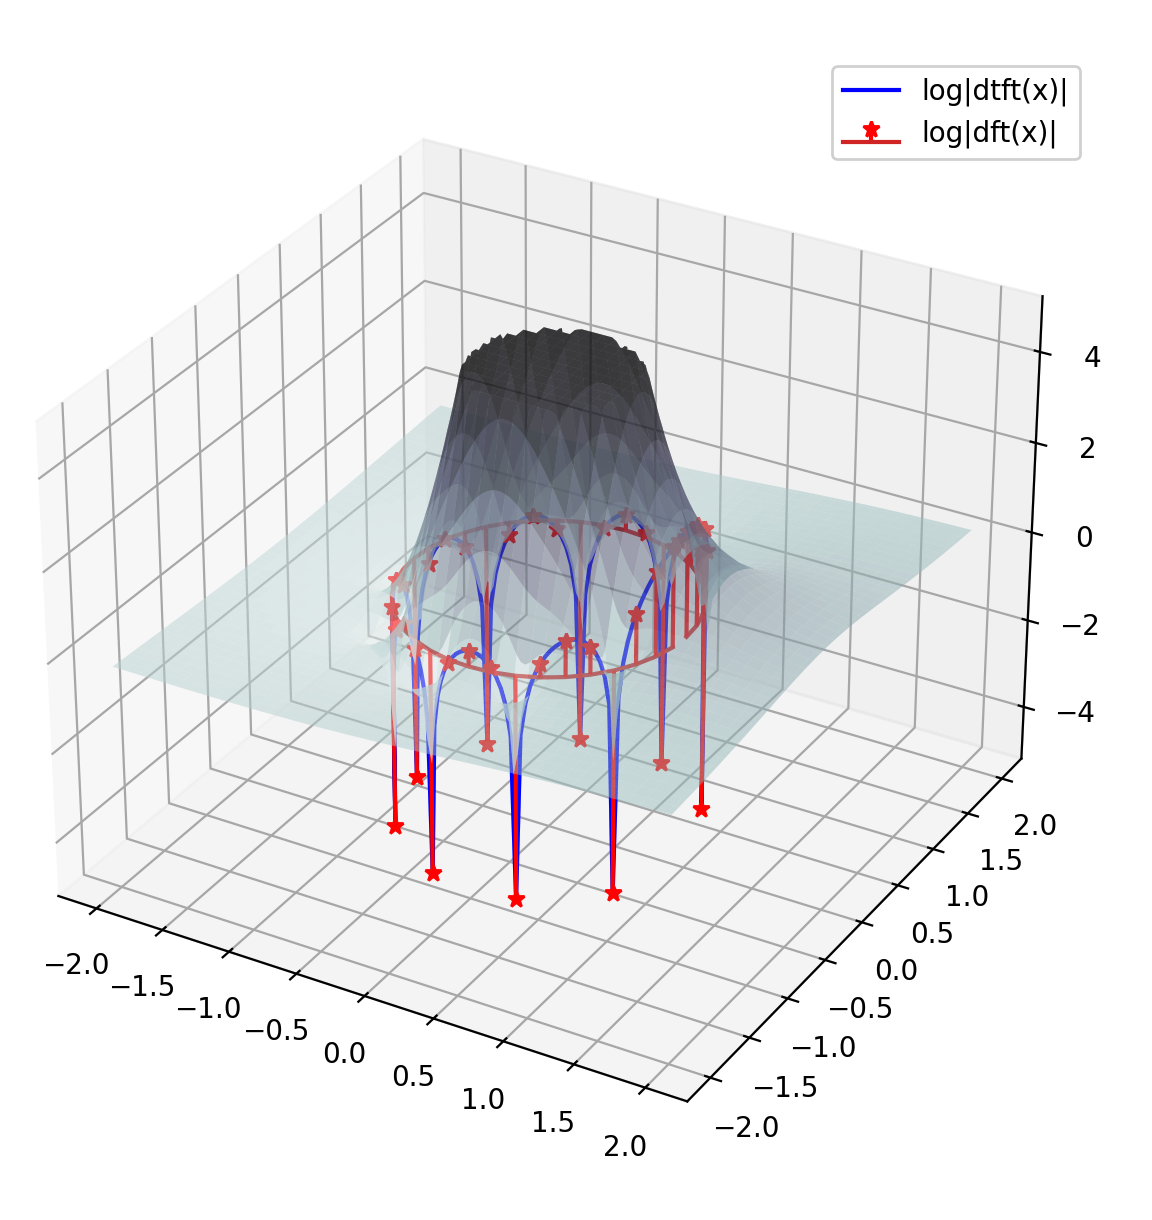
\includegraphics[width=\textwidth]{code/dtft_z.png}
    \end{minipage}
    \codecaption{dsv/code/dtft_z.py}{Berechnung und Darstellung von \eqref{eq:fourier:ztrafo}}\label{py:dtft_z}
\end{listing}

In \Cref{py:dtft_z} zeigen wir diesen Zusammenhang f"ur das gleiche Signal, wie in \Cref{py:dft_1}, interpretieren es hier aber einmal als aperiodisches Signal bei der Berechnung der \gls{dtft} und als periodisches Signal f"ur die Berechung der \gls{dft}.
Wir wissen aus den Eigenschaften der $z$-Transformation, dass das Signal $x[n] = u[n] - u[n-k]$ im $z$-Bereich einen $k$-fachen Pol bei $z = 0$ hat und $k-1$ Nullstellen auf dem Einheitskreis.

Wir k"onnen in dem Plot von \Cref{py:dtft_z} direkt sehen, dass die \gls{dtft} auf dem Einheitskreis in der Tat mit der $z$-Transformation "ubereinstimmt.
Au"serdem sehen wir gut den Pol bei $z=0$ und die $9$ Nullstellen auf dem Einheitskreis.
In den Plots der \gls{dtft} und der \gls{dft} sehen wir auch, dass sich die \gls{dft} durch Auswertung der \gls{dtft} ergibt.
Wir hatten vorher in \Cref{eq:fourier:c_k_fourier} schon gesehen, dass sich die Fourier-Koeffizienten $c[k]$ eines periodischen kontinuierlichen Signals aus der Auswertung der Fourier-Transformation an den richtigen Stellen ergeben.
Denselben Zusammenhang finden wir hier wieder, denn zwischen der \gls{dft} und der \gls{dtft} besteht derselbe Zusammenhang.
%
\FloatBarrier
\subsubsection{Weitere Eigenschaften der \texorpdfstring{\acrshort*{dft}}{DFT}}
%
Wir wollen analysieren, welche Eigenschaften die Beziehung zwischen einem diskreten $N$-periodischen Signal $x[\cdot]$ und und dessen \gls{dft} $X[\cdot]$ besitzt.

F"ur die meisten Eigenschaften macht es Sinn die \gls{dft} eines Signals der L"ange $N$ und die entsprechende \gls{idft} zu definieren durch
\begin{equation}\label{eq:fourier:dft_idft}
    X[k] = \Sum{n=0}{N-1}{x[n] W_N^{k \cdot n}}
    \Text{und}
    x[n] = \frac{1}{N}\Sum{k=0}{N-1}{X[k] W_N^{-k \cdot n}},
\end{equation}
wobei wir hier 
\begin{equation}\label{eq:fourier:weights}
    W_N = \exp(-\jmath 2 \pi / N)
\end{equation} 
definiert haben.
%
%
\paragraph{\gls{dft} ist periodisch:} Wir wissen bereits aus der Definition und den Eigenschaften von komplexen diskreten Harmonischen, dass
\[
X[k + \ell \cdot N] = X[k]
\]
f"ur alle $\ell \in \Z$ gilt.
%
%
\paragraph{"Ubereinstimmung mit \gls{dtft}:} Aus \Cref{py:dtft_z} wissen wir, dass
\[
X(k/N) = X[k]
\]
gilt -- wir die Werte der \gls{dft} also aus Auswertung der \gls{dtft} von $x[\cdot]$ erhalten.
Es ist wichtig zu erw"ahnen, dass die Frequenzen an denen die \gls{dtft} $X$ ausgewertet wird harmonische \q{Verwandte} sind, da wir $X$ an den Stellen $f = k/N$ auswerten.
%
%
\paragraph{Abgetastete Signale:} Ist $x[\cdot]$ aus Abtastung eines analogen Signals $x: \R \rightarrow \C$ entstanden, so erh"alt die Einheit von $f$ bei der \gls{dtft} eine Bedeutung, da dann \q{Perioden pro Sample} eine physikalische Interpretation zul"asst.
Tasten wir $x$ mit Sampling-Rate $F_s$ ab, so ist der Abstand zwischen zwei Samples in $x[\cdot]$ genau $1/F_s$.
Demzufolge erh"alt die \gls{dtft} $X(f)$ die Interpretation, dass wir das periodifizierte Spektrum von $x$ an den Stellen $f \cdot F_s$ betrachten.
Das hei"st beispielsweise bei einer Sample-Rate von \SI{44}{\kilo\hertz} entspricht der Bereich $f \in [-1/2,+1/2]$ dem \emph{physikalischen} Frequenzbereich von $F \in [\SI{0}{\hertz},\SI{44}{\kilo\hertz}]$.
Es ist jedoch zu beachten, dass wir bei der Betrachung der \gls{dtft} \emph{immer} nur das periodifizierte Spektrum erhalten. 
Das hei"st also, nur wenn wir Aliasing-frei abgetastet haben, also $F_s$ gro"s genug gew"ahlt haben, k"onnen wir aufschlussreiche Aussagen "uber das Spektrum von $x$ basierend auf der \gls{dtft} von $x[\cdot]$ treffen.
Wie bereits erw"ahnt, ergibt dann die \gls{dft} des Signals $x[\cdot]$ eben die periodifizierten spektralen Informationen von $x$ an den diskreten Frequenzen $k F_s/N$.
%
%
\paragraph{Reelle Signale}
Intuitiv sind reelle Signale \q{einfacher} als komplexe Signale. 
Deshalb mag es nicht verwunderlich sein, dass die \gls{dft} von reellen Signalen Struktur hat, in dem Sinne, dass wir einige Koeffizienten aus anderen schnell berechnen k"onnen.
Ist ein Signal reell, so gilt $x[n] = x[n]^\ast$ f"ur alle $n$.
F"ur $W_N$ gilt 
\[
W_N^\ell = \left(W_N^{-\ell}\right)^\ast
\Text{und}
W_N^{N-\ell} = \left(W_N^{\ell}\right)^\ast
\]
also gilt
\[
X[n-k] 
    = \Sum{n=0}{N-1}{x[n] W_N^{(N - k) n}}
    = \Sum{n=0}{N-1}{x[n]^\ast \left(W_N^{k n}\right)^\ast}
    = \Sum{n=0}{N-1}{x[n]^\ast W_N^{-k n}}
    = \left(\Sum{n=0}{N-1}{x[n] W_N^{k n}}\right)^\ast
    = X[k]^\ast
    = X[-k].
\]
Das hei"st, dass die \gls{dft} von rellen Signalen \q{konjugiert symmetrisch} um $k=0$ sind.
Dies hat zur Folge, dass man nur die Koeffizienten von $k=0$ bis $k = \lceil N/2 \rceil$ berechnen und speicher muss, was den Rechenaufwand halbiert.
Au"serdem wird hierdurch auch die \gls{idft} weniger komplex.
In Python ist es in solchen F"allen deshalb ratsam auf \mintinline{python}|np.fft.rfft| und \mintinline{python}|np.fft.irfft| zur"uckzugreifen.
Es sei noch angemerkt, dass sich noch viele weitere Redundanzen und Symmetrien ausnutzen lassen.
Siehe hierzu \cite[Kap. 7.2.1]{proakis2013}.
%
%
\paragraph{DC-Komponente und Nyquist-Sequenz}
%
Der Wert $X[0]$ wird oft als DC-Komponente, also Gleichanteil, bezeichnet, weil $W_N^0 = 1$, also ergibt sich speziell f"ur $X[0]$, dass
\[
X[0] = \Sum{n = 0}{N-1}{x[n]},
\]
was eben dem um Faktor $N$ skalierten Mittelwert des Signals $x[\cdot]$ entspricht.
Eine andere Interpretation ergibt sich aus der Betrachtung der \gls{dft} als Skalarprodukt, wobei wir die \q{"Ahnlichkeit} von $x[\cdot]$ mit der konstanten Sequenz $x_0[\cdot] = 1$ berechnet haben.

Der andere Extremfall tritt auf, wenn $k=N/2$. Hierbei wird vorausgesetzt, dass $N$ eine gerade Zahl ist.
Dann nennt man $x_{N/2}$ die Nyquist-Sequenz, denn wie wir in \textbf{Abgetastete Signale} gesehen haben, entspricht $k=N/2$ der physikalischen Frequenz $F = (N/2) F_s / N = F_s/2$, also genau der \emph{maximalen} Frequenz, die ein Signal beinhalten darf, sodass es noch mit der gew"ahlten Sampling-Rate ohne Aliasing beobachtbar ist.
%
\begin{listing}[ht]
    \noindent
    \begin{minipage}{0.51\textwidth}
        \strut\vspace*{-\baselineskip}\newline
        \inputminted[firstline=5, lastline=46]{python3}{code/nyquist_seq.py}
    \end{minipage}%
    \begin{minipage}{0.48\textwidth}
        \strut\vspace*{-\baselineskip}\newline
        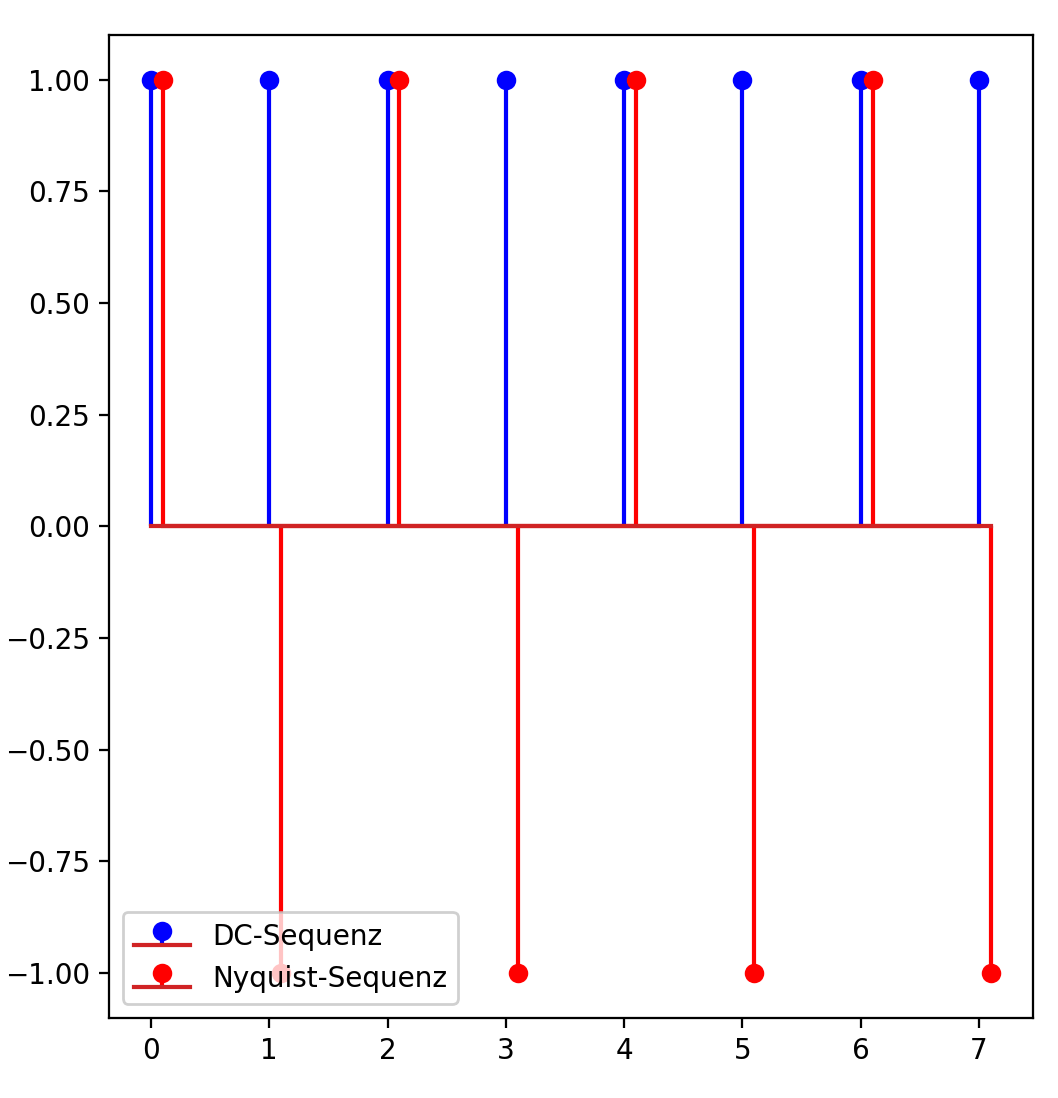
\includegraphics[width=\textwidth]{code/nyquist_seq.png}
    \end{minipage}
    \codecaption{dsv/code/nyquist_seq.py}{Darstellung der DC-Sequenz und der Nyquist-Sequenz f"ur $N=8$}\label{py:nyquist_seq}
\end{listing}

Man in \Cref{py:nyquist_seq} gut, dass die beiden Sequenzen wirklich \q{Gegens"atze} darstellen, da $x_0[\cdot]$ die Anteile mit \q{minimaler} Variation/Frequenz aufsammelt, w"ahrend die Werte von $x_{N/2}[\cdot]$ genau so liegen, dass ein analoges Signal (und dessen Aliase), siehe \Cref{py:aliasing}, genau Frequenz $F_s/2$ (und Amplitude $1$) besitzen muss, um $x_{N/2}[\cdot]$ als Abtastwerte zu erhalten.
%
%
\paragraph{Zyklische Faltung}
%
Kommen wir nun zur wahrscheinlich wichtigsten Eigenschaft der \gls{dft} und dem Grund, warum digitale Signalverarbeitung "uberhaupt erm"oglicht wurde.
Wir haben bereits gesehen, dass \gls{lti}-Systeme durch eine Faltung realisiert werden k"onnen.
Gegeben zwei $N$-periodische Signale $x_{1,2}[\cdot]$ und betrachten wir deren \emph{zyklische} Faltung $\circledast$ definiert durch
\begin{equation}\label{eq:fourier:cyclic_conv}
x_3[m] = \Sum{n=0}{N-1}{x_1[n] \cdot x_2[(m-n) \mod N]} = (x_1 \circledast x_2)[m],
\end{equation}
dann kann man zeigen, dass
\[
X_3[k] = X_1[k] \cdot X_2[k]
\]
gilt.
Das hei"st, dass die zyklische Faltung von zwei periodischen Signalen wieder ein periodisches Signal ergibt, dessen \gls{dft} das Produkt der \glspl{dft} der gefalteten Signale ist.
Wenn wir an \gls{lti}-Systeme denken und uns erinnern, dass viele Filter als \gls{lti}-Systeme aufgefasst werden k"onnen, so ist klar, warum diese Eigenschaft wichtig ist.
Die digitalen Filter k"onnen also im Frequenzbereich sehr einfach angewendet werden, weil dort nur eine einfache punktweise Multiplikation notwendig ist.
Doch dies allein ist nicht ausreichend, denn wir ben"otigen noch einen effizienten weg, um zwischen Zeit- und Freqeunzbereich wechseln zu k"onnen.
Dies wird uns durch die \gls{fft} erm"oglicht werden.
In \Cref{py:dft_1} hatten wir bereits erfahren, dass man die \gls{dft} als Matrix-Vektor-Produkt formulieren kann, wozu etwa \glspl{flop} in der Gr"o"senordnung $N^2$ notwendig sind.
Die \gls{fft} erlaubt es aber eine \gls{dft} mit \glspl{flop} in der Gr"o"senordnung von nur $N \log{N}$ durchzuf"uhren.
%
% \begin{itemize}
%     \item \begin{itemize}
%         \item reelles signal: dc und nyquist reell
%     \end{itemize}
%     \item dft als approximation der dtft
%     \begin{itemize}
%         \item $s(t) = \exp(-t/\tau) \cdot \sin(\omega_0 \cdot t)$, 
%         \item $s(t) = \exp(-(t - \mu)^2/\sigma^2)$ (Uebung)
%     \end{itemize}
% \end{itemize}

%
%
\subsection{Abtastung von Signalen}\label{sampling}
%
\begin{itemize}
    \item uebergang von analog zu digital: 
    \item beispiele: schallwelle zu mikro zu spannung, zu adc, zu WAV; em-welle zu antenne, zu adc, zu IQ samples; licht, durch linse, auf CMOS-sensor, zu RAW
    \item Sampling Rate: ADC samples pro sekunde, CMOS-sensor pixeldichte
    \item Wert-Diskretisierung: ignorieren wir vorerst
\end{itemize}
%
%
\subsection{DFT-Interpolation}\label{dftintp}
%
% !TEX root = ../dsv_script.tex
%
%
\subsubsection{Theoretische Grundlagen}\label{sec:dftintp:theory}
%
Gegeben sei ein periodisches, analoges Signal $x: \R \rightarrow \C$, mit Periode $T_p = 1/F_0$. 
Wir beobachten dieses Signal auf einem uniformen Raster von Punkten, via $x[n] = x(n T)$ und wollen eine Funktion $y(t)$ herleiten, f\"ur welche die Interpolationsbedingung
\begin{equation}\label{eq:dftintp:interpol_cond}
    y(nT) = x[n] = x(nT)
\end{equation}
erf\"ullt ist. 
Hierzu entwickeln wir das Signal $x$ in seine Fourier-Reihe via
\begin{equation}\label{eq:dftintp:fourier_series}
    x(t) = \Sum{k=-\infty}{+\infty}{
        c[k] \exp(\jmath 2 \pi k t F_0) 
    }.
\end{equation}
Nun tasten wir dieses Signal uniform mit Samplerate $F_s = N/T_p = 1/T$ (also passend zur Periodendauer) ab und erhalten die Folge 
\begin{equation}
    x[n] = x(n T) = \Sum{k=-\infty}{+\infty}{
        c[k] \exp(\jmath 2 \pi k n T F_0) 
    } = \Sum{k=-\infty}{+\infty}{
        c[k] \exp\left(\jmath 2 \pi k \frac nN\right) 
    }
    \Text{f\"ur}
    n \in \N
\end{equation}
bestehend aus den Samples von $x$. 
Mit der Periodizit\"at von $\exp(\jmath 2 \pi t)$, siehe \Cref{sec:fourier:disc_period} und \Cref{sec:sampling:disc_sin}, und der Abtastung erhalten wir au{\ss}erdem noch
\begin{equation}
    x[n] = \Sum{k=0}{N-1}{
        \left[\Sum{\ell=-\infty}{+\infty}{
            c[k - \ell N]
        }\right] \exp\left(\jmath 2 \pi k \frac nN\right) 
    } = \Sum{k=0}{N-1}{
        \tilde{c}[k] \exp\left(\jmath 2 \pi k \frac nN\right) 
    },
\end{equation}
wobei wir 
\begin{equation}\label{eq:dftintp:aliased_ck}
    \tilde{c}[k] = \Sum{\ell=-\infty}{+\infty}{
        c[k - \ell N]
    }
\end{equation}
als Abk\"urzung benutzt haben. 
Wir nehmen nun aus guten Grund noch an, dass die Funktion $x$ auch bandbegrenzt ist.
Das hei\"st, ihre Fourier-Transformierte $X : \R \rightarrow \C$ verschwindet au{\ss}erhalb eines gewissen Bandes, also
\begin{equation}
    X(F) = \Int{-\infty}{+\infty}{x(t) \exp(-\jmath 2 \pi F t )}{t} = 0 \Text{f\"ur} \Abs{F} > B.
\end{equation}
Au{\ss}erdem wissen wir, dass die Fourier-Transformation $X$ und die Folge $c[k]$ verkn\"upft sind via 
\begin{equation}
    c[k] = \frac{1}{T_p} X(k F_0),
\end{equation}
was impliziert, dass die Folge $c[k]$ ab einem gewissen $k > K_0$ verschwindet.
Es gilt also
\begin{equation}
    c[k] = 0 \Text{f\"ur} \Abs{k} > \left\lceil \frac{B}{F_0} \right\rceil.
\end{equation}
Das hei{\ss}t, dass wir nun $F_s = N/T_p$ so gro{\ss} w\"ahlen m\"ussen, dass sich in \eqref{eq:dftintp:aliased_ck} kein Aliasing f\"ur $\tilde{c}[k]$ ergeben kann.
Es muss also gelten
\begin{equation}
    N > \lceil B/F_0 \rceil \Text{bzw.} F_s > \lceil B/(F_0 T_p) \rceil.
\end{equation}
Es folgt dann, dass $c[k] = X[k]$, wobei $X[k]$ die \gls{dft} der Folge $x[n]$ darstellt. 
Das hei\"st, dass wir die Fourier-Koeffizienten der kontinuierlichen Funktion $x$ durch die \gls{dft} der Abtastwerte $x[n]$ bestimmen k\"onnen. 
Mit \eqref{eq:dftintp:fourier_series} k\"onnen wir also die Folge $x[n]$ interpolieren, indem wir
\begin{equation}\label{eq:dftintp:dft_interpolation}
    y(t) = \frac{1}{T_p}\Sum{k=-\frac{B}{F_0}}{+\frac{B}{F_0}}{
        X[k] \exp(\jmath 2 \pi k t F_0) 
    }
\end{equation}
schreiben. 
Dieses $y$ erf\"ullt die Interpolationsbedingung \eqref{eq:dftintp:interpol_cond}, weil wegen der Bandbegrenzung von $x$ und der Periodizit\"at sogar $y(t) = x(t)$ f\"ur alle $t$ gilt.

Man beachte hier, dass nun aus der Folge von diskreten Werten $x[n]$ eine analytische Formel in Form einer \emph{endlichen} Summation entstanden ist. 
Unter der Annahme der Bandlimitierung von $x$ ist diese Interpolation \emph{exakt} und kann effizient implementiert werden, durch die Vorberechnung der Folge $X[k]$ durch die \gls{fft}~\cite{FFTW05} der Folge $x[n]$. 
Eine Anwendung der hier vorgestellten Methode zur Interpolation wird in \cref{sec:eadf} aufgezeigt.
%
%
\subsection{Wavelets}\label{wavelets}
%
%
\subsection{B-Splines}\label{bsplines}
%
% !TEX root = ../dsv_script.tex
%
Eine Grundvoraussetzung f"ur eine praktisch n"utzliche digitale Signalverarbeitung ist die M"oglichkeit zwischen dem analogen und digitalen Bereich wechseln zu k"onnen. 
Hierbei sollte man auch genau quantifizieren k"onnen, ob bei diesem Prozess Informationen verloren gehen, oder wie man garantieren kann, dass diese Umwandlung verlustfrei vonstatten geht. 
Meist nutzt man hierf"ur das Sampling \Cref{stm:sampling_theorem}. 
Die hieraus resultierende sogenannte Nyquist-Sampling-Theorie fu"st bekannterma"sen auf der Repr"asentation von bandbegrenzten Signalen durch hinreichend dichte "aquidistante Abtastwerte.

Es gibt jedoch auch einige Nachteile von Nyquist-Sampling, die aus dessen Annahmen und der daraus folgenden Verarbeitung entstehen. 
Einerseits kann ein endliches Signal im Allgemeinen \emph{nicht} bandbegrenzt sein. 
Weiterhin entstehen durch die Bandlimitierung von Signalen Gibbs-Artefakte, siehe \Cref{py:dtft}, die besonders bei der Bilderverarbeitung nicht erw"unscht sind. 
Geht es um die Auswertung $x(t)$ eines Signals $x$ zwischen den aufgenommenen Samples $x[n]$, also um Interpolation, hat man das Problem, dass die $\Sinc$-Funktion nur sehr langsam mit Rate $1/t$ abf"allt.
Diese Eigenschaft f"uhrt dazu, dass man f"ur die Bestimmung eines Wertes $x(t)$ mit einer Genauigkeit von \SI{1}{\percent} etwa $100$ um $t$ benachbarte Samples betrachten muss. 
Das hei"st, vor allem bei 2D-Interpolation, siehe \Cref{sec:dftintp}, skaliert der resultierende Rechenaufwand nicht sehr g"unstig, falls hohe Genauigkeit ben"otigt wird.

Aus diesem Grund m"ochten wir uns eine alternative Sampling-Theorie genauer ansehen -- die B-Splines~\cite{unser1999splines_mag}. 
Wir f"uhren zun"achst die auf Polynomen basierende Signalverarbeitung ein und vergleichen sie anschlie"send zur bereits bekannten Nyquist-Theorie.

\subsection{B-Splines als Polynome}

Allgemein bezeichnet man st"uckweise definierte und stetig differenzierbare Polynome als Splines. 
Man nennt die Stellen an denen zwei unterschiedliche Polynome zusammensto"sen als Knoten. 
Ein Spline der Ordnung $\ell \in \N$ ist ein Polynom vom Grad $\ell$, ist also von der Form
\begin{equation}
    p(t) = 
        a_{\ell} t^{\ell} 
        + a_{\ell - 1} t^{\ell-1} 
        + \dots
        + a_1 t 
        + a_{0}.
\end{equation}
%
Ein Spline ist nun eine Funktion $s(t)$, welche f"ur Knoten $n = 1, 2, \dots$ definiert ist durch
\begin{equation}
    s(t) = \begin{cases}
        p_1(t) \fuer x \in [1,2], \\
        p_2(t) \fuer x \in [2,3], \\
        \vdots
    \end{cases}
\end{equation}
wobei sich die Glattheit durch die Forderung ergibt, dass die Funktion und ihre Ableitungen an den Knoten stetig sei, also
\begin{equation}
    \lim\limits_{t \rightarrow n^-} s^{(m)}(t) =
    \lim\limits_{t \rightarrow n^+} s^{(m)}(t)
\end{equation}
erf"ullt ist, wobei $s^{(m)}$ f"ur $m \geqslant 0$ die $m$-te Ableitung des Splines $s$ repr"asentiert. 
In einer Arbeit~\cite{schoenberg1988bsplines}, die sogar dem ber"uhmten Paper von Shannon vorausgeht, beschreibt Schoenberg, dass sich diese Splines der Ordnung $\ell$ via
\begin{equation}\label{eq:bsplines:summation}
    s(t) = \Sum{k \in \Z}{}{
        c[k] \beta^{\ell}(t - k)
    }
\end{equation}
darstellen lassen. Hierbei ist die Funktion $\beta^\ell: \R \rightarrow \R$ definiert als eine iterierte Faltung einer Rechteck-Funktion via
\begin{equation}
    \beta^\ell = \underbrace{
        \beta^0 \ast \dots \ast \beta^0
    }_{(\ell+1) \Text{mal}}, 
    \Text{wobei}
    \beta^0(t) = \begin{cases}
        1,\quad \Abs{t} < \frac{1}{2} \\
        \frac{1}{2}, \quad \Abs{t} = \frac{1}{2} \\
        0, \Text{sonst.}
    \end{cases}
\end{equation}
In \Cref{fig:bsplines:all_splines} sind die Funktionen $\beta^\ell$ f"ur $\ell = 0, \dots, 3$ dargestellt. 
Man erkennt sehr gut, dass der Grad der Glattheit von der Ordnung des Splines abh"angt und dass die Funktionswerte $\beta^\ell(t)$ f"ur $\Abs{t}>\ell+1/2$ verschwinden. 
Man spricht von Funktionen mit \emph{kompaktem Tr"ager}. 
Das hei"st die Summation in \eqref{eq:bsplines:summation} ist f"ur fixes $t \in \R$ \emph{endlich} und ist auf $\ell+1$ Summanden beschr"ankt!
%
\begin{figure}
    \centering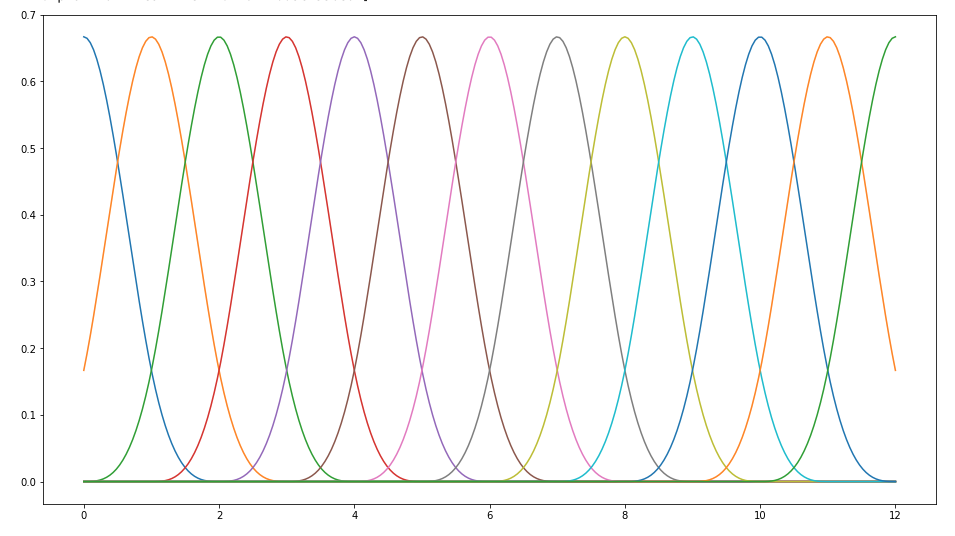
\includegraphics[width=0.9\textwidth]{img/bsplines/all_splines.png}
    \caption{Kubische B-Splines f"ur Abtastung an den Werten $n = 0, \dots, 12$.}\label{fig:bsplines:all_splines}
\end{figure}
%
Wir wollen nun eine explizite Formel f"ur $\beta^\ell$ entwickeln. Hierzu betrachten wir die Fourier-Transformation 
\begin{equation}
    B^\ell(\omega) 
        = \left(\frac{\sin(\omega / 2)}{(\omega / 2)}\right)^{\ell + 1}
        = \frac{(\exp(\jmath \omega/2) - \exp(-\jmath \omega/2))^{\ell+1}}{
            (\jmath \omega)^{\ell + 1}
        }
\end{equation}
mit einigen Rechentricks (siehe \cite[Box 1.]{unser1999splines_mag}) kann man dies so lange umformen, bis man
\begin{equation}
    \beta^\ell(t) = \frac{1}{\ell !}\Sum{p = 0}{\ell+1}{
            \binom{\ell+1}{p}(-1)^p
            \left(t - p + \frac{\ell+1}{2}\right)_+^\ell
        }
    \Text{mit}
    (x)_+ = \begin{cases}
      x, \fuer x \geqslant 0, \\
      0, \Text{sonst},  
    \end{cases}
\end{equation}
erh"alt. 
Damit ist $\beta^\ell$ wirklich ein Polynom $\ell$-ten Grades. 
Die Stetig- und Differenzierbarkeit muss man sich aber noch separat "uberlegen. 

Weiterhin kann man zeigen, dass folgende Formeln f"ur Differentiation und Integration von B-Splines gelten:
\begin{equation}\label{eq:bsplines:deriv_int}
    \left(\beta^\ell\right)^\prime(t) =
        \beta^{\ell-1}(t + 1/2) - \beta^{\ell-1}(t - 1/2), 
    \Int{-\infty}{t}{\beta^\ell(s)}{s} = 
        \Sum{p = 0}{+\infty}{\beta^{\ell+1}(t - 1/2 - p)}.
\end{equation}
Das hei"st, dass man auch einen kompletten Spline $s$ differenzieren und integrieren kann, indem man nutzt, dass sowohl Differentiation, als auch Integration lineare Operationen sind. 
Es gilt also mit \eqref{eq:bsplines:summation} und \eqref{eq:bsplines:deriv_int} beispielsweise f"ur die Differentiation, dass
\begin{equation}
    s^\prime(t) = \Sum{k \in \Z}{}{
        c[k] \left(\beta^{\ell}\right)^\prime(t - k)
    }
    = \Sum{k \in \Z}{}{
        c[k]\left(
            \beta^{\ell-1}(t + 1/2 - k) - \beta^{\ell-1}(t - 1/2 - k)
        \right)
    }.
\end{equation}
%
Diese Eigenschaft macht man sich auch f"ur kompliziertere Operationen, wie Rotationen und Verzerrungen auf einem Spline $s$ zunutze.
%
%
\subsection{Kubische B-Spline Interpolation}
%
%
Wir m"ochten uns eine spezielle Version der B-Splines genauer Ansehen, da diese in der Anwendung den Spagat zwischen Komplexit"at und Approximationsg"ute sehr gut hinbekommen. 
Wir setzen hierzu $\ell=3$ und erhalten somit ein Polynom dritten Grades der Form
\begin{equation}\label{eq:bsplines:explicit_eval}
    \beta^3(t) = \begin{cases}
        \frac 23 - \Abs{t}^2 + \frac{\Abs{t}^3}{2} \fuer \Abs{t} < 1\\
        \frac{(2 - \Abs{t})^3}{6}, \fuer \Abs{t} \in [1, 2) \\
        0, \fuer \Abs{t} > 2,
    \end{cases}
\end{equation}
welche in \Cref{py:bsplines:eval} auch einmal implementiert wurde. 

\begin{listing}
\inputminted[firstline=4]{python}{code/bsplines_eval.py}
\codecaption{dsv/code/bsplines_eval.py}{Implementierung von \eqref{eq:bsplines:explicit_eval}}\label{py:bsplines:eval}            
\end{listing}

In Analogie zum bekannten Nyquist-Sampling wollen wir untersuchen, wie wir aus endlich vielen gegebenen Abtastwerten $x[n]$ mit $n \leqslant N$ eine Darstellung wie in \eqref{eq:bsplines:summation} herleiten k"onnen, welche die abgetasteten Werte exakt interpoliert. Aufgabe ist es also aus $x[n]$ die Folge $c[k]$ zu bestimmen.

Hierzu ben"otigen wir die sogenannte Interpolationsbedingung, siehe \eqref{eq:dftintp:interpol_cond}, welche f"ur eine zu interpolierende Funktion $x$ und ihre Abtastwerte $x[n] = x(n)$ fordert, dass
\begin{equation}\label{eq:bsplines:interpol_cond}
    x(n) = x[n] = s(n) = \Sum{k \in \Z}{}{
        c[k] \beta^{3}(n - k)
    }
\end{equation}
gilt. 
Wir fordern also \emph{exakte} Interpolation. 
Nun k"onnte man f"ur die Bestimmung der Folge $c[k]$ ein lineares Gleichungssystem aufstellen, welches die Form
%
\begin{equation}\label{eq:bsplines:lse}
    \bm B \cdot \bm c = \bm x
\end{equation}
%
hat, wobei die Systematrix $\bm B$ durch die Auswertung der B-Splines an den Stellen $n$ bestimmt ist und der Vektor $\bm x$ den Werten $x[n]$ entspricht. 
Dem endlichen Tr"ager der Funktionen $\beta^\ell$ ist es zu verdanken, dass die Matrix $B$ mit nur wenigen von $0$ verschiedenen Werten besetzt ist (genauer: band-diagonal) und demzufolge effizient invertierbar ist.
Es ist also nicht \q{schwer} $\bm c = \bm B^{-1} \bm y$ zu berechnen. 
Doch die Anwendung von $B^{-1}$ ist numerisch instabil, weshalb wir einen alternativen Weg einschlagen, der auf inverser Filterung beruht.

Sehen wir uns \eqref{eq:bsplines:interpol_cond} genauer an. 
Wir finden, dass sich diese Gleichung nach Definition von $\beta[k] = \beta^3(k)$ als Faltung via
\begin{equation}\label{eq:bsplines:conv}
    x[n] = (c \ast b)[n]
\end{equation}
schreiben l"asst. 
Nach Transformation in den $z$-Bereich erhalten wir
\begin{equation}\label{eq:bsplines:ztrafo}
    X(z) = C(z) \cdot B(z) \Rightarrow C(z) = \frac{X(z)}{B(z)},
\end{equation}
was uns motiviert eine Darstellung von $1/B(z)$ im Zeitbereich herzuleiten. 
F"ur die kubischen B-Splines folgt, dass
\begin{equation}\label{eq:bsplines:filter}
    B(z) = \frac{z + 4 + z^{-1}}{6} 
    \Rightarrow \frac{1}{B(z)} 
        = 6 \left(\frac{1}{1 - z_1 z^{-1}}\right) \left(\frac{-z_1}{1 - z_1 z}\right)
\end{equation}
gilt. 
Wobei man zeigen kann, dass $z_1 = \sqrt{3} - 2 < 1$ gilt. 
Wir betrachten nun $1/B(z)$ als einen Filter, der auf die Abtastwerte $x[n]$ angewandt werden soll. 
Aus \eqref{eq:bsplines:filter} erkennen wir, dass $1/B(z)$ ein Filter ohne Nullstellen ist und als Hintereinanderausf"uhrung von zwei rekursiven Filtern betrachtet werden kann. 
Wir erhalten mit $c^{-}[k] = c[k]/6$, dass sich $1/B(z)$ durch
\begin{align}
    c^+[k] &= 
        x[n] + z_1 c^+[k-1] \fuer k = 1, \dots N-1 \\
    -c[k]/6 = c^-[k] &= 
        z_1\left( c^{-}[k+1] - c^+[k]\right) \fuer k = N-2, \dots, 0
\end{align}
ausdr"ucken l"asst. 
Diese Methode der kausalen und anti-kausalen Filterung ist deutlich effizienter und stabiler, als \eqref{eq:bsplines:lse}, da beispielsweise keine Divisionen notwendig sind. 
Nun ist es noch notwendig Anfangswerte f"ur $c^+[k]$ und $c^-[k]$ zu finden. 
Dies ist aufgrund der Endlichkeit von $x$ nicht ohne Weiteres m"oglich. 
Man sieht, dass die Impulsantwort von $c^+$ eine abklingende Exponentialfunktion ist, also gilt
\begin{equation}
    c^+[0] = \Sum{k=0}{\infty}{x[-k] z_1^k} \approx \Sum{k=0}{K}{x[-k] z_1^k},
\end{equation}
wobei man $K \in \N$ so w"ahlen kann, dass $z_1^K \leqslant \varepsilon$ erf"ullt ist, siehe \Cref{py:exp_mean}.
Nach Ausf"uhrung von $c^+$ kann man $c^-[N-1]$ durch
\begin{equation}
    c^-[N-1] = \frac{z_1}{1 - z_1^2}\left(c^+[N-1] + z_1 c^+[N-2]\right)
\end{equation}
effizient und exakt initialisieren. 
Beides wurde in \Cref{py:bsplines:coeffs} beispielhaft implementiert und eine m"ogliche Ausgabe nach Auswertung von \eqref{eq:bsplines:summation} ist in \Cref{fig:bsplines:interpol} dargestellt.
%
\begin{listing}[t]
\inputminted[firstline=4]{python3}{code/bsplines_coeffs.py}
\codecaption{dsv/code/bsplines_coeffs.py}{Berechnung der B-Spline Koeffizienten}\label{py:bsplines:coeffs}
\end{listing}
%
\begin{figure}[t]
    \centering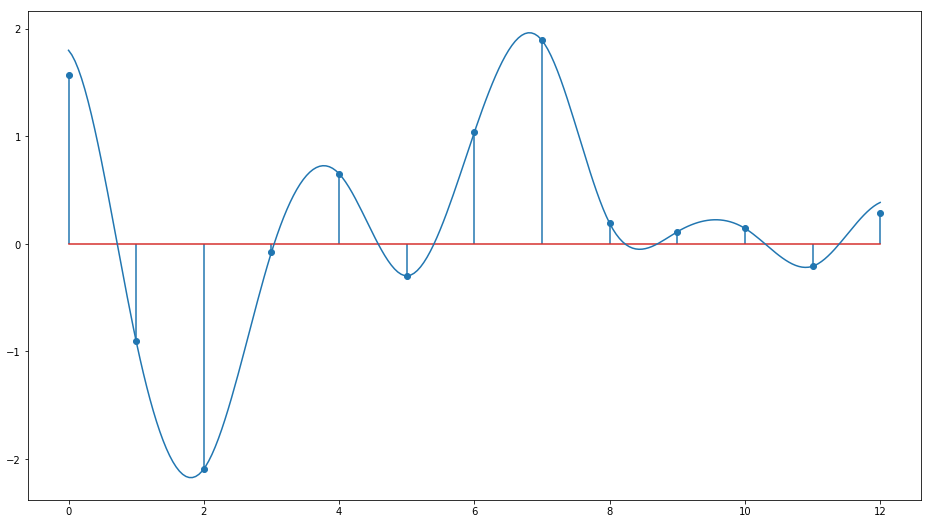
\includegraphics[width=0.9\textwidth]{img/bsplines/interpol.png}
    \caption{Kubische B-Spline-Interpolation f"ur Abtastung an den Werten $n = 0, \dots, 12$.}\label{fig:bsplines:interpol}
\end{figure}
%
%
%
\subsection{Verbindung zur Nyquist-Sampling-Theorie}
%
%
Wir wollen als Abschluss eine Verbindung zum Sampling und der Interpolation~\cite[Kapitel~6.1]{proakis2013} von bandbegrenzten Funktionen mit endlicher Energie ziehen. 
Nehmen wir als Wiederholung zun"achst an, dass das bandbegrenzte Signal $x_a$ mit endlicher Energie und Fourier-Transformation $X_a$ mindestens kritisch mit Rate $F_s$ zu den Werten $x[n]$ abgetastet wurde. 
Wir bezeichnen mit $X$ die \gls{dtft} von $x[n]$. Dann gilt als Zusammenhang zwischen den beiden Spektra, wie in \Cref{sec:sampling:sampling_theorem}, dass
\begin{equation}
    X(f) = F_s \Sum{k=-\infty}{+\infty}{
        X_a((f - k) F_s)
    },
\end{equation}
was die Periodifizierung des Frequenzbereiches durch Abtastung ausdr"uckt. 
Nach Annahme der kritischen Abtastung findet hier kein Aliasing statt, sodass f\u"r $f \in [-F_s/2,+F_s/2]$ gilt, dass $F_s \cdot X_a(f) = X(f)$. 
Au"serdem k"onnen wir das Spektrum der abgetasteten Werte $X$ durch
\begin{equation}
    X(f) = \Sum{n=-\infty}{+\infty}{x[n] \exp(- \jmath 2 \pi f n / F_s)}
\end{equation}
ausdr"ucken. 
Nun k"onnen wir das analoge Signal $x_a$ in Abh"angigkeit von den Abtastwerten darstellen. 
Es gilt mit $T = 1/F_s$ und nach \Cref{stm:sampling_theorem}, dass
\begin{align*}
    x_a(t) = \Sum{n=-\infty}{+\infty}{
        x[n] \frac{\sin(\pi(t-nT)/T)}{\pi(t-nT)/T}
    }.
\end{align*}
Das hei"st, dass die Funktion $g: \R \rightarrow \R$ mit
\begin{equation}\label{eq:bsplines:sinckernel}
    g(t) = \frac{\sin(\pi t / T)}{(\pi t/T)}
\end{equation}
als \emph{Interpolations-Kernel} von bandbegrenzten und abgetasteten Funktionen betrachtet werden kann. 
Siehe \Cref{sec:eadf} f"ur eine Anwendung dieser Art der Interpolation.

Nun k"onnen wir eine analoge Rechnung f"ur die B-Splines durchf"uhren, indem wir einen Filter $b^{-1}[k]$ als inverse $Z$-Transformation von $1/B(z)$ aus \eqref{eq:bsplines:ztrafo} definieren. 
Dann gilt
\begin{equation}
    c[k] = (b^{-1} \ast x)[k],
\end{equation}
was wir in \eqref{eq:bsplines:interpol_cond} einsetzen und dann
\begin{equation}
    s(t) = \Sum{n \in \Z}{}{
        (b^{-1} \ast x)[n] \beta^{\ell}(t - n)
    } = \Sum{n \in \Z}{}{
        x[n] \Sum{p \in \Z}{}{
            b^{-1,\ell}[p] \beta^{\ell}(t - n - p)
        }
    } = \Sum{n \in \Z}{}{
        x[n] h^\ell(t - n)
    }
\end{equation}
erhalten, wobei wir analog zu \eqref{eq:bsplines:sinckernel} den Interpolationskernel $h: \R \rightarrow \R$ durch
\begin{equation}\label{bsplines_kernel}
    h^\ell(t) = \Sum{p \in \Z}{}{
        b^{-1,\ell}[p] \beta^{\ell}(t - p)
    }
\end{equation}
definiert haben. 
Man kann zeigen, dass $\lim_{l \rightarrow \infty} h^\ell = g$. 
Das hei"st, dass die $\Sinc$-Interpolation als Grenzwert der B-Spline Interpolation aufgefasst werden kann -- oder andersherum -- die B-Spline-Interpolation als Approximation der $\Sinc$-Interpolation. 
Das hei"st, dass auch im Frequenzbereich Konvergenz in der Form
\begin{equation}
    H^\ell(\omega) = \left(\frac{\sin(\omega/2)}{\omega/2}\right)^{\ell+1} \frac{1}{B^{\ell}(\exp(\jmath \omega))} \rightarrow_{\ell \rightarrow \infty} \Rect(\omega)
\end{equation} 
gegeben sein muss.

Zusammenfassend kann man sagen, dass B-Splines einen alternativen Zugang zu digitaler Signalverarbeitung bieten, welcher eng mit dem des Nyquist-Samplings verkn"upft ist und als Approximation von diesem gesehen werden kann. 
B-Splines sind wegen ihrer effizienten und stabilen Implementierung sowohl bei der Analyse \eqref{eq:bsplines:filter}, als auch der Synthese \eqref{eq:bsplines:summation} vor allem f"ur hochdimensionale Interpolationen sehr interessant\linkfootnote{https://developer.nvidia.com/gpugems/gpugems2/part-iii-high-quality-rendering/chapter-20-fast-third-order-texture-filtering}.

%
%
\subsection{Zuf\"allige Signale}
%
Bisher waren wir ausschließlich mit deterministischen Signalen befasst. 
Also solchen, welche sich bequem durch eine Funktionsvorschrift $t \mapsto x(t)$ beschreiben lassen.
Doch eigentlich ist dies ein absolut idealisierter Spezialfall, da für gew\"ohnlich alle Signale, die wir verarbeiten, zu mindestens einem Zeitpunkt von einem Messgerät beobachtet wurden.
Somit sind diese notwendigerweise mit Messrauschen behaftet, dessen unangenehme Eigenschaft es ist, zuällig zu sein.
Aus diesem Grund ist es uns nicht m\"oglich, ein gemessenes und digitalisiertes Signal $x[\cdot]$ mittels eines alebraischen Ausdrucks zu beschreiben.
Notwendigerweise wird $x[\cdot]$ zu einer sog. Zufallsgr\"oße, welche wir \q{nur} noch durch deren statistische Eigenschaften beschreiben k\"onnen.
Nicht nur das, auch jede folgende Verarbeitung von $x[\cdot]$, bespielsweise durch ein \gls{lti}-System, wird zu einer Zufallsgr\"oße, deren Eigenschaften u.A. von denen des Messrauschens abhängen.

Weiterhin kann es für gewisse Anwendungen auch absolut ausreichend sein, eigentlich deterministische Signale als zufällig zu modellieren.
Wenn es beispielsweise darum geht, zu bestimmen, ob ein Kommunikationssystem in der Lage ist, Informationen fehlerfrei zu übertragen, dann kann es ausreichend sein, \q{nur} eine Ausfallrate zu bestimmen, oder diese Rate zu begrenzen, anstatt dies für jedes m\"ogliche übertragene Signal zu bestimmen/gewährleisten.

Um diese \q{neue} Sichtweise auf Signale gut verinnerlichen zu k\"onnen, ben\"otigen wir jedoch einige Werkzeuge aus der Wahrscheinlichkeitstheorie, die wir uns nun ansehen werden, wobei wir versuchen, uns nicht mit vielen mathematischen Details aufzuhalten, sondern wollen stattdessen unsere Intuition schärfen.

\subsection{Grundlagen Wahrscheinlichkeitstheorie}\label{sec:random:prbly}

Nehmen wir zunächst einmal an, dass wir einen zufälligen Vorgang betrachten, dessen Ausgang sich in Form einer einzelnen reellen Zahl manifestiert.
Diesen zufälligen Vorgang assoziieren wir mit der Zufallsgr\"oße $X : \Omega \rightarrow \R$, also $\omega \rightarrow X(\omega)$, wobei wir uns vorstellen, dass $\Omega$, beziehungsweise $\omega$, dafür sorgen, dass Zufall ins Spiel kommt. \textit{$\ast$MITHÄNDENWEDEL$\ast$} Wir sind nun daran interessiert, wie die \emph{Verteilung} der Werte $X(\omega)$ charakterisiert werden kann.

Hierzu definieren wir beigeordnet zu $X$ eine Funktion $F_X: \R \rightarrow [0,1]$, welche uns für $x \in \R$ mitteilt, was die Wahrscheinlichkeit für das Ereignis $X \leqslant x$ ist.
Man kann auch sagen/schreiben:
\[
F_X(x) = P(X \leqslant x).
\]
Die Funktion $F$ ist monoton wachsend, da natürlich $P(X \leqslant x_1) \leqslant P(X \leqslant x_2)$, falls $x_1 < x_2$, also auch $F_X(x_1) \leqslant F_X(x_2)$.
Jetzt kann man mit der \emph{Verteilungsfunktion} $F_X$ schon eine Menge anfangen.
Beispielsweise k\"onnen wir damit auch bestimmen, mit welcher Wahrscheinlichkeit das Ereignis $x_1 < X \leqslant x_2$ eintritt, indem wir einfach 
\[
P(x_1 < X \leqslant x_2) = F_X(x_2) - F_X(x_1)
\]
berechnen.

Wir k\"onnen sogar noch einen Schritt weiter gehen, und die Gr\"oße
\[
f^h_X(x) = \frac{F_X(x + h) - F_X(x)}{h}
\]
betrachten.
Man kann es sich so vorstellen, dass wir das Intervall $[x,x+h]$ hernehmen, berechnen, wie \q{viel} von $X$ in $[x,x+h]$ landen kann, und normieren das mit der Intervallbreite $h$.
Im Grunde berechnen wir, wie \q{dicht} die Zufallsgr\"oße zwischen $x$ und $x+h$ ist.
Aus diesem Grund nennt man
\[
f_X(x) = \lim\limits_{h \rightarrow 0} f^h_X(x) = \lim\limits_{h \rightarrow 0} \frac{F_X(x + h) - F_X(x)}{h}
\]
die \emph{Dichte} von $X$.
Natürlich sehen wir, dass der berechnete Grenzwert der sogenannte Differenzenquotient der Verteilungsfunktion $F_x$ ist. Es gilt also $f_X = F^\prime_X$.
Deshalb kann man nun die Verteilungsfunktion auch aus der Dichte gewinnen, indem wir
\[
F_X(x) = \Int{-\infty}{x}{f_X(s)}{s}
\]
auswerten.
Die obigen Betrachtungen gelten freilich nur, wenn die formulierten Grenzwerte auch immer existieren, doch erstens existieren diese meistens und für ein intuitives Verständnis sollte es zunächst genügen.

Weiterhin gilt für reelle Zufallsgrößen $X$, dass diese sich \q{irgendwo} zwischen $-\infty$ und $+\infty$ mit Wahrscheinlichkeit $1$ realisieren muss.
Also gilt
\[
\lim_{x \rightarrow \infty} F_X(x) = 1,
\]
was für die Dichte ergibt, dass
\[
\Int{-\infty}{+\infty}{f_X(s)}{s} = 1.
\]
%
%
\subsubsection{Beispiele}
%
\paragraph{Uniforme Verteilung/Gleichverteilung}
Gegeben zwei reelle Zahlen $a < b$ nennt man eine Zufallsgröße $X$ verteilt nach $\Unif(a,b)$, wenn die Dichte $f_X$ gegeben ist durch
\[
f_X(x) = \begin{cases}
    0, \Text{falls} x<a, \\
    1/(b-a), \Text{falls} a \leqslant x < b \\
    0, \Text{falls} b \leqslant x.
\end{cases} = 
    \frac 1{b-a} \Rect\left(\frac{x-(b+a)/2}{b-a}\right)
\]
Der Name dieser Verteilung ergibt sich daraus, dass intuitiv alle Intervalle, die im Intervall $[a,b]$ liegen mit einr Wahrscheinlichkeit proportional zu ihrer \q{Länge} von $X$ \q{getroffen} werden.
Man schreibt auch oft $X \sim \Unif(a,b)$.
%
\paragraph{Normalverteilung}
Gegeben zwei Parameter $\mu \in \R$ und $\sigma^2 \in \R^+$, so nennt man eine Zufallsgröße $X$ normalverteilt mit Erwartungswert $\mu$ und Varianz $\sigma^2$, falls deren Dichte $f_X$
\[
f_X(x) = \frac{1}{\sqrt{2 \pi \sigma^2}} \exp\left(-\frac{(x - \mu)^2}{2 \sigma^2}\right)
\]
erfüllt.
Die Normalverteilungist eine sehr wichtige Verteilung, weil aus Gründen die meisten Messwerte einer Normalverteilung mit Erwartungswert $\mu$ und einer gewissen Varianz $\sigma^2$ folgen.
Je größer $\sigma^2$, desto stärker ist die Streuung der gemessenen Werte um den Erwartungswert $\mu$.
Man schreibt auch $X \sim \mathcal{N}(\mu, \sigma^2)$.
Es sind zwei Beispiele in \Cref{py:random:normal1} zusammen mit der Berechnung der Dichte via \texttt{scipy} dargestellt.
Auch hier ist es wieder ratsam, keine eigenen Implementierungen solcher Standardfunktionen zu nutzen und stattdessen auf Funktionen aus getesteten Paketen zurück zu greifen.
\begin{listing}[ht]
    \noindent
    \begin{minipage}{0.51\textwidth}
        \strut\vspace*{-\baselineskip}\newline
        \inputminted[firstline=3, lastline=10]{python3}{code/random/normal1.py}
    \end{minipage}%
    \begin{minipage}{0.48\textwidth}
        \strut\vspace*{-\baselineskip}\newline
        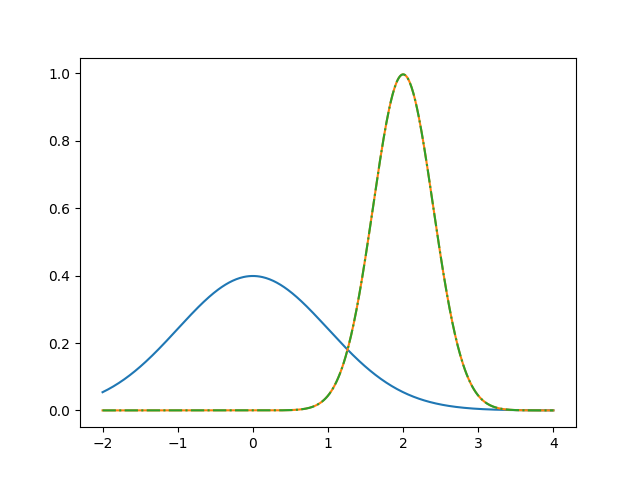
\includegraphics[width=\textwidth]{code/random/normal1.png}
    \end{minipage}
    \codecaption{dsv/code/random/normal1.py}{Visualisierung der Dichte der Normalverteilung für verschiedene Parameter}\label{py:random:normal1}
\end{listing}
%
%
\paragraph{Exponentialverteilung}
Gegeben eine Intensität $\lambda > 0$, so folgt eine Zufallsgröße $X$ einer Exponentialverteilung $\Exp(\lambda)$, falls die Dichte $f_X$ die Form 
\[
f_X(x) = \begin{cases}
    \lambda \exp(-\lambda x), \Text{für} x \geqslant
    0, \\
    0 \Text{sonst}
\end{cases}
\]
besitzt.
Auch eine wichige Verteilung, die beispielsweise die Lebensdauer von irgendwelchen Bauteilen modelliert, oder auch die Wartezeit zwischen zwei Anrufen bei einer Servicehotline. 
Je kleiner $\lambda$, desto höher die Intensität, also desto kürzer die Wartezeit.
%
%
\subsubsection{Erwartungswert, Varianz, Kovarianz}

Will man eine Zufallsgröße auf einige wenige Kennzahlen herunterbrechen, die in der Praxis auch relevant sein könnten, so bieten sich sogenannte Momente deren Verteilung an.
%
%
\paragraph{Erwartungswert}
Interessiert man sich für den Wert, der sich \q{im Mittel} bei einer Verteilung $X$ ergibt, so berechnet man den Erwartungswert $\E(X)$ definiert durch
\begin{equation}\label{eq:random:mean}
    \E(X) = \Int{-\infty}{+\infty}{x f_X(x)}{x}.
\end{equation}
Wenn $f_X$ einer physikalischen Dichteverteilung im Raum entspräche, so würde $\E(X)$ genau den Masseschwerpunkt dieser Verteilung darstellen.
Ist beispielsweise $X \sim \Unif(a,b)$, so gilt $\E(X) = (a+b)/2$ und falls $X \sim \mathcal{N}(\mu, \sigma^2)$, so gilt $\E(X) = \mu$.
%
%
\paragraph{Varianz}
%
Basierend auf dem Erwartungswert, können wir auch die erwartete Streuung einer Zufallsgröße um $\E(X)$ herum betrachten, also
%
\begin{equation}\label{eq:random:var}
\Var(X) 
    = \E((X - \E(X))^2) 
    = \Int{-\infty}{+\infty}{(x-\E(X))^2 f_X(x)}{x}
    = \E(X^2) - \E(X)^2.
\end{equation}
%
Die Interpretation ist, dass $\Var(X)$ die mittlere quadratische Abweichung einer Zufallsgröße von ihrem Erwartungswert beschreibt.
Es ist anzumerken, dass es Verteilungen gibt, für welche $\E$ und $\Var$ nicht existieren müssen, weil die jeweiligen Integrale in \eqref{eq:random:mean} und \eqref{eq:random:var} nicht endlich sind.

Beispielsweise gilt im Falle von $X \sim \Unif(a,b)$, dass $\Var(X) = (b-a)^2/12$ und im Falle von $X \sim \mathcal{N}(\mu, \sigma^2)$, dass $\Var(X) = \sigma^2$.

\subsection{Zufällige Signale}

% - Stochastische Prozesse: definition, zwei sichtweisen (per pfad, folge von verteilungen)
% - stationaere prozesse/signale
% - Wiener-Chintschin-Theorem

\subsection{Parameterschätzung}\label{sec:random:paramest}

\subsection{Quantisierung}\label{sec:random:quanti}

% - \cite{widrow2008quantization}
% - area sampling (geoemetrisch)
% - charakteristische funktion: value at 0, conj sym, 
% - areasampling: analytisch in value domain, in frequ domain
% - reconstruction der PDF aus der quantisierten PDF
% - PQN Model
%
%
\section{Anwendungen}
%
%
\subsection{Radar}\label{radar}
%
%
\subsection{DFT-Interpolation von Antennenantworten}\label{eadf}
%
% !TEX root = ../dsv_script.tex
%
\subsubsection{Motivation}
%
%
Mit jeder Erschlie{\ss}ung von neuen Frequenzbereichen f\"ur die Kommunikation ist es von Interesse das Ausbreitungsverhalten der Elektro-Magnetischen Wellen f\"ur verschiedene Umgebungen zu charakterisieren, beispielsweise innerst\"adtisch, auf der Autobahn, etc. Zwar k\"onnen solche Umgebungen auch computerbasiert simuliert werden, doch f\"ur eine empirisch abgeleitete Statistik solcher sogenannter Kanalmodelle~\cite{delgaldo2007phd} sind repr\"asentative Messungen unerl\"asslich. Diese Charakteristiken werden genutzt, um in realistischen Szenarien Kanalkapazit\"aten, Datenraten und dergleichen zu bestimmen. Schlussendlich flie{\ss}en solche Statistiken dann in neue Mobilfunkstandards ein.

\begin{figure}
    \centering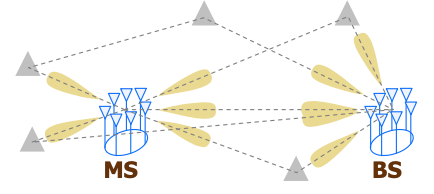
\includegraphics[width=0.6\textwidth]{img/eadf/sounding.png}
    \caption{Schematische Darstellung einer \acrshort{mimo} Kanalmessung. Grafik aus~\cite{richter_estimation_2005}.}\label{eadf_sounding}
\end{figure}

Das FG EMS hat sich deshalb unter anderem auf solche Messungen und deren Auswertung, das sog. Channel Sounding~\cite{thomae2005multidim_hrpe}, spezialisiert. Hierbei kommen meist breitbandige \gls{mimo} Messsysteme zum Einsatz, die den Funkkanal in Frequenz, Raum und Zeit koh\"arent vermessen k\"onnen, wie in \Cref{eadf_sounding} dargestellt. Anschlie{\ss}end nutzt man spezielle Signalverarbeitungstechniken~\cite{semper2023wideband_channel_sounding}, die einerseits unter gewissen physikalischen Annahmen das Ausbreitungsverhalten aus den gemessenen Daten ableiten k\"onnen, und andererseits gleichzeitig den Einfluss des Messsystems so weit wie m\"oglich aus den gesch\"atzten Kanalstatistiken entfernen. Schlie{\ss}lich ist man an der Realit\"at au{\ss}erhalb des Messaufbaus interessiert. 

Nat\"urlich sind hierzu vor der Messung pr\"azise Kalibriermessungen des Systems notwendig. Wir wollen uns im folgenden auf die Wirkung der benutzten Antennenarrays konzentrieren, da diese -- wie wir sehen werden -- eine gewisse Sonderbehandlung ben\"otigen. Zun\"achst stellt man bei der Konzipierung und Benutzung des Messsystems sicher, dass es sich um ein \gls{lti} System handelt. Betrachtet man nun das Verhalten des Systems im Frequenzbereich f\"ur ein einzelnes Paar von Sende- und Empfangsantenne, dann gilt demnach zun\"achst
\begin{equation}
    Y(f) = G_{\rx}(f) \cdot H(f) \cdot G_{\tx}(f) \cdot X(f).
\end{equation}
Hierbei steht $X$ f\"ur die Anregung des Systems durch ein eingegebenes Signal, $G_{\tx/\rx}$ f\"ur die Transferfunktion der Sender- bzw. Empf\"angerhardware, und $H$ f\"ur die Transferfunktion des Funkkanals, der demnach auch als ein \gls{lti} system modelliert wird. Es stellt sich aber heraus, dass jede Antenne eine \emph{winkelabh\"angige} Richtcharakteristik besitzt. Das hei{\ss}t, dass die Systemantworten $G_{\tx/\rx}$ davon abh\"angig sind, in welche Richtungen sich die Wellen vom Sender $\tx$ ausbreiten und aus welchen Richtungen, sie am Empf\"anger $\rx$ eintreffen. 

Um dies korrekt zu modellieren, muss man sich also zun\"achst auf einzelne sog. \emph{Ausbreitungspfade} konzentrieren. Das hei{\ss}t wir nehmen an, dass eine ebene Welle sich in die normierte Richtung $\Omega_{\tx}$ ausbreitet und nach ihrem Weg durch den Funkkanal am Empf\"anger aus normierter Richtung $\Omega_{\rx}$ eintrifft. Folglich ergibt sich f\"ur dieses Verhalten
\begin{equation}\label{eadf_single_path}
    Y(f, \Omega_{\tx}, \Omega_{\rx}) = 
        G_{\rx}(f) \cdot a_{\rx}(f, \Omega_{\rx})
        \cdot H(f, \Omega_{\tx}, \Omega_{\rx}) 
        \cdot a_{\tx}(f, \Omega_{\tx}) \cdot G_{\tx}(f)
        \cdot X(f),
\end{equation}
%
wobei $a_{\tx/\rx}$ f\"ur die richtungs- und frequenzabh\"angige Antwort der Sende- und Empfangsantenne stehen. In diesem Fall bezeichnet also $H(f, \Omega_{\tx}, \Omega_{\rx})$ die Transferfunktion eines einzelnen Pfades, der den Sender in Richtung $\Omega_{\tx}$ verl\"asst und am Empf\"anger aus Richtung $\Omega_{\rx}$ eintrifft. Das hei{\ss}t, wir haben in diesem Fall das Verhalten der Antennen vom Rest des Systems isoliert. 

Die Transferfunktion f\"ur die gesamte Messung wird dann als Summe der Transferfunktionen solcher ebenen Wellen modelliert, also via
\begin{equation}
    Y(f) = \Sum{s = 1}{S}{
        Y(f, \Omega_{\tx,s}, \Omega_{\rx,s})
    },
\end{equation}
was sich dadurch rechtfertigt, dass die Transferfunktion des Kanals sich aus der L\"osung einer partiellen Differentialgleichung ergibt, deren L\"osungsraum lineare Struktur hat.
Es zeigt sich aus \eqref{eadf_single_path}, dass wir eine m\"oglichst pr\"azise Formulierung f\"ur $a_{\tx/\rx}$ ben\"otigen, um die Transferfunktion des Kanals $H$ korrekt bestimmen zu k\"onnen.
%
%
%
\subsubsection{Messvorgang}
%
%
Es ist also unsere Aufgabe f\"ur eine gegebene Antenne ein parametrisches Modell $a: [0, \pi] \times [0, 2\pi] \rightarrow \C$ der Form $a(\varphi, \vartheta) \in \C$, also in Betrag und Phase, herzuleiten. Aus Gr\"unden der Einfachheit und der Physik vernachl\"assigen wir die Frequenzabh\"angigkeit der Antenne und konzentrieren uns auf ihr Verhalten f\"ur die Anregung mit einer einzelnen Frequenz. Auch die Polarisation von ebenen Wellen und das davon abh\"angige Verhalten einer Antenne vernachl\"assigen wir hier. Wir konzentrieren uns also auf die \emph{Winkelabh\"angigkeit} der Antennenantwort.

Wie oben motiviert ben\"otigen wir eine kontinuierliche Beschreibung der Antennenantwort. Doch diese ist uns wegen endlichem Speicherplatz auf Festplatten und angepeilter endlicher Messzeit nicht direkt zug\"anglich. Man wei{\ss} jedoch, dass es einen Zusammenhang zwischen der elektrischen Gr\"o{\ss}e einer Antenne und deren winkelabh\"angigen Verhalten gibt~\cite[Kapitel~4]{delgaldo2007phd}. Das hei{\ss}t, man kann zeigen, dass die Funktion $a$ \emph{bandbegrenzt} ist, beziehungsweise sich sehr gut durch eine bandbegrenzte Funktion \emph{approximieren} l\"asst. Weiterhin ist durch die Stetigkeit der Physik jede Antennencharakteristik periodisch. \emph{$\ast$Fourier-Reihen-Sound intensifies$\ast$}

\begin{figure}[t]
    \centering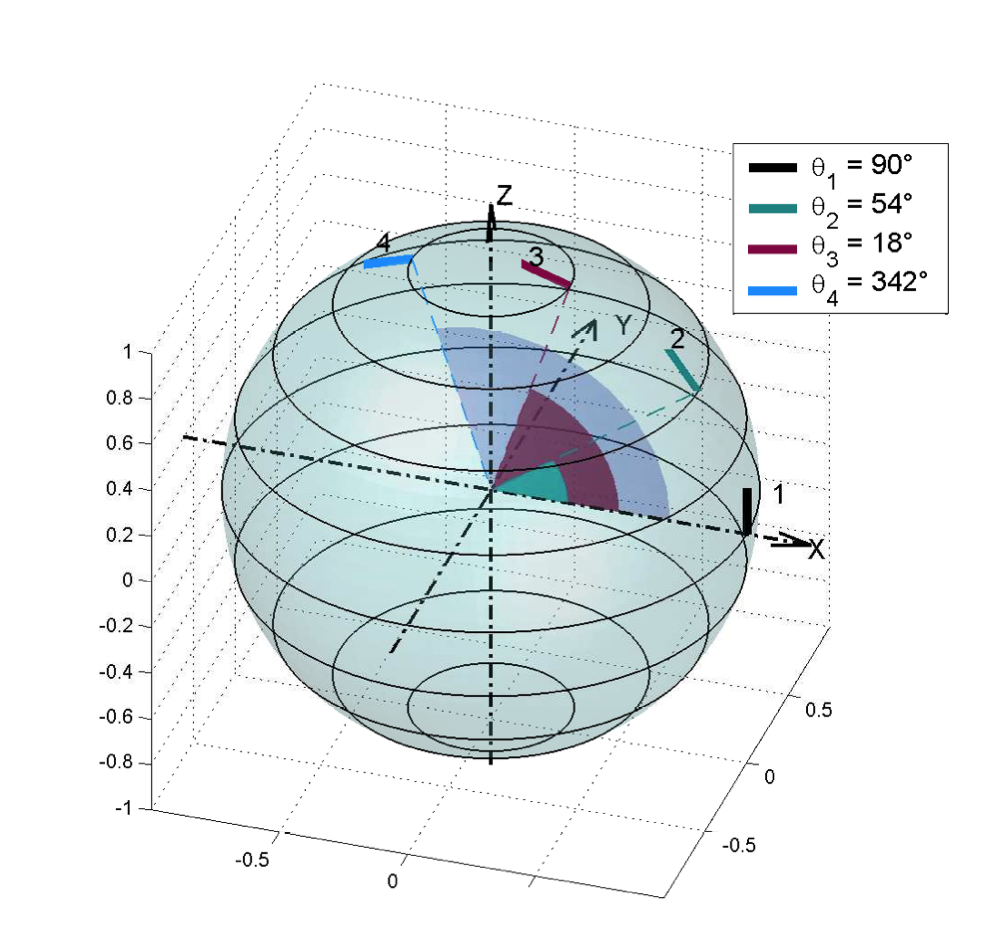
\includegraphics[width=0.49\textwidth]{img/eadf/measure.png}
    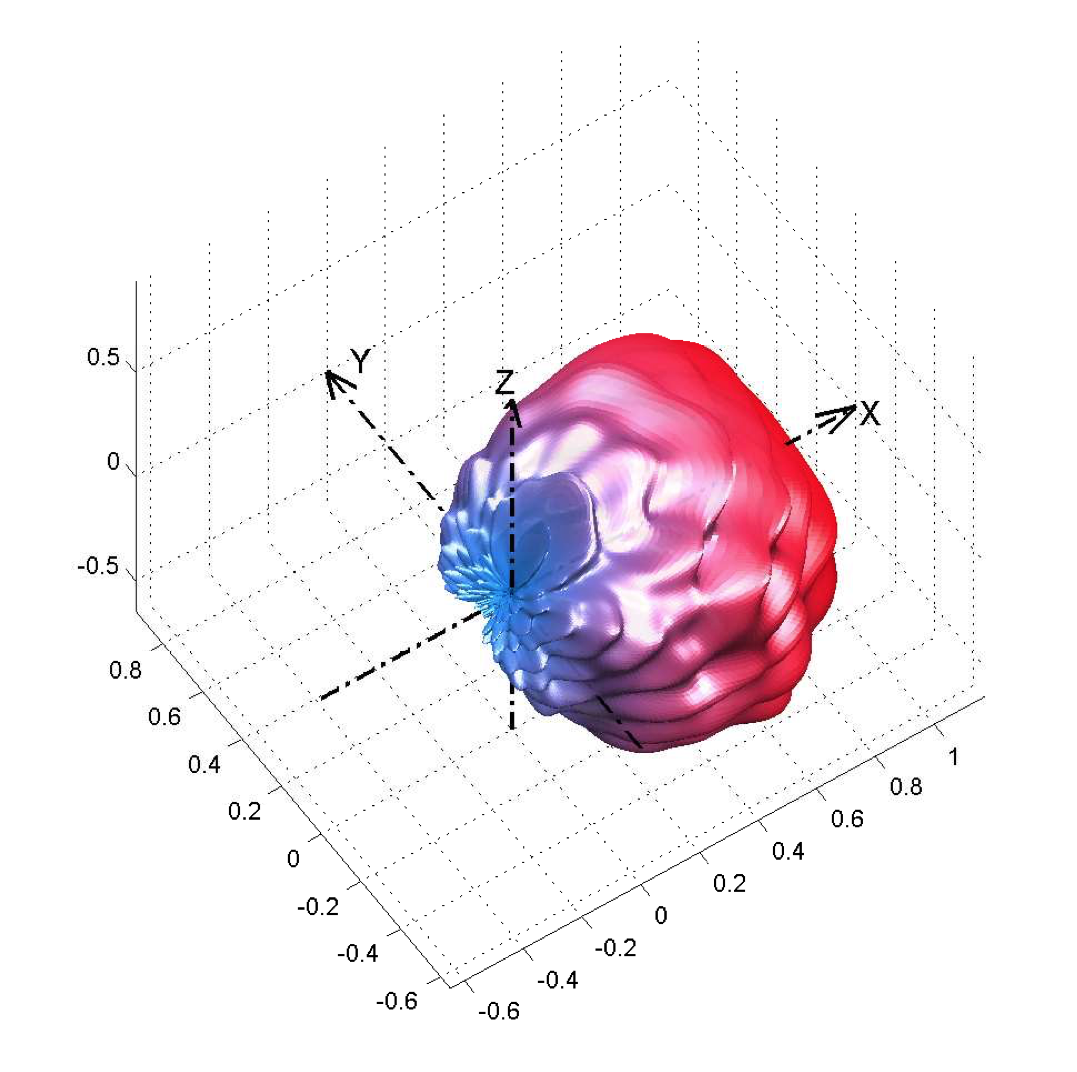
\includegraphics[width=0.49\textwidth]{img/eadf/3d_bp.png}
    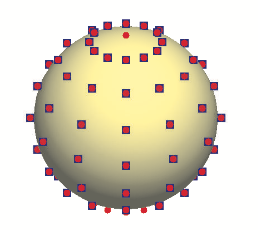
\includegraphics[width=0.3\textwidth]{img/eadf/bp_sampling.png}
    \caption{Links Oben: Darstellung der Messpositionen f\"ur eine Antenne, oder eine Antennenstruktur, welche sich im Ursprung des abgebildeten Koordinatensystems befindet. Rechts Oben: Darstellung der winkelabh\"angigen Amplitude eines einzelnen Patch-Elements. Unten: Messpunkte f\"ur die Abtastung der Funktion $a$. Grafiken aus \cite{landmann2004EADF,delgaldo2007phd}.}\label{eadf_meas}
\end{figure}

Das hei{\ss}t weiterhin, dass es uns m\"oglich ist, die Antenne an diskreten Stellen abzutasten, sodass wir mit der Annahme der Bandbegrenzung und der Aussage des Nyquist-Theorems ein Modell ableiten k\"onnen, welches die Antenne vollst\"andig charakterisiert. In diesem Sinne geht es darum die kontinuierliche Antennenantwort $a$ zu ``digitalisieren''. Die ``Abtastung'' erfolgt demnach im Winkelbereich. Der zugeh\"orige ``Frequenzbereich'' ist entsprechend der \emph{r\"aumliche Frequenzbereich}. \Cref{eadf_meas} zeigt einerseits schematisch den Messaufbau, das genutzte Koordinatensystem und beispielhaft die 3D-Darstellung einer Antennenantwort eines einzelnen Patch-Elements.

Die Messung selbst erfolgt in einer echofreien Messkammer, in welcher es m\"oglich ist, die \gls{aut} beliebig relativ zu einer bereits kalibrierten Referenzantenne zu verdrehen, sodass ein Abtastraster, wie in \Cref{eadf_meas} unten gezeigt, entsteht. Pro Ausrichtung wird die \gls{aut} f\"ur gew\"ohnlich f\"ur mehrere Frequenzen, zwei orthogonale Polarisationen und alle ihre Elemente vermessen, bevor die n\"achste Ausrichtung angefahren wird. Wie erw\"ahnt konzentrieren wir uns auf eine einzelne Frequenz, ein einzelnes Element und eine seiner Polarisationen.
In \Cref{eadf_anechoic} sieht man den Messaufbau, der von unserem FG benutzt wurde, um ein Antennenarray mit 32 Elementen zu vermessen.

\begin{figure}[t]
    \centering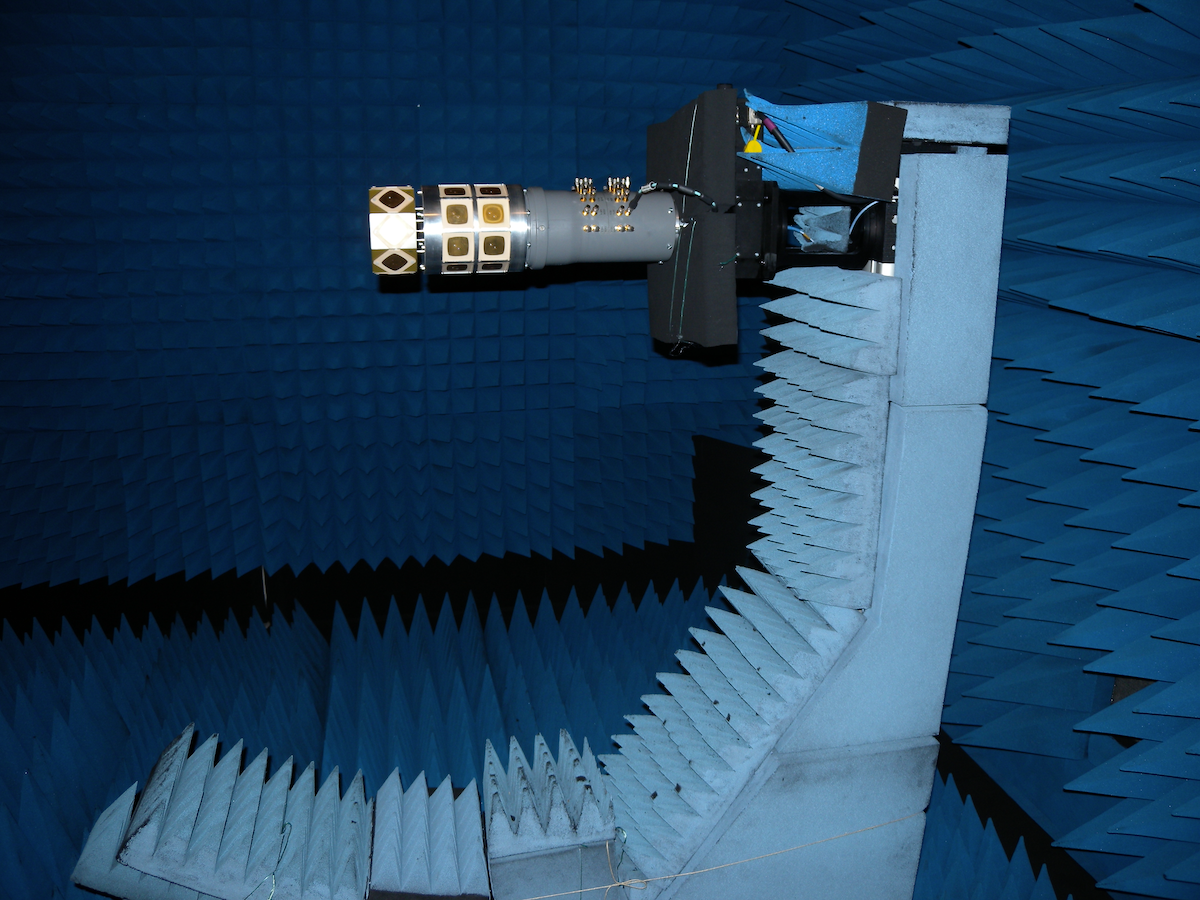
\includegraphics[width=0.49\textwidth]{img/eadf/anechoic1.png}
    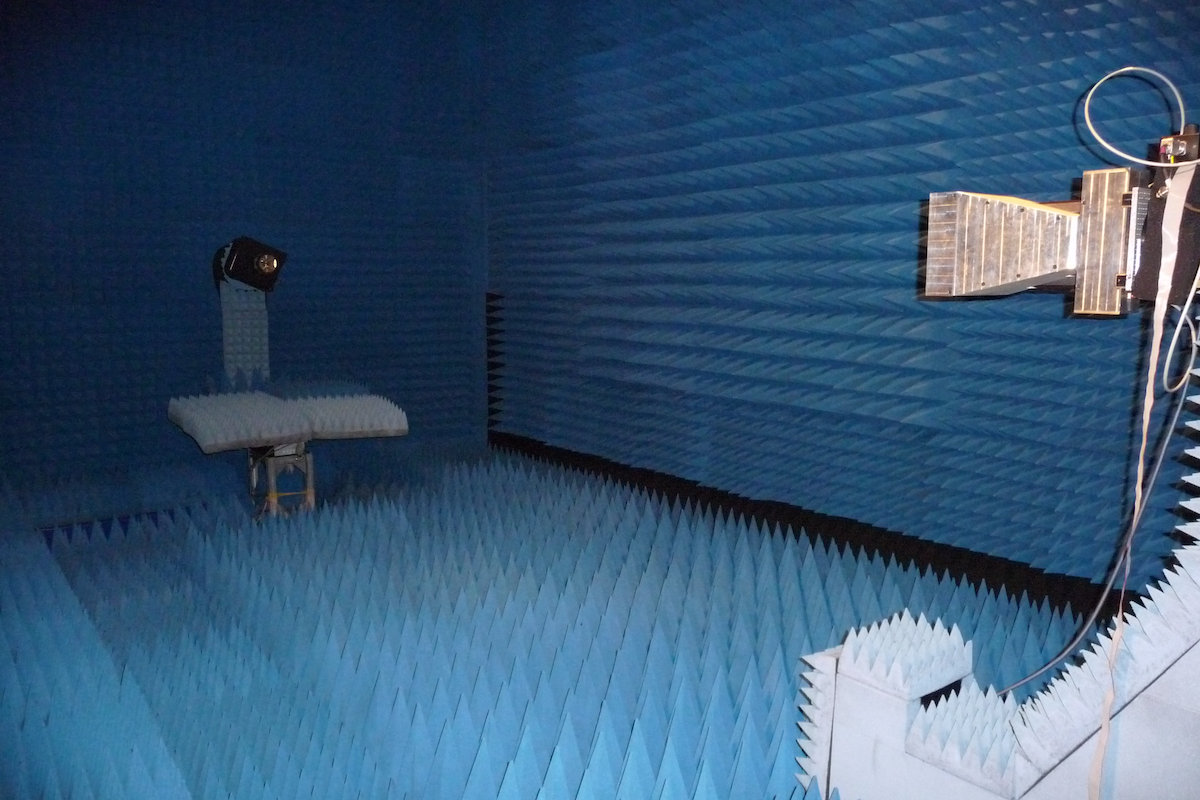
\includegraphics[width=0.49\textwidth]{img/eadf/anechoic2.png}
    \caption{Messaufbau zur Kalibrierung eines Antennenarrays. Links: Drehteller f\"ur die Positionierung der \gls{aut}. Rechts: Weiterer Blickwinkel mit Referenzantenne.}\label{eadf_anechoic}.
\end{figure}

F\"ur ein einzelnes Antennenelement beobachten wir also die Funktion $a$ auf einem Gitter, das aus allen Kombinationen der Punkte 
\[
    \varphi_0, \dots, \varphi_{N_\varphi}, \varphi_i = \frac{i \pi}{N_\varphi}
    \Text{und}
    \vartheta_0, \dots, \vartheta_{N_\vartheta-1}, \vartheta_j = \frac{j 2 \pi}{N_\vartheta}
\]
besteht. Wir erhalten also ein zweidimensionales Array $a[i,j] \in \C^{N_\varphi \times N_\vartheta - 1}$, welches wir noch durch einen Trick geeignet periodifizieren m\"ussen, wie in \cref{eadf_bp_aperture} links dargestellt. Diese Abtastwerte entspringen also einer zweidimensionalen bandbegrenzten, periodischen Funktion. Aufgabe ist es nun aus diesen Werten eine geeignete Interpolante herzuleiten, die sich diese beiden Eigenschaften zunutze macht.
%
%
\subsubsection{Fourier-Interpolation}
%
%
Gegeben sei ein periodisches, analoges Signal $x: \R \rightarrow \C$, mit periode $T_p = 1/F_0$. Wir beobachten dieses Signal auf einem uniformen Raster von Punkten, via $x[n] = x(n T)$ und wollen eine Funktion $y(t)$ herleiten, f\"ur welche die Interpolationsbedingung
\begin{equation}\label{eadf_interpol_cond}
    y(nT) = x[n] = x(nT)
\end{equation}
erf\"ullt ist. Hier zu entwickeln wir das Signal $x$ in seine Fourier-Reihe via
\begin{equation}\label{fourier_series}
    x(t) = \Sum{k=-\infty}{+\infty}{
        c[k] \exp(\jmath 2 \pi k t F_0) 
    }.
\end{equation}
Nun tasten wir dieses Signal uniform mit Samplerate $F_s = N/T_p = 1/T$ (also passend zur Periodendauer) ab und erhalten die Folge 
\begin{equation}
    x[n] = x(n T) = \Sum{k=-\infty}{+\infty}{
        c[k] \exp(\jmath 2 \pi k n T F_0) 
    } = \Sum{k=-\infty}{+\infty}{
        c[k] \exp\left(\jmath 2 \pi k \frac nN\right) 
    }
    \Text{f\"ur}
    n \in \N
\end{equation}
bestehend aus den Samples von $x$. Mit der Periodizit\"at von $\exp(\jmath 2 \pi t)$ und der Abtastung erhalten wir au{\ss}erdem noch
\begin{equation}
    x[n] = \Sum{k=0}{N-1}{
        \left[\Sum{\ell=-\infty}{+\infty}{
            c[k - \ell N]
        }\right] \exp\left(\jmath 2 \pi k \frac nN\right) 
    } = \Sum{k=0}{N-1}{
        \tilde{c}[k] \exp\left(\jmath 2 \pi k \frac nN\right) 
    },
\end{equation}
wobei wir 
\begin{equation}\label{aliased_ck}
    \tilde{c}[k] = \Sum{\ell=-\infty}{+\infty}{
        c[k - \ell N]
    }
\end{equation}
als Abk\"urzung benutzt haben. Ist nun die Funktion $x$ auch bandbegrenzt, d.h.~ihre Fourier-Transformierte $X : \R \rightarrow \C$ verschwindet au{\ss}erhalb eines gewissen Bandes, also
\begin{equation}
    X(F) = \Int{-\infty}{+\infty}{x(t) \exp(-\jmath 2 \pi F t )}{t} = 0 \Text{f\"ur} \Abs{F} > B.
\end{equation}
Au{\ss}erdem wissen wir, dass die Fourier-Transformation $X$ und die Folge $c[k]$ verkn\"upft sind via 
\begin{equation}
    c[k] = \frac{1}{T_p} X(k F_0),
\end{equation}
was impliziert, dass die Folge $c[k]$ verschwindet, also gilt
\begin{equation}
    c[k] = 0 \Text{f\"ur} \Abs{k} > \frac{B}{F_0}.
\end{equation}
Das hei{\ss}t, dass wir nun $F_s = N/T_p$ so gro{\ss} w\"ahlen m\"ussen, dass sich in \eqref{aliased_ck} kein Aliasing f\"ur $\tilde{c}[k]$ ergeben darf. Es muss also gelten
\begin{equation}
    N > \lceil B/F_0 \rceil \Text{bzw.} F_s > \lceil B/(F_0 T_p) \rceil.
\end{equation}
In diesem Falle gilt, dann dass $c[k] = X[k]$, wobei $X[k]$ die \gls{dft} der Folge $x[n]$ darstellt. Das hei{\ss}, dass wir die Fourier-Koeffizienten der kontinuierlichen Funktion $x$ durch die \gls{dft} der Abtastwerte $x[n]$ bestimmen k\"onnen. Mit \eqref{fourier_series} k\"onnen wir also die Folge $x[n]$ interpolieren, indem wir
\begin{equation}\label{dft_interpolation}
    y(t) = \frac{1}{T_p}\Sum{k=-\frac{B}{F_0}}{+\frac{B}{F_0}}{
        X[k] \exp(\jmath 2 \pi k t F_0) 
    }
\end{equation}
schreiben. Dieses $y$ erf\"ullt die Interpolationsbedingung \eqref{eadf_interpol_cond}, weil wegen der Bandbegrenzung von $x$ und der Periodizit\"at sogar gilt $y(t) = x(t)$ f\"ur alle $t$ gilt.

Man beachte hier, dass nun aus der Folge von diskreten Werten $x[n]$ eine analytische Formel in Form einer \emph{endlichen} Summation entstanden ist. Unter der Annahme der Bandlimitierung von $x$ ist diese Interpolation \emph{exakt} und kann effizient implementiert werden, durch die Vorberechnung der Folge $X[k]$ durch die \gls{fft}~\cite{FFTW05} der Folge $x[n]$. 
%
%
%
%
\subsubsection{Ableitung der EADF}
%
%
Wir wollen nun \eqref{dft_interpolation} auf zwei Dimensionen erweitern und folgen damit effektiv~\cite{landmann2004EADF}.
Au{\ss}erdem \"andern wir das Argument der Funktion $x$ und deren Namen zu der oben eingef\"uhrten Schreibweise $a : [0, 2 \pi] \times [0, 2 \pi] \rightarrow \C$ mit Werten $a(\varphi, \vartheta)$. 
In unserem Fall der Interpolation von Antennenantworten wissen wir, dass $a$ in \emph{beiden} Argumenten $2\pi$-periodisch ist.

\begin{figure}[t]
    \centering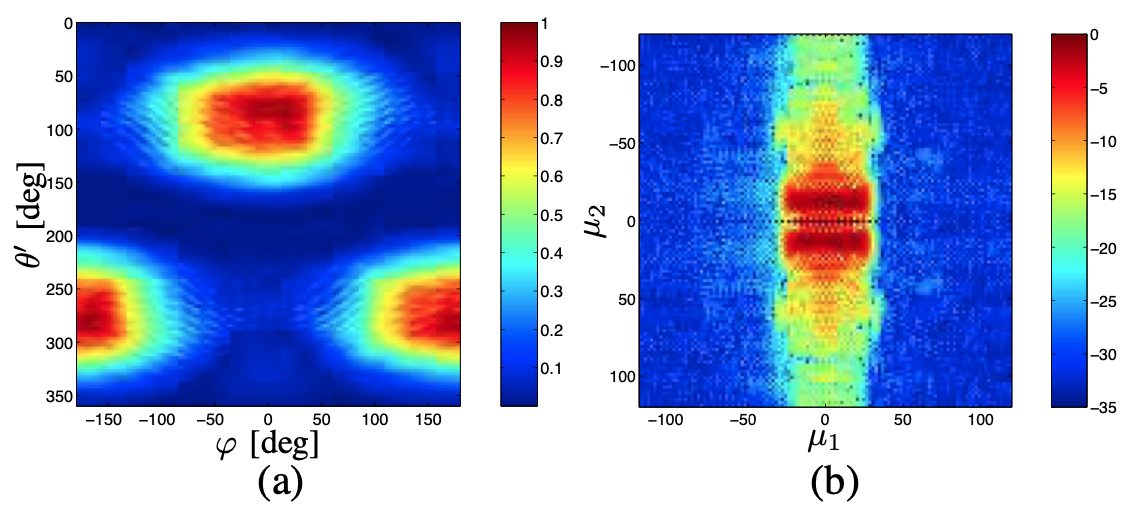
\includegraphics[width=0.75\textwidth]{img/eadf/bp_aperture.png}
    \caption{Links: Periodifizertes 2D Array $a[n_\varphi, n_\vartheta]$ der gemessenen Amplituden eines einzelnen Patch-Elements. Rechts: Der Betrag der zugeh\"origen \gls{eadf}, wobei hier $\mu_1 = k_\varphi$ und $\mu_2 = k_\vartheta$. Grafik aus~\cite{landmann2004EADF}}\label{eadf_bp_aperture}
\end{figure}

Die Bandlimitierung von $a$ l\"asst sich formulieren, indem man fordert, dass die Bedingungen
\begin{align}
    A_{\varphi}(F_\varphi, \vartheta) 
    &= \Int{-\infty}{+\infty}{
        a(\varphi, \vartheta) \exp(\jmath 2 \pi F_\varphi \varphi)
    }{\varphi} = 0 
    \fuer F_\varphi > B_\varphi \Text{und alle} \vartheta \in [0, 2 \pi] \Text{und} \\
    A_{\vartheta}(\varphi, F_\vartheta) 
    &= \Int{-\infty}{+\infty}{
        a(\varphi, \vartheta) \exp(\jmath 2 \pi F_\vartheta \vartheta)
    }{\varphi} = 0 
    \fuer F_\vartheta > B_\vartheta \Text{und alle} \varphi \in [0, 2 \pi]
\end{align}
erf\"ullt sein m\"ussen. Nun lassen sich alle obigen Argumente ``schnittweise'' auf eine abgetastete Version von $a$ in der Form $a[n_\varphi, n_\vartheta]$ anwenden. Das hei{\ss}t, wir landen schlussendlich bei einer Interpolations-Formel
\begin{equation}\label{2d_dft_interpolation}
    a(\varphi, \vartheta) = \Sum{k_\varphi=-\frac{B_\varphi}{F_\varphi}}{+\frac{B_\varphi}{F_\varphi}}{
        \Sum{k_\vartheta=-\frac{B_\vartheta}{F_\vartheta}}{+\frac{B_\vartheta}{F_\vartheta}}{
            A[k_\varphi, k_\vartheta] 
            \cdot \exp(\jmath 2 \pi k_\varphi \varphi F_\varphi)
            \cdot \exp(\jmath 2 \pi k_\vartheta \vartheta F_\vartheta)
        }
    },
\end{equation}
welche eine absolut analoge (nicht als Gegenteil zu digitale) $2D$-Version zu \eqref{dft_interpolation} darstellt. Auch in diesem Fall, k\"onnen wir das $2D$-Array $A[k_\varphi, k_\vartheta]$ durch eine $2D$-\gls{dft}, bzw. der \gls{fft}~\cite{FFTW05}, von den uniformen Samples $a[n_\varphi, n_\vartheta]$ der Funktion $a$ effizient vorberechnen.

Um einen m\"oglichst effizienten Algorithmus f\"ur die Auswertung der Interpolante zu erhalten, sollte man \eqref{2d_dft_interpolation} geeignet umschreiben. Moderne Rechenarchitekturen und Scientific-Computing-Libraries sind auf schnelle Matrix-Vektor-Produkte optimiert. Nehmen wir an, wir wollen \eqref{2d_dft_interpolation} f\"ur mehrere Winkelpaare $(\varphi_1, \vartheta_1), \dots, (\varphi_L, \vartheta_L)$ auswerten. Dann berechnen wir zun\"achst zwei $2D$ Arrays
\begin{align}
    D_\varphi &= [\exp(\jmath 2 \pi k_\varphi \varphi F_\varphi)]_{\ell = 1, k_\varphi=-\frac{B_\varphi}{F_\varphi}} \in \C^{L \times 2 \frac{B_\varphi}{F_\varphi} + 1} \Text{und}\\
    D_\vartheta &= [\exp(\jmath 2 \pi k_\vartheta \vartheta F_\vartheta)]_{\ell = 1, k_\vartheta=-\frac{B_\vartheta}{F_\vartheta}} \in \C^{L \times 2 \frac{B_\vartheta}{F_\vartheta} + 1}, 
\end{align}
was uns erlaubt \eqref{2d_dft_interpolation} in das folgende Vektor-Matrix-Vektor-Produkt
\begin{equation}\label{fast_2d_dft}
    a(\varphi_\ell, \vartheta_\ell) = 
        D_\varphi[\ell, :] \cdot A[:,:] \cdot D_\vartheta[\ell, :]^\trans
\end{equation}
umzuschreiben. Damit besteht der Interpolations-Algorithmus zun\"achst aus der Vorberechnung des Arrays $A$, sowie bei Ausf\"uhrung dann aus der Berechnung von $D_\varphi$ und $D_\vartheta$, sowie der Auswertung von \eqref{fast_2d_dft}.

Man sieht hier der sch\"on, dass die Laufzeitkomplexit\"at von \eqref{fast_2d_dft} ma{\ss}geblich von der r\"aumlichen Bandbegrenzung der Antennen-Richtcharakteristik beeinflusst wird. Je h\"oher die Bandbreite, desto h\"oher ist nicht nur der Aufwand bei der Messung, sondern auch bei der Interpolation. Eine alternative Form der Interpolation, welche diese eventuell nachteilige Eigenschaft nicht hat, ist in \Cref{b-splines} dargestellt.

%
%
%
\clearpage
\microtypesetup{protrusion=false}
\addcontentsline{toc}{section}{Abk"urzungsverzeichnis}
\printglossary[type=\acronymtype]
\microtypesetup{protrusion=true}
%
%
%
\clearpage
\microtypesetup{protrusion=false}
\addcontentsline{toc}{section}{Literaturverzeichnis}
\printbibliography
\microtypesetup{protrusion=true}
\end{document}